\documentclass[a4paper,11pt]{article}
\usepackage[margin=2cm]{geometry}

\usepackage[titletoc,toc,title,page]{appendix}
\usepackage[nodayofweek]{datetime}
\usepackage{cite}
\usepackage{graphicx}
\longdate

\usepackage{paralist}
\usepackage{mathcomp}
\usepackage{bm}
\usepackage{amsmath,amssymb,amsthm,enumitem}
\usepackage{graphicx}
\usepackage{caption}
\usepackage{subcaption}
\usepackage{titlesec}
\usepackage{array,multirow}
\newcolumntype{C}[1]{>{\centering\let\newline\\\arraybackslash\hspace{0pt}}m{#1}}

\setcounter{secnumdepth}{4}

\usepackage{hyperref}
\usepackage{fancyhdr}
\usepackage{minted}
\pagestyle{fancyplain}
\fancyhf{}
\lhead{\fancyplain{}{MSc Individual Project Report}}
\rhead{\fancyplain{}{\today}}
\cfoot{\fancyplain{}{\thepage}}

\newcommand{\reporttitle}{Information Theory and Metastability in Neural Populations}
\newcommand{\reportauthor}{Juan Carlos Farah}
\newcommand{\supervisor}{Professor Murray Shanahan\\Pedro Mediano}
\newcommand{\degreetype}{MSc Computing}

\begin{document}

% load title page
\newcommand{\HRule}{\rule{\linewidth}{0.5mm}}

%----------------------------------------------------------------------------------------
%	LOGO SECTION
%----------------------------------------------------------------------------------------

\includegraphics[width = 4cm]{./figures/imperial}\\[0.5cm]

\begin{center}

%----------------------------------------------------------------------------------------
%	HEADING SECTIONS
%----------------------------------------------------------------------------------------

\textsc{\Large Imperial College London}\\[0.5cm]
\textsc{\large Department of Computing}\\[0.5cm]

%----------------------------------------------------------------------------------------
%	TITLE SECTION
%----------------------------------------------------------------------------------------

\HRule \\[0.4cm]
{ \huge \bfseries \reporttitle}\\
\HRule \\[1.5cm]

%----------------------------------------------------------------------------------------
%	AUTHOR SECTION
%----------------------------------------------------------------------------------------

\begin{minipage}{0.4\textwidth}
\begin{flushleft} \large
\emph{Author:}\\
\reportauthor
\end{flushleft}
\end{minipage}
~
\begin{minipage}{0.4\textwidth}
\begin{flushright} \large
\emph{Supervisors:} \\
\supervisor
\end{flushright}
\end{minipage}\\[4cm]


%----------------------------------------------------------------------------------------
%	FOOTER & DATE SECTION
%----------------------------------------------------------------------------------------
\vfill % Fill the rest of the page with whitespace
Submitted in partial fulfillment of the requirements for the MSc degree in
\degreetype~of Imperial College London\\[0.5cm]

\makeatletter
\@date
\makeatother

\end{center}

\clearpage

\tableofcontents

\clearpage

\section{Introduction}

In the brain, metastability is defined as the ``simultaneous realisation of two competing tendencies: the tendency of the individual components to couple together and the tendency for the components to express their independent behaviour'' \cite{Kelso2012}. The Theory of Coordination Dynamics postulates that metastability is a key aspect of neurodynamics and it has been suggested that it plays an important role in several cognitive functions and consciousness \cite{Seth2009}. 

Over the past ten years, the Integrated Information Theory of Consciousness (IIT) has arisen as a possible framework to explain the nature and properties of consciousness. The IIT claims that consciousness can be measured by a system's ability to integrate information, that is, to what extent information is generated by a system as a whole and not by the sum of its parts \cite{Tononi2008a}.

By modelling synchronisation using spiking neural networks and large-scale approximations such as oscillators following the Kuramoto model, this project aims to investigate the properties of metastability and consciousness from an information-theoretic point of view. Specifically, we will conduct a series of simulations to study the correspondence between several properties of these networks, some of which are highlighted in Section \ref{Measures}, with a particular focus on how they relate to integrated information. Our goal is to shed light on the dynamics and properties of information transmission and processing between populations of neurons as they oscillate in and out of transient coupled states.

\section{Background}

This project will focus on a number of concepts from the fields of Information Theory and Computational Neurodynamics. In order to motivate their inclusion in this study and introduce the structures and measures used, this section provides a general explanation of these terms.

\subsection{Kuramoto Model}
\label{KuramotoModel}

The Kuramoto model, proposed by Yoshiki Kuramoto, is a mathematical model for a system of coupled phase oscillators. It has widespread use in neuroscience as a framework for the study of synchronisation in dynamical systems as observed in nature \cite{Cumin2007}. The dynamics of this model are an extension of work by Winfree, which Kuramoto generalised to the form shown in equation \ref{eq:kuramoto} \cite{Strogatz2000}, where $N$ is the number of coupled phase oscillators $\theta_{i}(t)$ with natural frequencies $\omega_{i}$ distributed over $g(\omega)$.

\begin{equation} \label{eq:kuramoto}
\dot{\theta_i} = \omega_i + \sum_{j=1}^{N} K_{ij} \sin(\theta_j - \theta_i), i = 1, ..., N
\end{equation}


\subsection{Networks of Spiking Neurons}

As further explained in Section \ref{MSUSNN}, we will model populations of spiking neurons in order to analyse more fine-grained properties of the network, such as its spectral complexity. The models that we will used will be based on work by Buehlmann and Deco \cite{Buehlmann2010} as well as by Bhowmik and Shanahan \cite{Bhowmik2013}. For the neurons in our networks we will use the widely used Hodgkin-Huxley model \cite{Hodgkin1952}. ``Hodgkin and Huxley found three different types of ion current: sodium (Na+), potassium (K+), and a leak current that consists mainly of chloride (Cl2) ions. Different voltage-dependent ion channels control the flow of ions through the cell membrane.'' \cite{Bhowmik2013}

For the dynamics of the neurons in our network we will follow the Quadratic Integrate-and-Fire (QIF) model. The change in membrane potential over time of QIF neurons is given by the following equations, where $V$ is the membrane potential, $V_r$ is the resting potential, $V_t$ is the firing threshold, $C$ is the membrane capacitance, $\tau$ is the membrane time  constant, $I$ is the current and $R$ the resistance.

\begin{equation} \label{eq:qif}
\frac{dV}{dt} = \frac{1}{\tau}(V - V_ r)(V-V_t) +  \frac{I}{C}
\end{equation}

\begin{equation} \label{eq:tau}
\tau = RC
\end{equation}

Intially, as in \cite{Bhowmik2013} we will set $\frac{1}{\tau} = 2$ and assume a membrane potential between $V_r = 265$ mV and $V_t = 245$ mV. However, depending on the results of our simulations, we might be inclined to fine-tune these values to better fit our requirements.

\subsection{Metastability}

It has been observed that ``periodic phenomena involving the synchronisation of multiple variables are prevalent both in nature and the human environment'' \cite{Shanahan2010} and these have been successfully modelled using systems of coupled oscillators such as those described in Section \ref{KuramotoModel}. Several studies have focused on investigating how these systems exhibit stable states of synchronisation \cite{Acebron2005}. However, increased long-distance synchronisation has also been linked to pathological behaviours such as epileptic seizures \cite{Arthuis2009}, which motivates the study of recurring, shorter bursts of synchronisation between oscillating structures that occur alongside periods of desynchronisation. This behaviour is defined as metastability. ``A system of oscillators exhibits metastability if some or all of its members linger in the vicinity of a synchronised state without falling into such a state permanently.'' \cite{Shanahan2010}


``Metastability is quantified by the variance of synchrony within an individual oscillator cluster over time, averaged for all clusters in the system, and so characterizes the tendency of a system to continuously migrate between a variety of synchronous states.'' \cite{Bhowmik2013}

% ==============
% CHIMERA STATES
% ==============
\subsection{Chimera States}
\label{sec:bg:chimera}

As explained in \cite{Shanahan2010}, competition is a feature of many complex systems. In the brain, one of the ways in which competition manifests itself is in the presence of chimera states. Chimera states refer to the phenomena where a coalition of populations of neurons (or oscillators) are synchronised while other coalitions are desynchronised. This can be seen from milliseconds 310 to 330 in Figure \ref{Shanahan2010_Chimera}. We observe that the black, red, blue, green and purple communities are synchronised while the gray, turquoise and mustard communities are desynchronised.

\begin{figure}[H]
\centering
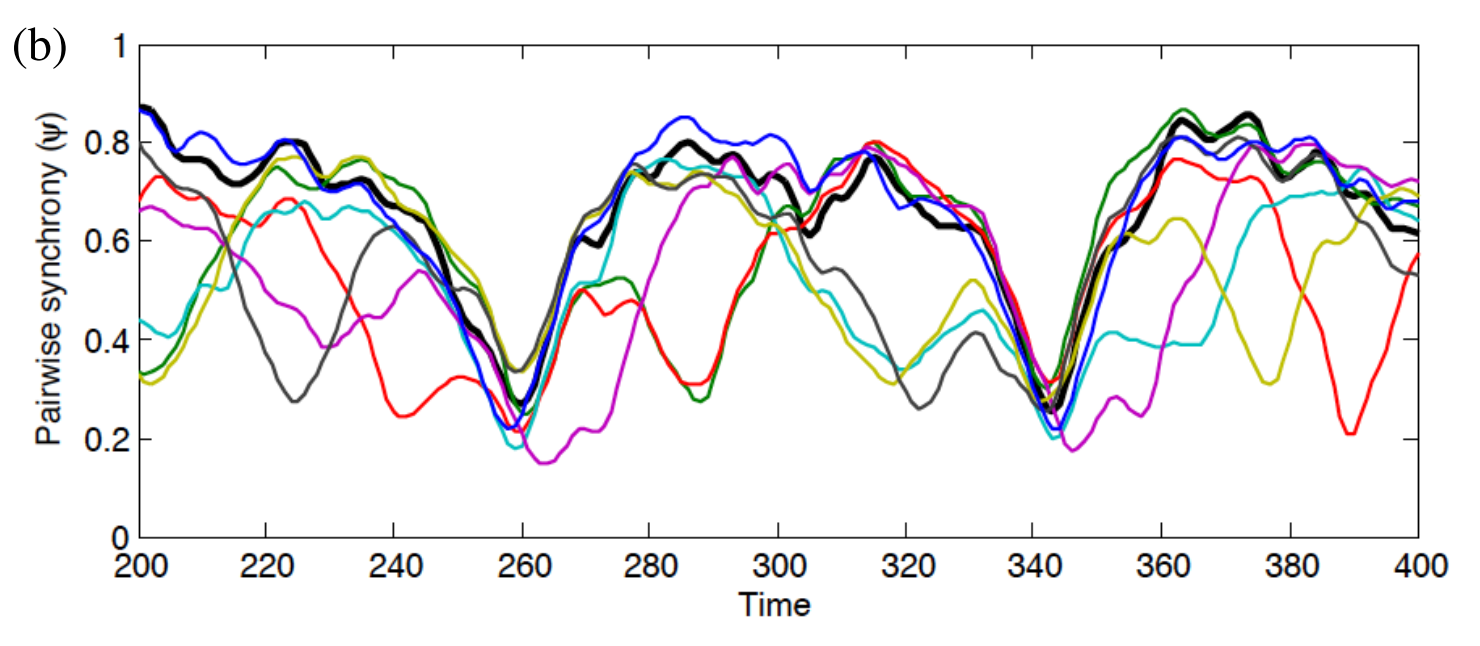
\includegraphics[scale = 0.5]{Shanahan2010_Chimera}
\caption{
	``Inter-community synchrony: Pairwise synchrony is plotted between one selected community (shown in black) and each of the eight communities (including itself). From time 310 to 330 the selected community is synchronised with several others, forming a temporary coalition.'' \cite{Shanahan2010}
	\label{Shanahan2010_Chimera}
}
\end{figure}

\subsection{Integrated Information Theory of Consciousness}
In 2004, Tononi presented his Integrated Information Theory, postulating that consciousness could be defined as the capacity of a system to integrate information \cite{Tononi2004}. He claimed that there were two major problems posed by consciousness. The first concerns the issue of how to determine if and to what extent a system experiences consciousness. That is, what can be measured to determine the consciousness of a given system. The second is related to the type of consciousness that a system may have. That is, addressing the fact that different kinds of conscious experiences are associated to different parts of the brain and how damage to one of these areas can affect one type of sensory experience, but leave others unaffected (e.g. certain lesions only affect one's capability to perceive colours).

We will focus on the former of these concerns. Tononi proposed that a good measure for consciousness would be $\Phi$, which computes a system's ability to generate information as a whole, rather than as a sum of its parts. We further explain integrated information in Section \ref{II}.

% ========
% MEASURES
% ========
\subsection{Measures}
\label{Measures}
In this section we provide an overview of the different information-theoretic measure that we will use to analyse the neural populations and networks of oscillators used in this study.

% -------
% Entropy
% -------
\subsubsection{Entropy}
\label{sec:bg:entropy}

Entropy $H$ is a measure of uncertainty and for a discrete random variable $X$ that takes values in the space $\Omega_X$, can be calculated as shown in Equation \ref{eq:entropy}.

\begin{equation} \label{eq:entropy}
H(X) = - \sum_{x \in \Omega_X}P_X(x) \log_2 P_X(x)\\[2.5mm]
\end{equation}

% -------------------
% Conditional Entropy
% -------------------
\subsubsection{Conditional Entropy}
\label{sec:bg:cond-entropy}

The expected conditional entropy of $X$ given $Y$, where $Y$ is a discrete random variable that takes values in the space $\Omega_Y$, is denoted $H(X|Y)$ and calculated as shown in Equation \ref{eq:cond-entropy}.

\begin{equation}
\label{eq:cond-entropy}
H(X|Y) = \sum_{y \in \Omega_Y}H(X|Y=y)P_Y(y)
\end{equation}

% ------------------
% Mutual Information
% ------------------
\subsubsection{Mutual Information}
\label{sec:bg:mi}

The mutual information $I(X,Y)$ between $X$ and $Y$ is the reduction in entropy of $X$ given that we know $Y$. It is calculated as shown in Equation \ref{eq:mi}.

\begin{equation}
\label{eq:mi}
I(X,Y) = H(X) - H(X|Y)
\end{equation}

% ---------------------------
% Kullback-Leibler Divergence
% ---------------------------
\subsubsection{Kullback-Leibler Divergence}
\label{sec:bg:kld}

The Kullback-Leibler divergence $D_{KL}(P || Q)$ quantifies the difference between two probability distributions $P$ and $Q$. It is a non-symmetric, non-negative measure that computes the information lost when Q is used to approximate P \cite{Burnham2002}. It is calculated as shown in equation \ref{eq:kld}.

\begin{equation}
\label{eq:kld}
D_{KL}(P || Q) = \sum_{i} P(i) ln \frac{P(i)}{Q(i)}
\end{equation}

% ---------
% Synchrony
% ---------
\subsubsection{Synchrony}
\label{sec:bg:sync}

In order to quantify how synchronised the oscillators within a given community are at a given time step $t$, you can use Equation \ref{eq:sync} to calculate $\psi_c(t)$\cite{Shanahan2010}. 

\begin{equation} \label{eq:sync}
\psi_c(t) = |\langle e^{i\theta_k(t)}\rangle_{k \in c}|
\end{equation}

Here, $e^{i\theta_k(t)}$, which raises $e$ to the power of $i = \sqrt{-1}$ and multiplies that by $\theta_k(t)$, the phase of oscillator $k$ at time step $t$, is averaged over all oscillators in community $c$. This produces a value that ranges from zero when all the oscillators are completely desynchronised to one, when they are all in synchrony \cite{Shanahan2010}.

% ----------------
% Global Synchrony
% ----------------
\subsubsection{Global Synchrony}
\label{sec:bg:global-sync}

Once you have calculated the synchrony of a community of oscillators $c$ for each time step $t$, you can average this for all of the time steps in a given simulation $T$ to obtain an aggregate measure of synchrony for that community ($\widehat{\psi}$), as shown in Equation \ref{eq:comm-sync}.  To obtain the global synchrony ($\Psi$), as given by Equation \ref{eq:global-sync}, you simply average $\widehat{\psi}$ over all the communities $c$ in a given population $C$ \cite{Shanahan2010}.

\begin{equation} \label{eq:comm-sync}
\widehat{\psi}_c = \frac{1}{|T|} \sum_{t \in T} \psi_c(t)
\end{equation}

\begin{equation} \label{eq:global-sync}
\Psi = \frac{1}{|C|} \sum_{c \in C} \widehat{\psi}_c
\end{equation}
 
% -------------------
% Metastability Index
% -------------------
\subsubsection{Metastability Index ($\lambda$)}
\label{sec:bg:lambda}

In \cite{Shanahan2010}, Shanahan proposes an index for metastability that builds on the synchrony measure described in Section \ref{sec:bg:sync}. We take $\psi_t$ for a given community $c$ over all time step $t \in T$, where $T$ is the total number of time steps in the simulation, and then measure the variance over $T$, as denoted in Equation \ref{eq:sigma-met}. This measure can then be averaged over all communities $c$ in the system $C$ to produce an index of how metastable the population is overall. We call this measure $\lambda$ following the nomenclature established in \cite{Shanahan2010} as presented in Equation \ref{eq:lambda}.

\begin{equation} \label{eq:sigma-met}
\sigma_{\psi}(c) = \frac{1}{T - 1} \sum_{t \leq T }(\psi_{c}(t) - \langle \psi_{c}\rangle_T)^2
\end{equation}

\begin{equation} \label{eq:lambda}
\lambda = \langle \sigma_{\psi} \rangle_C
\end{equation}

% -------------
% Chimera Index
% -------------
\subsubsection{Chimera Index ($\chi$)}
\label{sec:bg:chi}

In order to calculate how chimera-like a system is at a given time step, we follow \cite{Shanahan2010, Bhowmik2013}, fix time and calculate the variance across communities. This indicates ``the level of spontaneous partitioning into synchronized and desynchronized subsets'' \cite{Bhowmik2013} and can be averaged as in \cite{Shanahan2010} to calculate $\chi$ shown below, where $C$ is the set of $M$ number of communities and $\psi_c(t)$ is the synchrony of community $c$ at time $t$ as described in Section \ref{sec:bg:sync}.

\begin{equation} \label{eq:var-sync}
\sigma_{chi}(t) = \frac{1}{M - 1}\sum_{c \in C}(\psi_c(t) - \langle \psi(t) \rangle_C)^2
\end{equation}

\begin{equation} \label{eq:chi}
\chi = \langle \sigma_{chi} \rangle_T
\end{equation}


% -----------------
% Coalition Entropy
% -----------------
\subsubsection{Coalition Entropy} \label{sec:bg:hc}

``Coalition entropy measures the variety of metastable states entered by a system of oscillators and is calculated from the number of distinct states the system can generate and the probability of each state occurring.'' \cite{Bhowmik2013} We can calculate the coalition entropy $H_C$ for a system by computing ``how `mixed up' is the set of coalitions a system produces over a period of time'' \cite{Shanahan2010}. This is given by the equation below where ``$S$ is the set of distinct coalitions the system can generate and $p(s)$ is the probability of coalition $s$ arising in any given time point'' \cite{Shanahan2010}.

\begin{equation} \label{eq:hc}
H_C = - \frac{1}{\log_2 |S|}\sum_{s \in S}p(s) \log_2 (p(s))
\end{equation}

% ----------------
% Transfer Entropy
% ----------------
\subsubsection{Transfer Entropy}
Transfer entropy ``is an information theoretical measure that quantifies the statistical coherence between systems. It has the advantage that it does not only measure the coherence between two signals, but is able to distinguish between driving and responding elements and therefore between shared and transported information. This is called the directionality of the information flow.'' \cite{Buehlmann2010} Transfer entropy from process $J$ to process $I$ can be calculated using the equation below, where $l = k$ or $l = 1$ \cite{Schreiber2000}.

\begin{equation} \label{eq:te}
T_{J \rightarrow I} = \sum p(i_{n+1}, i_{n}^{(k)}, j_{n}^{(l)}) \log_2 \frac{p(i_{n+1} | i_{n}^{(k)}, j_{n}^{(l)})}{p(i_{n+1} | i_{n}^{(k)})}
\end{equation}

% ---------------------
% Effective Information
% ---------------------
\subsubsection{Effective Information}
\label{EI}

The effective information, $\phi$ of a system given a bipartition $\mathcal{B} = \lbrace P^1, P^2 \rbrace$ represents how much more information is generated by the whole system than by each member of $\mathcal{B}$. Specifically, if we want to calculate the effective information given the current state $X_t$ regarding the previous state $X_{t - \tau}$, with respect to bipartition $\mathcal{B}$, we sum the mutual information generated by each of the parts in $\mathcal{B}$ and subtract that from the mutual information generated by the whole system.

\begin{equation} \label{eq:ei}
\phi [X, \tau, \mathcal{B}] = I(X_{t-\tau}, X_t) - \sum_{k=1}^{2} I(P_{t-\tau}^k, P_{t}^k)
\end{equation}

% ----------------------
% Stochastic Interaction
% ----------------------
\subsubsection{Stochastic Interaction}
\label{sec:bg:stochastic}

A slight variation of effective information known as stochastic interaction ($\tilde{\phi}$), which is also known as expected effective information \cite{Barrett2011}. It is defined as the average Kullback-Leibler divergence between the past state given the present state of system as a whole and the product of this for each subsystem given a set of partitions \cite{Ay2015}. For our purposes, as we will only be considering bipartitions, we can use the form presented by Barrett and Seth in \cite{Barrett2011}, as shown in Equation \ref{eq:stochastic}.

\begin{equation} \label{eq:stochastic}
\tilde{\phi} [X, \tau, \{M^1, M^2\}] = \sum_{k=1}^{2} H(M_{t-\tau}^k | M_{t}^k)  - H(X_{t-\tau} | X_t)
\end{equation}

% ----------------------
% Integrated Information
% ----------------------
\subsubsection{Integrated Information}
\label{II}

As noted in \cite{Barrett2011}, there are several definitions of integrated information. We will be using the empirical definition of integrated information, $\Phi_{E}$, as well as well as a slightly modified version, $\widetilde{\Phi}_{E}$ as put forth in \cite{Barrett2011}.\\

\noindent\textbf{Empirical Integrated Information ($\Phi_{E}$)}\\[2.5mm]
\noindent Empirical integrated information, $\Phi_{E}$, is a version of integrated information that is best suited for time series data such as the one we will be using in our study. It is defined as the effective information of a system with respect to its minimum information bipartition.

\begin{equation} \label{eq:ii}
\Phi [X, \tau] = \phi [X, \tau, \mathcal{B}^{MIB}(X, \tau)]
\end{equation}

\begin{equation} \label{eq:mib}
\mathcal{B}^{MIB}(X, \tau) = \arg_{\mathcal{B}} \min \Big\lbrace \frac{\phi [X, \tau, \mathcal{B}]}{K(\mathcal{B})} \Big\rbrace
\end{equation}

\begin{equation} \label{eq:norm}
K(\mathcal{B} = \lbrace P^1, P^2 \rbrace) = \min[H(P^1), H(P^2)]\\[2.5mm]
\end{equation}

\noindent\textbf{Empirical Integrated Information Tilde ($\widetilde{\Phi}_{E}$)}\\[2.5mm]
\noindent Empirical integrated information tilde, $\widetilde{\Phi}_{E}$, is a variation of $\Phi_{E}$ that uses stochastic interaction instead of effective information in order to determine the minimum information bipartition. Overall, $\widetilde{\Phi}_{E}$ behaves very similarly to $\Phi_{E}$, although it provides certain useful properties such as the fact that it will never give a negative value.

\begin{equation} \label{eq:ii-tilde}
\widetilde{\Phi} [X, \tau] = \tilde{\phi} [X, \tau, \widetilde{\mathcal{B}}^{MIB}(X, \tau)]
\end{equation}

\begin{equation} \label{eq:mib-tilde}
\widetilde{\mathcal{B}}^{MIB}(X, \tau) = \arg_{\widetilde{\mathcal{B}}} \min \Big\lbrace \frac{\tilde{\phi} [X, \tau, \widetilde{\mathcal{B}}]}{\widetilde{K}(\widetilde{\mathcal{B}})} \Big\rbrace
\end{equation}

\begin{equation} \label{eq:norm-tilde}
\widetilde{K}(\widetilde{\mathcal{B}} = \lbrace P^1, P^2 \rbrace) = \min[H(P^1), H(P^2)]
\end{equation}


\subsection{Related Experimental Work}
\begin{enumerate}
\item{We know that information measures are related to consciousness.}
\item{We know that metastability is related to consciousness}
\item{What we want to see is if information measures are related to metastability.}
\end{enumerate}

\begin{enumerate}
\item{Return to consciousness.}
\item{Information Sharing in the Brain Indexes Conscious in Noncommunicative Patients}
\item{Symbolic Analysis - Allow this to work.}
\end{enumerate}

\subsection{Shanahan, Deco, Bhowmik}

% =======================================================================================
% IMPLEMENTATION
% =======================================================================================
\clearpage
\section{Implementation of Integrated Information ($\Phi$)}
\label{sec:impl}

In order to calculate the values of $\Phi$ for our sample populations, we implemented functions that compute Empirical Integrated Information ($\Phi_{E}$) and Empirical Integrated Information Tilde ($\widetilde{\Phi}_{E}$), as described in Section \ref{II}. We decided that it would be best that these functions be available as part of the Java Information Dynamics Toolkit (JIDT) developed by Lizier and widely used to study the dynamics of complex systems \cite{Lizier2014}. Written completely in Java, our implementation follows the syntax, semantics and structure of other features in the JIDT, which is geared towards facilitating its adoption by its current users.

\subsection{Methodology}

The structure put forth by the JIDT consists of defining a Java class that can calculate the measure in question. This class then exposes a series a methods that allow the user to bind the data that will be used for the calculation as well as perform any ancillary or preparatory operations required to compute the measure. Finally, the class will have a method to carry out the calculation and return the required output. Once an object of the calculator class is instantiated, it can be used for multiple calculations by binding new data to it and reinitialising the object's properties if needed. 

Another feature of the JIDT is that for most measures it supports, it defines a calculator both for the discrete and continuous versions of the measures, if applicable. For instance, it has a class to calculate entropy from continuous data called \texttt{EntropyCalculator} and its corresponding version for discrete data called \texttt{EntropyCalculatorDiscrete}. In some cases, it even defines a third version for mixed data, such as is the case for multivariate conditional mutual information. For our purposes, we are only interested in calculating the integrated information from discrete time series data and thus we have focused our efforts to implement a robust calculator for discrete data. Nevertheless, extending the implementation for continuous data would be useful in order to increment the breadth of the JIDT and is suggested as a possible extension to the project.

\begin{figure}[H]
\begin{center}
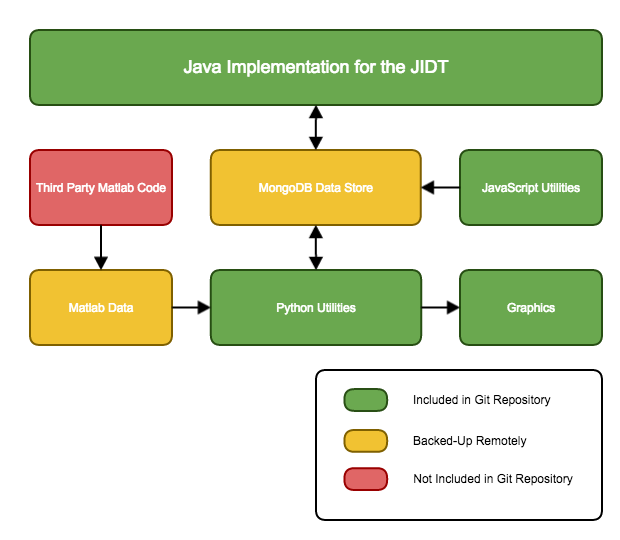
\includegraphics[scale = 0.5]{figures/architecture}
\caption{
	Architecture for the software included in this project.
	\label{fig:architecture}
}
\end{center}
\end{figure}

\subsection{Architecture}

In addition to our implementation of $\Phi$ in Java for the JIDT, our project required a suite of tools and a supporting stack to facilitate the import, export and storage of data as well as a rigorous source version control system in order to facilitate integration with the JIDT. We thus decided to develop the utilities in Python and JavaScript, and use MongoDB \cite{MongoDB} as the database layer for the data inputted to and outputted from our simulations. The Python utilities also allowed us to import the Matlab data files outputted by third party codebases adapted from \cite{Shanahan2010} and \cite{Bhowmik2013}, which we ran in our simulations. Additionally, the Python utilities were used to fetch stored data, plot and export them as graphics for our analysis. This gave us the flexibility to be able to study the data generated by our simulations without having to run them every time. We used Git as our version control system, hosting our remote repository on \href{http://github.com}{GitHub} \cite{GitHub}, which will allow us to easily integrate with the future GitHub JIDT repository. The high level architecture of our implementation is depicted in Figure \ref{fig:architecture}.

\subsection{Empirical Integrated Information}
\label{sec:impl:phi-e}

\subsubsection{Discrete Effective Information Calculator}
\label{sec:impl:ei}

In order to calculate the integrated information of a system, by definition you need to calculate its effective information. We implemented a class that computes the effective information of time-series data given a time-step $\tau$, the number of input states for each variable in the input $base$, and a bipartition $\mathcal{B}$. As shown below, you initialise the calculator for a given base and $\tau$. You then bind the input data to the calculator object using its \texttt{addObservations} method.

\begin{minted}{java}
// Initialise effective information calculator.
EffectiveInformationCalculatorDiscrete eicd;
eicd = new EffectiveInformationCalculatorDiscrete(base, tau);
eicd.addObservations(input);
\end{minted}

As explained in Section \ref{EI} the effective information of a system given a bipartition $\mathcal{B}$ for a given time step $\tau$ represents the difference between the mutual information of the whole system given the current state $X_t$ regarding a previous state $X_{t-\tau}$ and the sum of the respective mutual information for each member of $\mathcal{B}$. In order to avoid calculating the mutual information of the system for each partition that is passed to the calculator, the \texttt{EffectiveInformationCalculatorDiscrete} class has a method \texttt{computeMutualInformationForSystem}, which only needs to run once for a given data set, as it stores the result in the system property of the class.

At this point you are able to compute the effective information for a given bipartition with the method \texttt{computeForBipartition}. The latter takes a partition as an argument in the form of an integer array specifying which variables to consider as one of the partitions of the system.

\begin{minted}{java}
// Calculate mutual information for the system.
double output = eicd.computeMutualInformationForSystem();

// Calculate effective information given a partition.
int[] partition = {0, 1, 2};
double output = eicd.computeForBipartition(partition);
\end{minted}


\noindent \textbf{Input}\\

\noindent The \texttt{EffectiveInformationCalculatorDiscrete} class takes advantage of JIDT's MutualInformationCalculatorDiscrete class in order to compute the mutual information of the system and each bipartition. However, this class does not expose a method to calculate the mutual information for two-dimensional inputs. Hence we created a special Input class with two main purposes.

\begin{enumerate}
\item{To reduce the time series input to one dimension.}
\item{To pair the input value at time step $t$ with that at $t-\tau$.}
\end{enumerate}

We achieve the first by taking advantage of JIDT's \texttt{MatrixUtils}. \texttt{MatrixUtils} exposes a method called \texttt{computeCombinedValues} which effectively reduces a two-dimensional array to a one-dimensional. Because computeCombinedValues performs the reduction in a row-wise fashion and our time-series input requires a column-wise reduction, we also take advantage of \texttt{MatrixUtils}' transpose method. We also track the change in base, which will equal the original base to the power of the number of variables, as it is needed to calculate the effective information. All this functionality is exposed in \texttt{Input}'s \texttt{reduce} method.

Once the \texttt{Input} object has been reduced, you can pair the inputs using the pair method. For this we simply take the reduced array $R$ of length $n$ and the time step $\tau$, and output an $n \times 2$ matrix $P$ where the first array contains the first $n - \tau$ elements of $R$ and the second array contains the last $n - \tau$ elements. Thus each column in $P$ contains the paired values required to calculate the mutual information and each row is passed onto the \texttt{MutualInformationCalculatorDiscrete} as shown below.

\begin{minted}{java}
// Calculate MI for whole system.
Input sys = new Input(data, base);
int sysBase = sys.getReducedBase();
int[][] sysPaired = sys.pair(tau);
micd = new MutualInformationCalculatorDiscrete(sysBase, 0);
micd.initialise();
micd.addObservations(sysPaired[0], sysPaired[1]);
double system = micd.computeAverageLocalOfObservations();
\end{minted}

\subsubsection{Discrete Integrated Information Calculator}

By definition, the integrated information of a system is calculated by taking its effective information with respect to the minimum information bipartition, as explained in Section \ref{II}. Our implementation adds to the JIDT a class called \texttt{IntegratedInformationEmpiricalCalculatorDiscrete}. This calculator takes a time-series input ($data$), the number of input states for each variable in the input ($base$) and a time-step ($\tau$) to find the minimum information bipartition and in turn calculate the integrated information of the system. As with the \texttt{EffectiveInformationCalculatorDiscrete}, we follow the patterns set forth by the JIDT, so an instance of this calculator is initialised with $base$ and $tau$, and then $data$ is bound using the method \texttt{addObservations}.

\begin{minted}{java}
// Initialise integrated information calculator.
IntegratedInformationCalculatorDiscrete iicd;
iicd = new IntegratedInformationCalculatorDiscrete(base, tau);
iicd.addObservations(input);
\end{minted}

In order to find the possible partitions, the class has a method \texttt{computePossiblePartitions}, which takes advantage of JIDT's \texttt{MathUtils}' method \texttt{generateAllSets} to generate a set of all the possible partitions and store it in the calculator's partitions property.

Once the partitions have been calculated, it is possible to calculate the integrated information of the system using the method compute. This method will iterate through all of the possible bipartitions, calculate the effective information with respect to each bipartition.

\begin{minted}{java}
// Compute possible partitions and calculate integrated information.
iicd.computePossiblePartitions();
double output = iicd.compute();
\end{minted}

Note that as shown in Section \ref{II} and explained in \cite{Barrett2011}, the minimum information bipartition is calculated by finding the bipartition that minimises the effective information of the system given that bipartition divided by a normalisation factor. The normalisation factor is the minimum entropy of both parts of the bipartition. This is necessary because if a partition covers most of the system, it will provide almost as much information as the entirety of the network, which required the normalisation factor to have a bias towards more equal partitions. Our implementation incorporates this through a method \texttt{computeNormalizationFactor}, which takes advantage of JIDT's reusable \texttt{EntropyCalculatorDiscrete} to calculate the partition with the minimum entropy.

\begin{minted}{java}
public double computeNormalizationFactor(int[][] part1, int[][] part2) {

	EntropyCalculatorDiscrete ecd = new EntropyCalculatorDiscrete(base);
	ecd.initialise();
	ecd.addObservations(part1);
	double entropy1 = ecd.computeAverageLocalOfObservations();

	ecd.initialise();
	ecd.addObservations(part2);
	double entropy2 = ecd.computeAverageLocalOfObservations();

	return Math.min(entropy1, entropy2);
}
\end{minted}

The normalisation factor ($k$) is then used inside the compute method to calculate and keep track of the minimum information bipartition. If the normalisation factor is zero, it means that one of the partitions has an entropy of zero, which means that this partition will not tell us anything about the rest of the system. To avoid division by zero, we return zero in those cases, otherwise we return the normalised effective information.

\begin{minted}{java}
	double k = computeNormalizationFactor(partition);
	double ei = eicd.computeForBipartition(partition);
	double normalizedEi = (k == 0) ? 0 : ei / k;
\end{minted}

Once the iteration is complete, the effective information with respect to the $MIB$ is then returned as the system's integrated information. 

\subsection{Empirical Integrated Information Tilde}
\label{sec:impl:phi-e-tilde}

A second version of integrated information that we implemented is the empirical integrated information tilde ($\widetilde{\Phi}_{E}$). As opposed to the regular empirical integrated information, $\widetilde{\Phi}_{E}$ uses stochastic interaction instead of effective information when calculating the minimum information bipartition ($MIB$). Its advantages, as explained in Section \ref{IIT} include the fact that $\widetilde{\Phi}_{E}$ has to be positive.

\subsubsection{Discrete Stochastic Interaction Calculator}
\label{sec:impl:stochastic}

In order to calculate the integrated information tilde of a system, by definition you need to calculate its stochastic interaction. We implemented a class that computes the stochastic interaction of time-series data given a time-step $\tau$, the number of input states for each variable in the input $base$, and a bipartition $\mathcal{B}$. As shown below, you initialise the calculator for a given base and $\tau$. You then bind the input data to the calculator object using its \texttt{addObservations} method.

\begin{minted}{java}
// Initialise stochastic interaction calculator.
StochasticInteractionCalculatorDiscrete sicd;
sicd = new StochasticInteractionCalculatorDiscrete(base, tau);
sicd.addObservations(data);
\end{minted}

As noted in Section \ref{SI}, the stochastic interaction of a system given a bipartition $\mathcal{B}$ for a given time step $\tau$ represents the difference between the sum of the conditional entropy of each member of $B$ at state $X_{t-\tau}$ given state $X_t$ and the respective conditional entropy for system as a whole. We followed the same structure used for the \texttt{EffectiveInformationCalculatorDiscrete} class, so in order to avoid calculating the conditional entropy of the system for each partition that is passed to the calculator, the \texttt{StochasticInteractionCalculatorDiscrete} class has a method \texttt{computeConditionalEntropyForSystem}, which only needs to run once for a given data set, as it stores the result in the system property of the class. As with the effective information calculator, we use the Input class in order to transform the input to the required form for our computations.

\subsubsection{Discrete Conditional Entropy Calculator}

Because stochastic interaction requires conditional entropy to be calculated both for the system as the whole and for each partition, we required an implementation of conditional entropy suited for the JIDT. We followed the pattern set by the \texttt{MutualInformationCalculatorDiscrete} class to define a \texttt{ConditionalEntropyCalculatorDiscrete} class that takes a base as a parameter, exposes an \texttt{addObservations} method to bind input data and a compute method to calculate the conditional entropy. Given that conditional entropy can be defined as shown in equation \ref{eq:ce}, we take advantage of the already available \texttt{MutualInformationCalculatorDiscrete} and \texttt{EntropyCalculatorDiscrete} classes in our implementation for conditional entropy.

\begin{equation} \label{eq:ce}
H(X|Y) = H(X) - I(X; Y)
\end{equation}

\begin{minted}{java}
public double compute() {

	double mi = micd.computeAverageLocalOfObservations();
	double h = ecd.computeAverageLocalOfObservations();

	return h - mi;
}
\end{minted}

\subsubsection{Discrete Empirical Integrated Information Tilde Calculator}

The implementation of the \texttt{IntegratedInformationEmpiricalTildeCalculatorDiscrete} class is identical to that of the \texttt{IntegratedInformationEmpiricalCalculatorDiscrete} class with the exception that the former uses the \texttt{StochasticInteractionCalculatorDiscrete} class instead of the \texttt{EffectiveInformationCalculatorDiscrete} class. Its usage is the same and it exposes the same methods, which make the two great candidates for having a common interface defined. The possibility of improving our implementation by refactoring the common code between these two classes is further explained in Section \ref{sec:fw:jidt}.

\subsection{Helper Methods}
Additionally, our implementation adds various auxiliary methods to JIDT's helper classes, which can be also used by future developers of the toolkit.

\subsubsection{Coalition Entropy}
\label{sec:impl:hc}

As explained in Section \ref{sec:bg:hc}, coalition entropy ($H_c$) measures the diversity of states reached by a given network, calculated as shown in Equation \ref{eq:hc}. This measure is applied in \cite{Shanahan2010} on the populations of Kuramoto oscillators. Since the first application of our implementation of $\Phi$ was on data outputted using the model in \cite{Shanahan2010}, we wanted to ensure that the coalition entropy in our results was consistent with those of the original study. In order to confirm this, we implemented a coalition entropy calculator following the style of the JIDT. Being able to calculate coalition entropy also allowed us to investigate its relationship to integrated information. Its use is shown below.

\begin{minted}{java}
// Compute coalition entropy.
cecd = new CoalitionEntropyCalculatorDiscrete(base);
cecd.addObservations(obs);
double ce = cecd.compute();
\end{minted}

\subsubsection{Select All Rows Except}

Given that integrated information is deeply tied with the concept of partitions within a given network, our implementation required that we could easily extract information from our time series input data. Though the JIDT contained a method to select a given set of rows from a matrix, it did so only for two-dimensional double arrays. Hence we had to overload the method in order to support two-dimensional integer arrays. Additionally, we implemented a method in order to select all the rows in a matrix except a given set of them, whose indexes are specified as an array of integers. This method allows us to easily divide time series input data into bipartitions. 

\begin{minted}{java}
// Extracts all but the specified rows from the matrix
public static int[][] selectAllRowsExcept(int matrix[][], int rows[])
\end{minted}

\subsubsection{Contains}

Since we required a way of validating whether or not an integer was present in a given array we decided that it would be best to provide that functionality as a part of the JIDT. We thus implemented a lightweight method that takes an integer array and an integer, returning true if the integer is present in the array and false otherwise.

\begin{minted}{java}
// Returns true if an integer is contained in a array, false otherwise.
public static boolean contains(int[] array, int element)
\end{minted}

\subsubsection{Insert Vector Into Matrix}

We implemented a method to insert a vector into a matrix at a given column index, taking the vector input as an integer array. Although this implementation is specifically for integer vectors and matrices, it can be easily extended for other input types.

\begin{minted}{java}
public static void insertVectorIntoMatrix(int[] input, int[][] matrix, int column)
\end{minted}

This method is particularly useful for creating two-dimensional arrays that are then passed on to the methods that calculate the measures used in this project. Since our implementation stored data in a database that was then retrieved by iterating through a cursor, this helper method allowed us to fetch data and generate an input matrix without relying on other toolkits.

\begin{minted}{java}
// Obtain a cursor by passing a query to a MongoDB collection of documents (data).
MongoCursor<Document> cursor = data.find(eq("simulation_id", _id))
                                           .sort(ascending("_id"))
                                           .iterator();

// Insert array obtained from cursor as vector into matrix (obs).
int column = 0;
while (cursor.hasNext()) {
	Document d = cursor.next();
	ArrayList<Integer> array = (ArrayList) (d.get("data"));
	int[] vector = Ints.toArray(array);
	MatrixUtils.insertVectorIntoMatrix(vector, obs, column);
	column++;
}
\end{minted}

\subsubsection{Shuffle}

Our \texttt{shuffle} method implements Durstenfeld's version of the Fisher-Yates shuffle to provide a way of rearranging both the elements of a given array or the vectors in a two-dimensional matrix \cite{Durstenfeld1964}. The algorithm follows the procedure outlined below.

\begin{minted}{java}
Random rnd = new Random();
for (int i = array.length - 1; i > 0; i--) {

	// Get new index (between 0 and i + 1).
	int index = rnd.nextInt(i + 1);

	// Swap elements at given indexes.
	int a = array[index];
	array[index] = array[i];
	array[i] = a;
}
\end{minted}

Note that while the shuffle method for one-dimensional arrays does the shuffling in place, the method for two-dimensional inputs returns a new two-dimensional array of integers. Both methods have been implemented for integer arrays, but they could easily be extended to take other inputs. 

\begin{minted}{java}
// Shuffle array in place using Fisher Yates shuffle.
public static void shuffle(int[] array)

// Shuffle 2D matrix using Fisher Yates shuffle.
public static int[][] shuffle(int[][] matrix)
\end{minted}

\subsection{Data Sources and Data Store}

Given the computationally expensive nature of our modules' simulations, a persistent store had to be used to save the output and results of each run. For our data store we chose MongoDB, a documented-oriented database, as a data store as it provides a fast, scalable solution that does not require strict design decisions in advance. As we developed our product, MongoDB's dynamic schemas allowed us to modify our objects without having to spend considerable time fixing compatibility issues. Additionally, MongoDB documents follow a JavaScript Object Notation (JSON)-like structure, which mirrors the structure of our Python objects \cite{MongoDB}.

Additionally, the output from the populations of oscillators and spiking neurons (???), which we used as input to our integrated information calculator, were saved as Matlab files and stored directly on the filesystem. Using the Oct2Py Python Package \cite{Silvester}, which provides a Python interface to GNU Octave, an open source alternative to Matlab \cite{Eaton}, we were able to manipulate these and insert them as documents in our MongoDB instance.

\subsection{Utilities}
\label{sec:utils}
This project required a number of auxiliary tools to setup, run and analyse the data generated by the simulations using our implementation of $\Phi$. First we created utility scripts in Python that could import data into our MongoDB database. For instance, in order to input data from a Matlab or Octave file containing data outputted by a Kuramoto oscillator simulation, you simply instantiate an \texttt{OscillatorDataImporter} object, connect to the appropriate database and load the folder containing the files. Our implementation will by default import the data using multiple threads to provide different parameters for import. In the Kuramoto oscillator case, we define by default that there are five possible thresholds that define if two oscillators are synchronised or not. Hence the five import processes are run in parallel. Since MongoDB allows concurrent inserts into the same collection, this speeds up the import process significantly.

\begin{minted}{python}
data_folder = "path/to/folder"
db = "database_name"

odi = OscillatorDataImporter()
odi.connect(db)
odi.load(data_folder)
\end{minted}

After running a simulation, data is stored in MongoDB and can be retrieved for analysis and visualisation. For this purpose we defined a \texttt{DataPlotter} Python class. A \texttt{DataPlotter} object gets initialised with a database name, to which it connects. It then exposes a \text{plot} method, which can optionally take various arguments, such as a query defining what data to retrieve from the database, as well as a boolean, a file system path and a file extension to indicate if the graphics should be saved, where and in what format. By default, the graphics are not saved and all the simulations in the database are considered when plotting.

\begin{minted}{python}
query = {
	'duration': 5000,
	'num_oscillators': 8        
}

dp = DataPlotter(database="infotheoretic")
dp.plot(save=True,
        path="/path/to/my/plots",
        ext="svg",
        query=query)
\end{minted}


We also implemented a data generator in order to test our implementation using synthetic data as well as a JavaScript file that provides helper functions for MongoDB to manage the creation of indexes, rearranging of simulation data and sanity checks.

\subsection{Version Control}
Using Git as a source version control system allows us to carefully track the evolution of our codebase. Currently, the JIDT is available through a repository on \href{https://code.google.com/}{Google Code}, which does not provide the functionality required for several contributors to seamlessly work actively on an open source project. Our extension for the JIDT is hosted on GitHub, which provides an intuitive web interface allow other users to clone and fork the repository for their own deployments. Additionally they can submit pull requests to contribute to the development of the JIDT.

% =======================================================================================
% APPLICATION ON POPULATIONS OF OSCILLATORS
% =======================================================================================
\clearpage
\section{Application on Populations of Oscillators}
\label{MSUKO}

Based on work by Shanahan \cite{Shanahan2010}, we used Kuramoto oscillators to create a series of systems of communities that modelled populations of neurons exhibiting metastability and chimera states. By running simulations on these networks, we were able to create discrete time series output that indicated which communities were synchronised at any give time step. These time series were inputted into our implementations of integrated information ($\Phi$) and used to compute various measures described in \ref{sec:app:osc:measures}. We were then able to analyse how these measures interacted with $\Phi$.

% ===========
% METHODOLOGY
% ===========
\subsection{Methodology}
\label{sec:osc:methods}
Our aim was to extend the work presented in \cite{Shanahan2010} and apply them to the measures proposed by Seth and Barrett in \cite{Barrett2011}, which we implemented as examined in detail in Section \ref{sec:impl}. In order to draw strong parallels between data extracted and analysed from our simulations and findings exposed in \cite{Shanahan2010}, we replicated, where possible, the methodology, methods and calculations used by Shanahan, as explained in this section. Nevertheless, we structured our simulations and trials in a way that best fit our main purpose of analysing the behaviour of integrated information with regards to other information-theoretic measures.

% ---------
% The Model
% ---------
\subsubsection{The Model}
\label{sec:osc:mod}

In Shanahan \cite{Shanahan2010}, the model consists of eight communities of 32 Kuramoto oscillators each fully connected within their own communities and randomly connected to 32 other oscillators in the population. The phase of each oscillator is determined by equation \ref{eq:shanahan:kuramoto}, which follows from the generalised Kuramoto model shown in Equation \ref{eq:kuramoto}. 

\begin{equation} \label{eq:shanahan:kuramoto}
\frac{d\theta_i}{dt} = \omega + \frac{1}{N + 1} \sum_{j=1}^{N} K_{ij} \sin(\theta_j - \theta_i - \alpha)
\end{equation}

We preserved the parameters as used by Shanahan in \cite{Shanahan2010}, where $\omega = 1$, $N = 63$, $A = u - v$ where $u + v = 1$ and $A = 0.2$. $K_{ij}$ is then defined depending on the connection between oscillators $i$ and $j$. $K_{ij} = u$ for intra-community connections and $K_{ij} = v$ for inter-community connections and $K_{ij} = 0$ when there is no connection present. Finally, $\beta = \frac{\pi}{2} - \alpha$, which determines the phase lag.

% ---------------
% The Simulations
% ---------------
\subsubsection{The Simulations}
\label{sec:osc:sims}

In order to generate the data required to apply our implementation of $\Phi$ to the populations of Kuramoto oscillators described in Section \ref{sec:osc:mod} we carried out our own simulations using the Matlab code from \cite{Shanahan2010} as a base. Each of our 7500 trials ran for 25 seconds with a value of $\beta$ assigned randomly from $0$ to $2\pi$. Every 5ms, the internal synchrony, as defined in Equation \ref{eq:sync}, was calculated and inserted into an $8 \times 8$ matrix representing the level of synchrony between all of the communities. Thus the output for every trial was a series of 5000 matrices, each of the form shown in Table \ref{tab:mat}.


% Synchrony Matrix
% ----------------
\begin{table}[ht]
\centering

\begin{tabular}{c l | c c c c c c c c}

& & \multicolumn{8}{c}{Community \#} \\ [2mm]
& & 1 & 2 & 3 & 4 & 5 & 6 & 7 & 8 \\
\hline
\parbox[t]{2mm}{\multirow{8}{*}{\rotatebox[origin=c]{90}{Community \#}}}
& 1 & \textbf{0.29} & 0.41 & 0.16 & 0.44 & 0.13 & 0.41 & 0.51 & 0.43 \\
& 2 & 0.41 & \textbf{0.56} & 0.23 & 0.60 & 0.29 & 0.57 & 0.67 & 0.59 \\
& 3 & 0.16 & 0.23 & \textbf{0.20} & 0.30 & 0.14 & 0.23 & 0.34 & 0.26 \\
& 4 & 0.44 & 0.60 & 0.30 & \textbf{0.77} & 0.51 & 0.70 & 0.80 & 0.72 \\
& 5 & 0.13 & 0.29 & 0.14 & 0.51 & \textbf{0.35} & 0.41 & 0.51 & 0.43 \\
& 6 & 0.41 & 0.57 & 0.23 & 0.70 & 0.41 & \textbf{0.64} & 0.74 & 0.66 \\
& 7 & 0.51 & 0.67 & 0.34 & 0.80 & 0.51 & 0.74 & \textbf{0.84} & 0.76 \\
& 8 & 0.43 & 0.59 & 0.26 & 0.72 & 0.43 & 0.66 & 0.76 & \textbf{0.68} \\
\end{tabular}
\caption{Each trial outputted $5000$ $8 \times 8$ matrices displaying the synchrony measure between each of the communities. The diagonal represents the internal synchrony of each community of oscillators. \label{tab:mat}}
\end{table}

As highlighted in Table \ref{tab:mat}, we focused on the diagonal in each output matrix, which represents the internal synchronisation of each oscillator community. This implies that we are considering that if a community is internally synchronised, then it is also externally synchronised.

Once extracted, this diagonal was then discretised by applying a synchronisation threshold representing whether or not the community is considered to be synchronised or not. Though in \cite{Shanahan2010} the only synchronisation threshold used is $0.8$, when analysing our results, we applied thresholds $0.5$, $0.6$, $0.7$, $0.8$, and $0.9$ to each simulation in order to obtain a better view of the effect of varying synchronisation threshold.

As a result, for each time step we obtained an array of booleans, where $1$ represents that a community of oscillators is synchronised and $0$ that it is not. As an example, Table \ref{tab:arr} depicts the application of this procedure to the data shown in Table \ref{tab:mat} using a threshold of $0.6$.

\begin{table}[ht]
\centering
\begin{tabular}{l | c c c c c c c c}
& \multicolumn{8}{c}{Community \#} \\ [2mm]
& 1 & 2 & 3 & 4 & 5 & 6 & 7 & 8 \\
\hline
Continuous & 0.29 & 0.56 & 0.20 & 0.77 & 0.35 & 0.64 & 0.84 & 0.68 \\
Discrete & 0 & 0 & 0 & 1 & 0 & 1 & 1 & 1 \\
\end{tabular}
\caption{For each time step in a simulation, the extracted diagonal array containing continuous data was converted to discrete data by applying a threshold, in this case $0.6$. \label{tab:arr}}
\end{table}
 
Each of the extracted arrays was then transposed and inserted into an $8 \times 5000$ matrix, with each row representing a community of oscillators and each column a time step. A sample output matrix is show in Table \ref{tab:timeseries}. This provides the final output of each trial as a time series that can be inputted into our implementation of $\Phi$.

\begin{table}[ht]
\centering
\begin{tabular}{c l | C{8mm} C{8mm} C{8mm} C{8mm} C{8mm} C{8mm} C{8mm} C{8mm} C{8mm}}

& & \multicolumn{9}{c}{Time Step} \\ [2mm]
& & 1 & 2 & 3 & 4 & . . . & 4997 & 4998 & 4999 & 5000 \\
\hline
\parbox[t]{2mm}{\multirow{8}{*}{\rotatebox[origin=c]{90}{Community \#}}}
& 1 & 0 & 0 & 0 & 0 & . . . & 0 & 0 & 0 & 0 \\
& 2 & 0 & 0 & 0 & 0 & . . . & 1 & 0 & 0 & 1 \\
& 3 & 0 & 0 & 0 & 1 & . . . & 1 & 0 & 0 & 1 \\
& 4 & 0 & 0 & 1 & 1 & . . . & 0 & 0 & 0 & 0 \\
& 5 & 0 & 0 & 0 & 0 & . . . & 0 & 1 & 1 & 1 \\
& 6 & 0 & 1 & 1 & 1 & . . . & 0 & 0 & 1 & 1 \\
& 7 & 0 & 1 & 1 & 0 & . . . & 1 & 1 & 1 & 1 \\
& 8 & 0 & 0 & 0 & 0 & . . . & 1 & 1 & 1 & 1 \\
\end{tabular}
\caption{The final output from each trial was an $8 \times 5000$ matrix representing the time series of which communities were synchronised at each time step in the run. \label{tab:timeseries}}
\end{table}

% ------------
% The Measures
% ------------
\subsubsection{The Measures}
\label{sec:app:osc:measures}

Each simulation we ran was given a unique ID and stored as a document in our database. For each, we then took its output time series and calculated a number of measures, which were recorded in its database entry. Our strategy was to cover the measures used by Shanahan in \cite{Shanahan2010} as well as those associated with our implementation of $\Phi$ and study the relationship between these.\\

\noindent \textbf{Mutual Information}\\
\noindent As a sanity check, for each simulation we also computed the mutual information $I(X_{t-\tau}, X_{t})$ for the system $X$ as a whole at state $t$ vs state $t-\tau$. This allowed us to compare how effective information and integrated information behaved vis-\`{a}-vis mutual information, the more traditional information-theoretic measure that they are based on. We calculated $I(X_{t-\tau}, X_{t})$ by using the implementation of Equation \ref{eq:mi} available as part of the JIDT and made available in our effective information calculator as described in Section \ref{sec:impl:ei}.\\

\noindent \textbf{Global Synchrony}\\
\noindent The synchrony of a given community $c$ at time $t$, $\psi_c(t)$, is given by the aforementioned Equation \ref{eq:sync}. As explained in Section \ref{sec:bg:global-sync}, this measure can then be averaged over all communities and time steps in order to calculate global synchrony, $\Psi$ \cite{Shanahan2010}. We calculated $\Psi$ for each trial by extracting the continuous synchrony values from each matrix as presented in Table \ref{tab:arr} and inputting them to implementations of Equations \ref{eq:comm-sync} and \ref{eq:global-sync} inside the Python data importer described in Section \ref{sec:utils}.\\

\noindent \textbf{Measure for Chimera States}\\
\noindent As explained in Section \ref{sec:bg:chimera}, chimera states describe the situation where a group of communities are synchronised while the rest are desynchronised. A measure for this is proposed by Shanahan in \cite{Shanahan2010}. We calculated $\chi$ by extracting the continuous synchrony values from each matrix as presented in Table \ref{tab:arr} and inputting them to implementations of Equations \ref{eq:var-sync} and \ref{eq:chi} inside the Python data importer described in Section \ref{sec:utils}.\\

\noindent \textbf{Measure for Metastability}\\
\noindent We applied the metastability index proposed by Shanahan as $\lambda$ in \cite{Shanahan2010}. This measure measures the average variance in synchrony ($\psi_c(t)$) over time across each community $c$ in the system. We calculated $\lambda$ by extracting the continuous synchrony values from each matrix as presented in Table \ref{tab:arr} and inputting them to implementations of Equations \ref{eq:sigma-met} and \ref{eq:lambda} inside the Python data importer described in Section \ref{sec:utils}.\\

\noindent \textbf{Coalition Entropy}\\
\noindent Following \cite{Shanahan2010} and \cite{Bhowmik2013}, we measured the coalition entropy ($H_C$) of the systems in our simulations. As presented in Section \ref{sec:bg:hc}, $H_C$ is computed from the possible number of different states that can be reached by the system and the probability of any one of them arising \cite{Bhowmik2013}. We calculated $H_{C}$ by implementing Equation \ref{eq:hc} in our extension for the JIDT as described in Section \ref{sec:impl:hc}.\\

\noindent \textbf{Empirical Integrated Information $\Phi_{E}$}\\
\noindent At the core of our analysis, we calculated the empirical integrated information ($\Phi_E$) for each simulation. As explained in Section \ref{II}, empirical integrated information was proposed by Barrett and Seth in \cite{Barrett2011} to compute integrated information for time series data. We calculated $\Phi_{E}$ by implementing Equation \ref{eq:ii} in our extension for the JIDT as described in Section \ref{sec:impl:phi-e}. We also recorded the minimum information bipartition ($MIB$) alongside the value for $\Phi_{E}$. For all calculations of $\Phi_E$ we used a value of $\tau = 1$, which means that we were considering the previous time step, corresponding to a 5ms time difference as described in Section \ref{sec:osc:sims}.\\

\noindent \textbf{Empirical Integrated Information Tilde ($\widetilde{\Phi}_{E}$)}\\
\noindent A second measure we used to calculate integrated information in our study was empirical integrated information tilde ($\widetilde{\Phi}_{E}$), which uses stochastic interaction instead of effective information in order to determine the $MIB$, as detailed in Section \ref{II}. We calculated $\widetilde{\Phi}_{E}$ by implementing Equations \ref{eq:ii-tilde},  \ref{eq:mib-tilde} and \ref{eq:norm-tilde} in our extension for the JIDT as described in Section \ref{sec:impl:phi-e-tilde}. We also recorded its minimum information bipartition alongside the value for $\widetilde{\Phi}_{E}$. As with $\Phi_E$, for all calculations of $\widetilde{\Phi}_{E}$, we used a value of $\tau = 1$.\\

% =======
% RESULTS
% =======
\subsection{Results}
\label{sec:app:osc:res}

After running the 7500 simulations and computing the measures detailed in Section \ref{sec:app:osc:measures}, we analysed various relationships between these measures. First, in order to confirm the consistency of our oscillator simulations with those conducted by Shanahan, we replicated a number of the correlations presented in \cite{Shanahan2010}. This initial step allowed us to be more confident about our results once new parameters and measures were considered. We then extended this analysis by examining the same measures, but covering a wider range of parameters such as the $\beta$ range and synchronisation threshold ($\gamma$). Finally, we build on this analysis to then study the correspondence between the original measures considered in \cite{Shanahan2010} and our implementations of integrated information.

% --------------
% Lambda vs Beta
% --------------
\subsubsection{Metastability Index ($\lambda$) vs $\beta$}
\label{sec:app:osc:res:meta-v-beta}

The first correlation we tested was the one between Shanahan's $\lambda$ measure for metastability, described in Section \ref{sec:bg:lambda}, and $\beta$, the parameter determining the phase lag, as defined in Section \ref{sec:osc:mod}. We plotted the correlation for $\beta$ ranging from $0$ to $\frac{\pi}{4}$ and obtained a result consistent with \cite{Shanahan2010}. As shown in Figure \ref{fig:lambda-vs-beta-orig}, $\lambda$ peaks at approximately $\beta = 0.08$, which falls in the range of $0.05 < \beta < 0.15$ found by Shanahan.

\begin{figure}[H]
\begin{center}
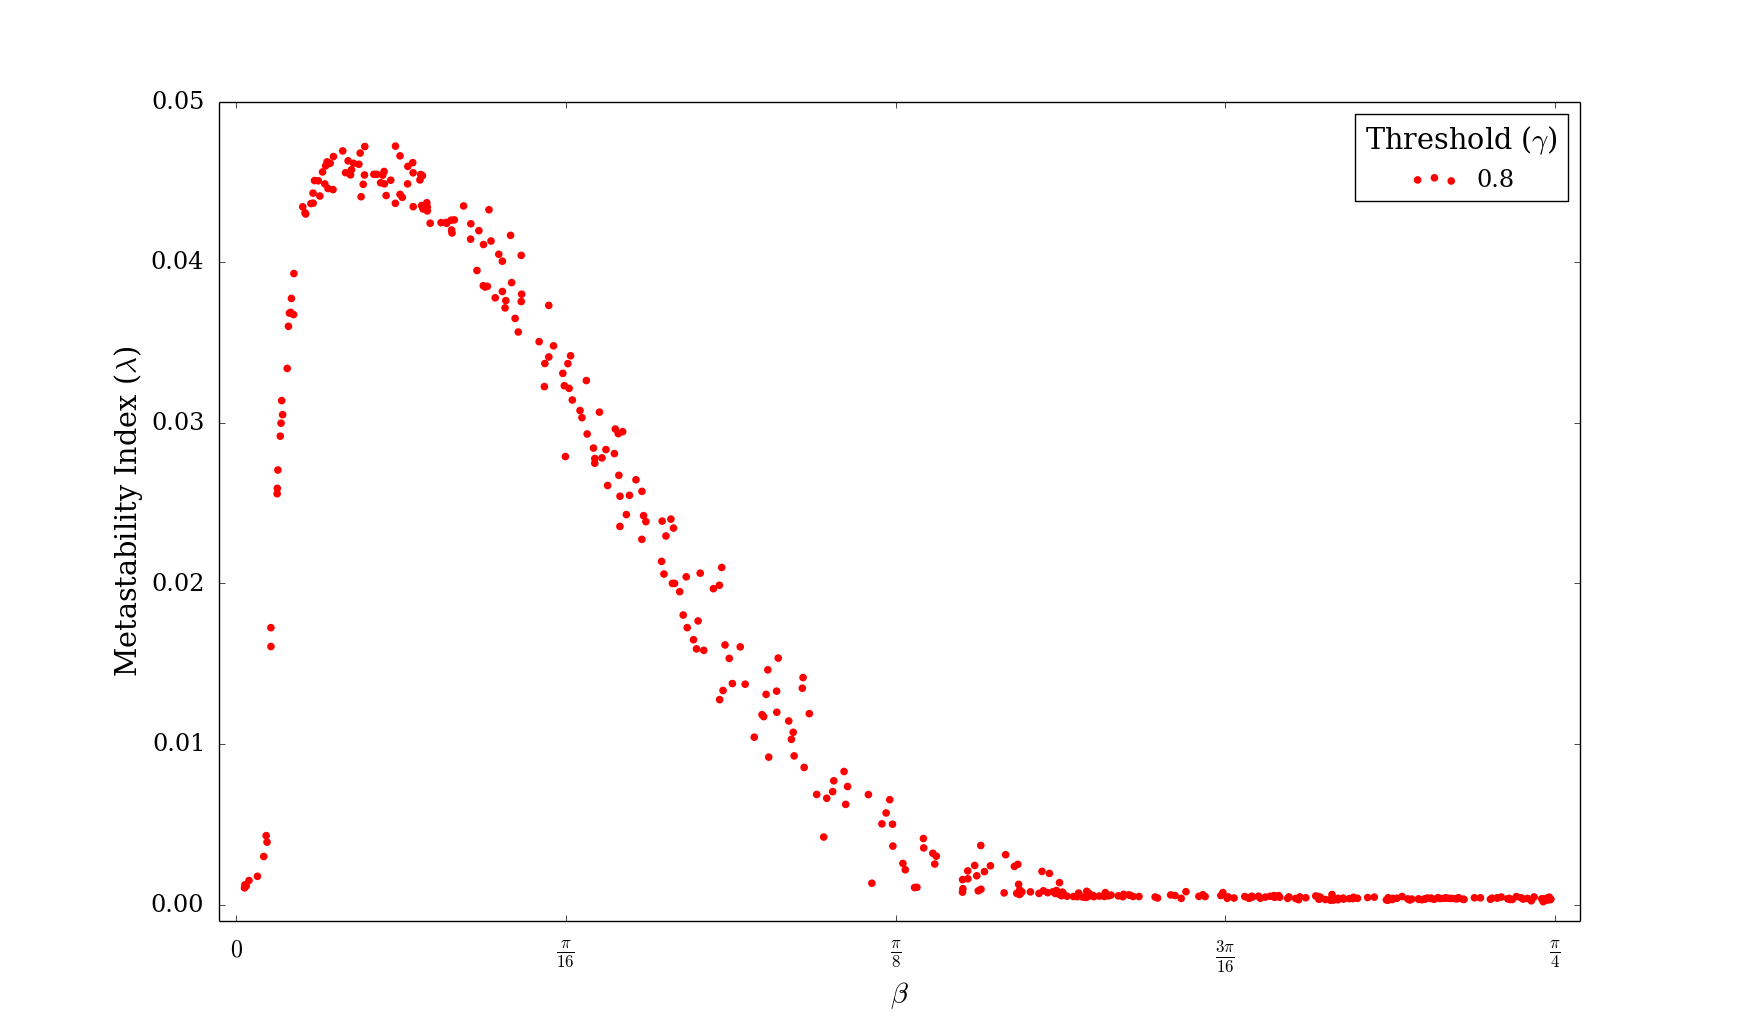
\includegraphics[scale = 0.35]{figures/lambda_vs_beta_orig}
\end{center}
\caption{
	Metastability Index ($\lambda$) vs $\beta$ for $0 \leq \beta \leq \frac{\pi}{4}$.
	\label{fig:lambda-vs-beta-orig}
}
\end{figure}

In order to gain a better picture of how $\beta$ and $\lambda$ interacted, we extended our $\beta$ range to cover the complete $0$ to $2\pi$ period. What we encountered was a second peak with an almost symmetrical shape as the peak in the original plot, centred around $\beta = 3.1$. The rest of the range remained flat, with $\lambda$ values close to zero, as depicted in Figure \ref{fig:lambda-vs-beta-ext}.

\begin{figure}[H]
\begin{center}
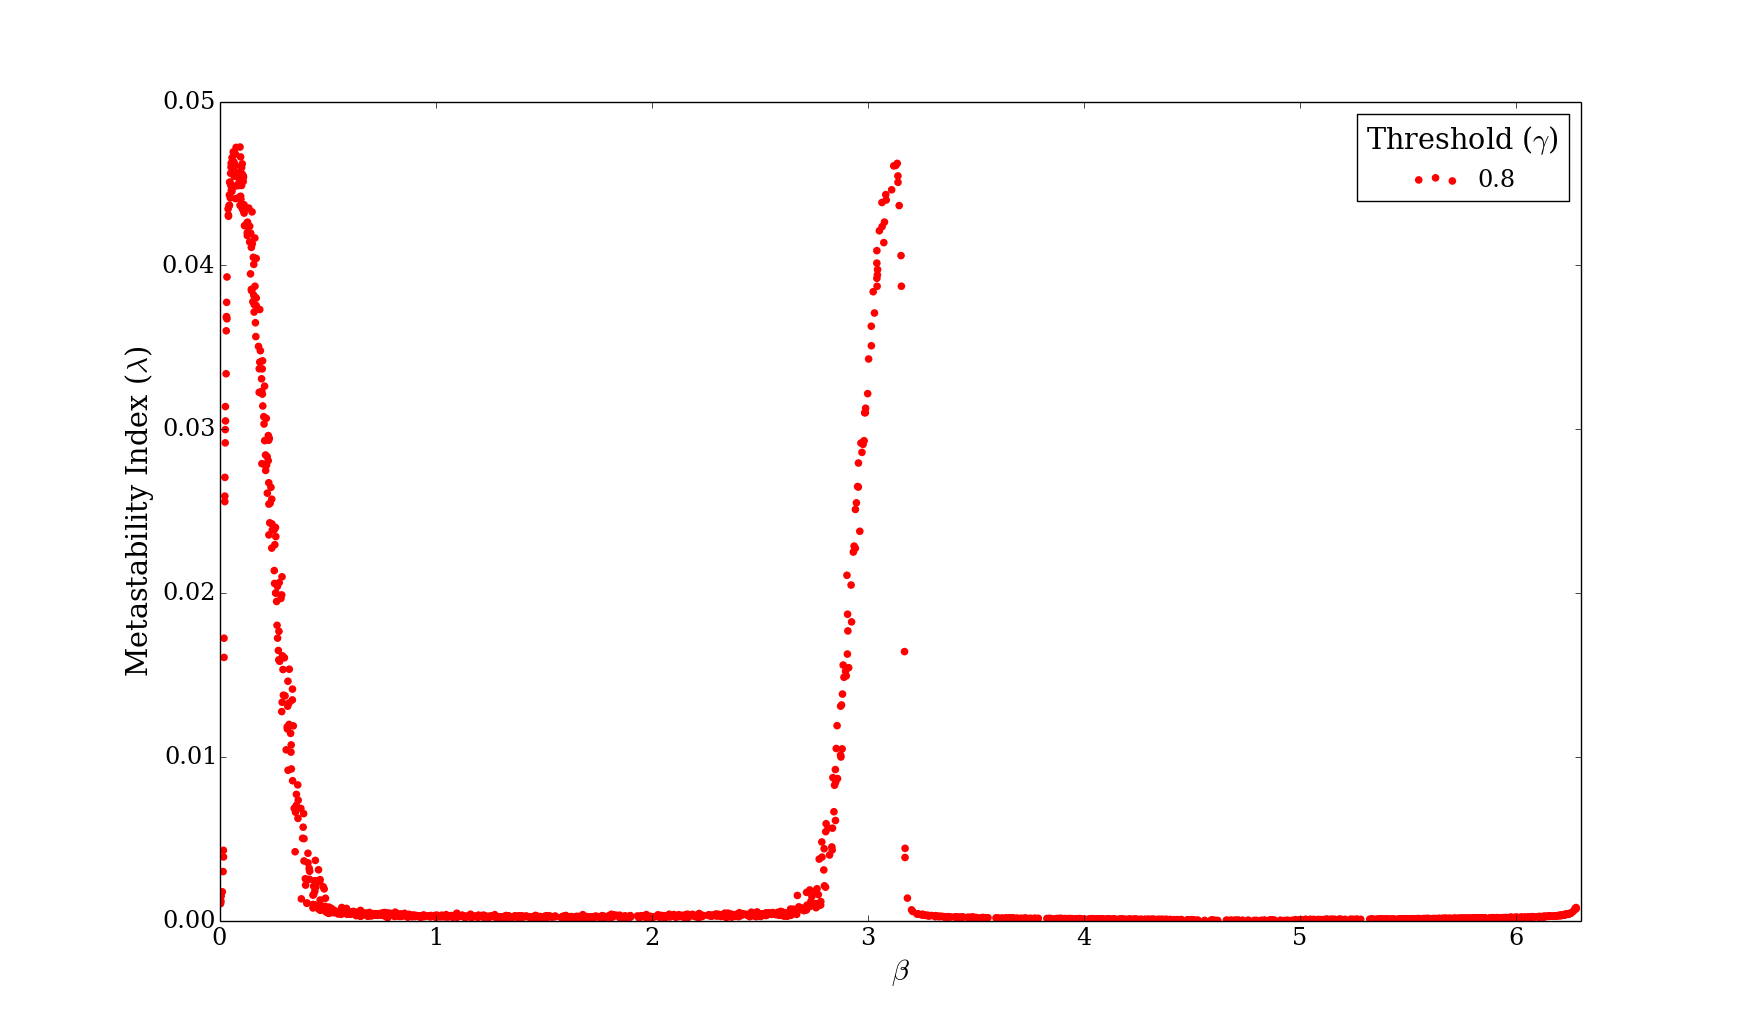
\includegraphics[scale = 0.35]{figures/lambda_vs_beta_ext}
\end{center}
\caption{
	Metastability Index ($\lambda$) vs $\beta$ for $0 \leq \beta \leq 2\pi$.
	\label{fig:lambda-vs-beta-ext}
}
\end{figure}

% -----------
% Chi vs Beta
% -----------
\subsubsection{Chimera Index ($\chi$) vs $\beta$}
\label{sec:app:osc:res:chi-v-beta}

The second correlation we examined corresponded again to a measure presented by Shanahan in \cite{Shanahan2010}. We plotted Shanahan's chimera index ($\chi$), as presented in Section \ref{sec:bg:chi}, versus $\beta$. Once again we started with $\beta$ ranging from $0$ to $\frac{\pi}{4}$, obtaining a result consistent with \cite{Shanahan2010}. As shown in Figure \ref{fig:chi-vs-beta-orig}, $\chi$ peaks at approximately $\beta = 0.08$, which falls in the range of $0.05 < \beta < 0.15$ found by Shanahan.

\begin{figure}[H]
\begin{center}
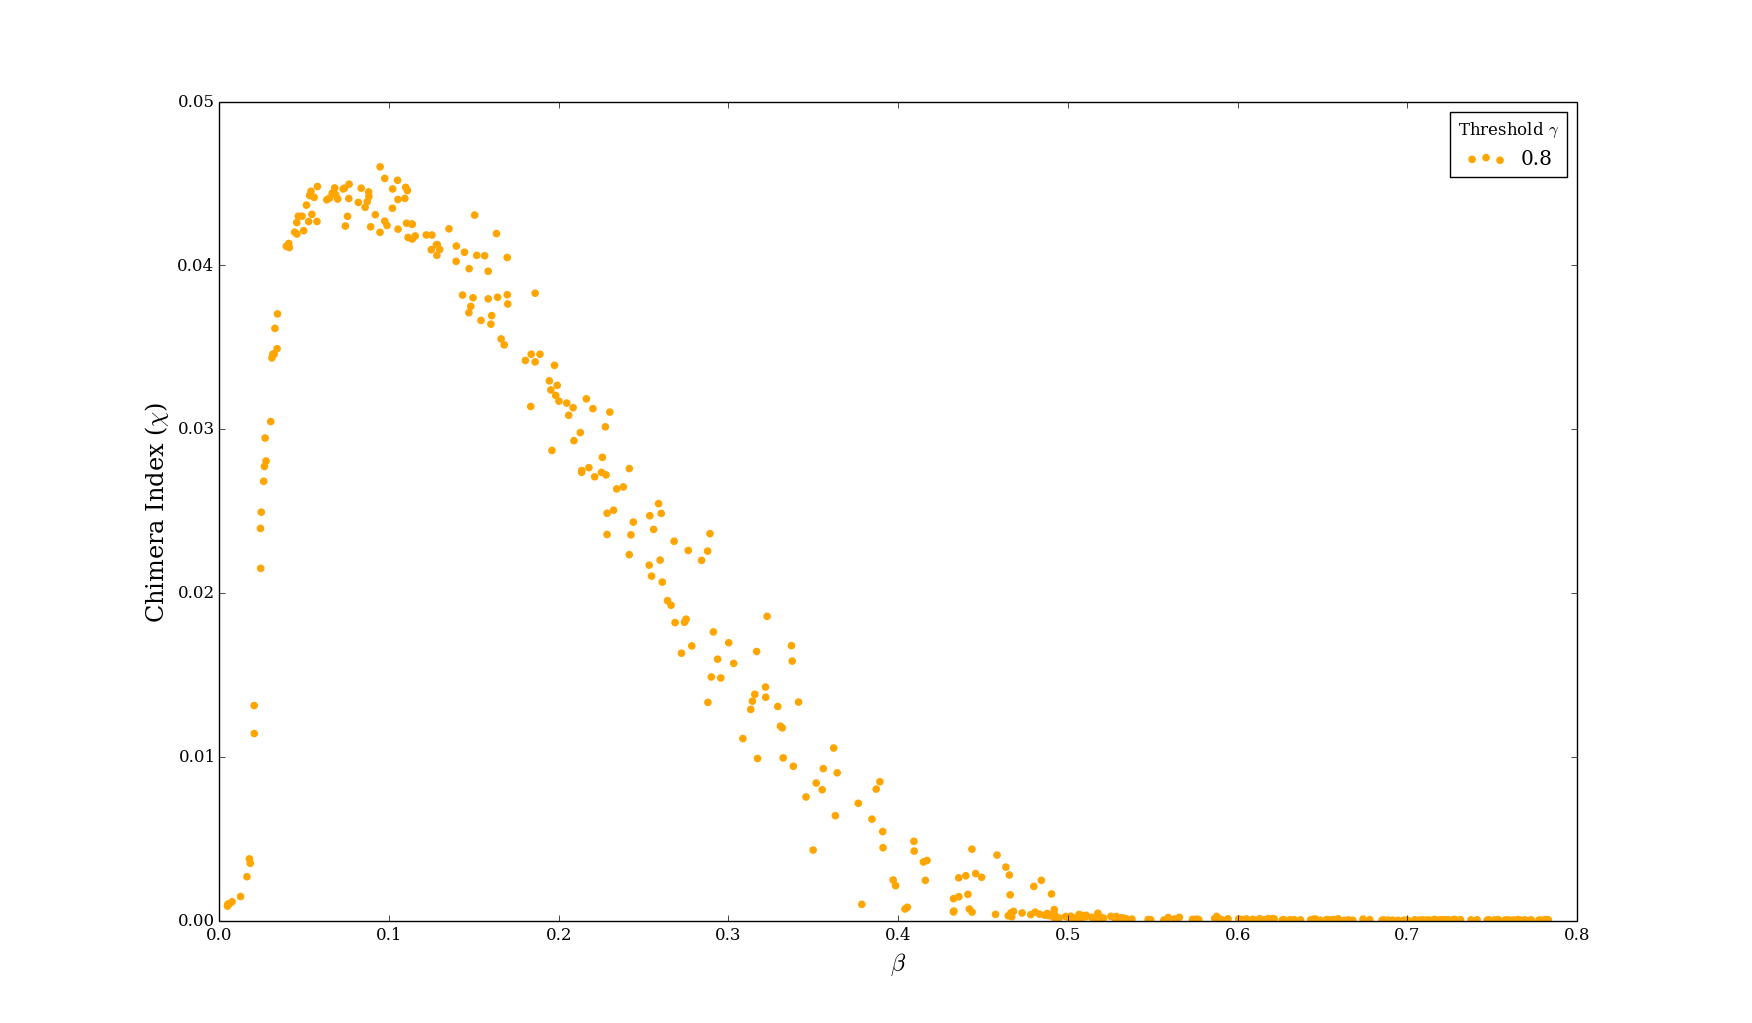
\includegraphics[scale = 0.35]{figures/chi_vs_beta_orig}
\end{center}
\caption{
	Chimera Index ($\chi$) vs $\beta$ for $0 \leq \beta \leq \frac{\pi}{4}$.
	\label{fig:chi-vs-beta-orig}
}
\end{figure}

As with the metastability index, we extended our $\beta$ range to cover $0 \leq \beta \leq 2\pi$. Again we encountered a second peak with an almost symmetrical shape as the one in the original plot. The new apex was also centred around $\beta = 3.1$, with the rest of the range remaining at $\chi$ values close to zero. This is depicted in Figure \ref{fig:chi-vs-beta-ext}.

\begin{figure}[H]
\begin{center}
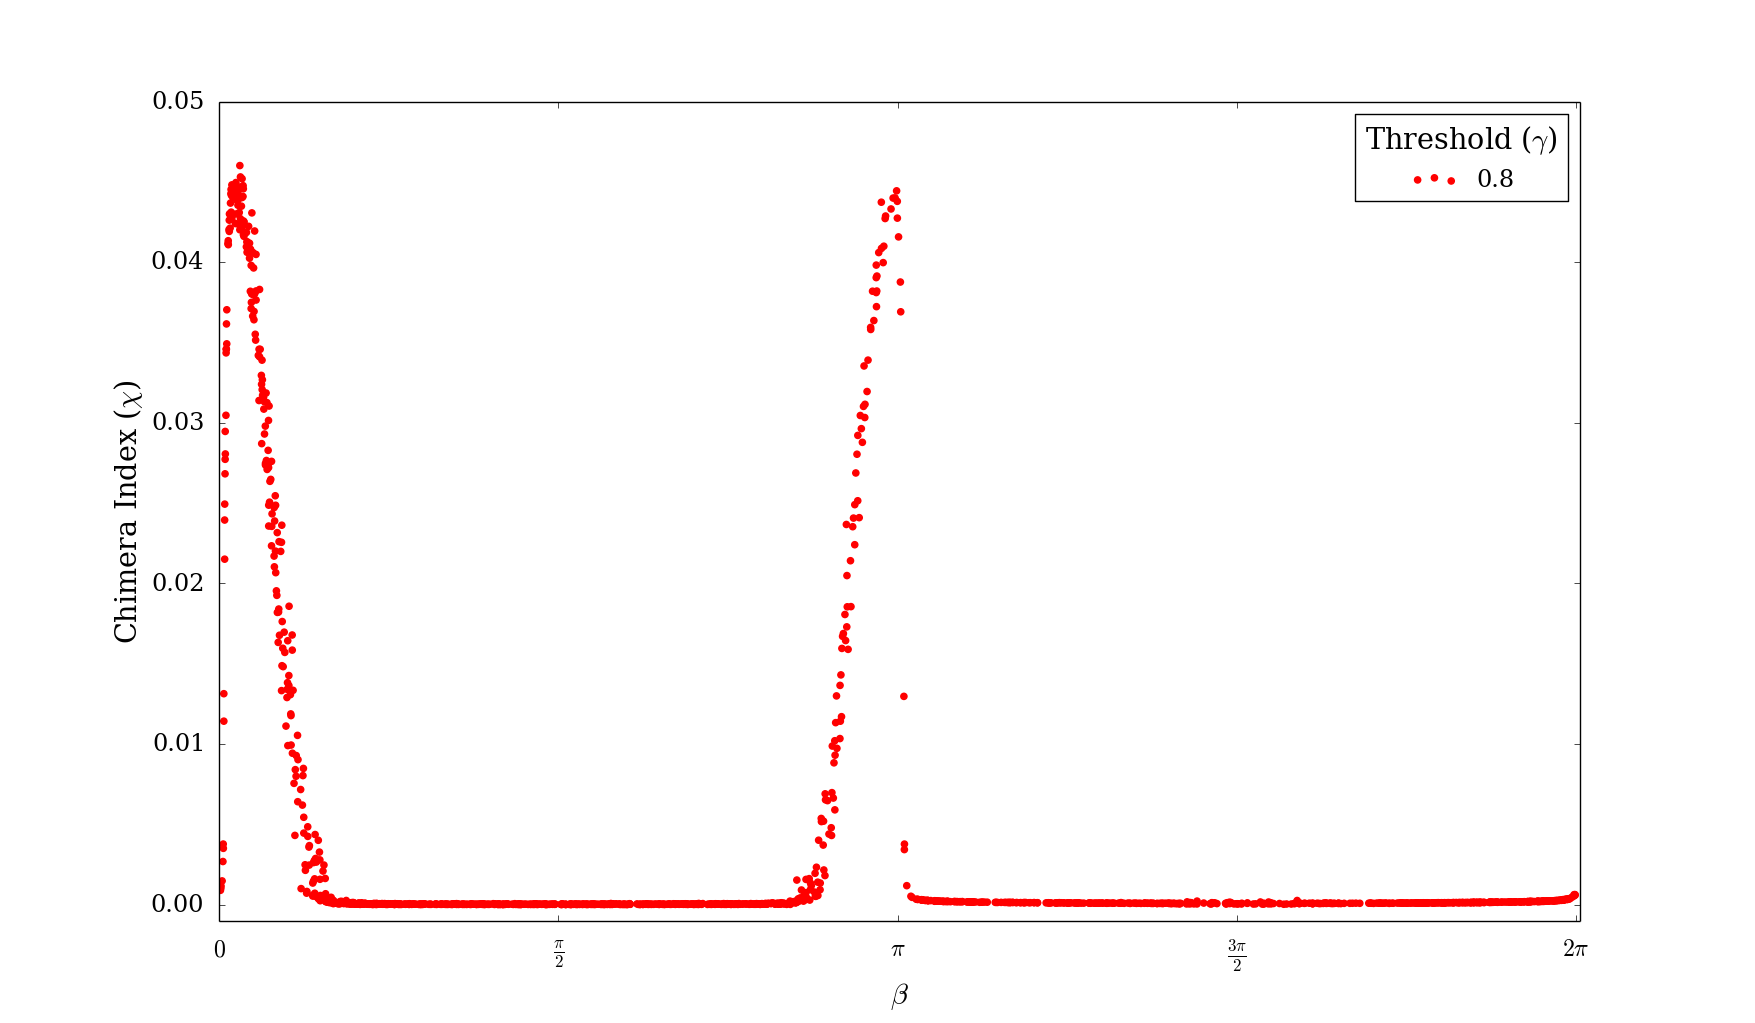
\includegraphics[scale = 0.35]{figures/chi_vs_beta_ext}
\caption{
	Chimera Index ($\chi$) vs $\beta$ for $0 \leq \beta \leq 2\pi$.
	\label{fig:chi-vs-beta-ext}
}
\end{center}
\end{figure}

\subsubsection{Global Synchrony vs $\beta$}
\label{sec:app:osc:res:sync-v-beta}

As synchrony is a key measure in determining the coalitions that are formed during each simulation, it was particularly important that our values for synchrony ($\psi$) and global synchrony ($\Psi$), as defined in Sections \ref{sec:bg:sync} and \ref{sec:bg:global-sync}, were behaving as expected. We thus examined the correlation between $\Psi$ and $\beta$. As shown in Figure \ref{fig:psi-vs-beta-orig}, our results were consistent with \cite{Shanahan2010}, with $\Psi$ tending towards full synchronisation across all communities for $\beta > \frac{\pi}{8}$.

\begin{figure}[H]
\begin{center}
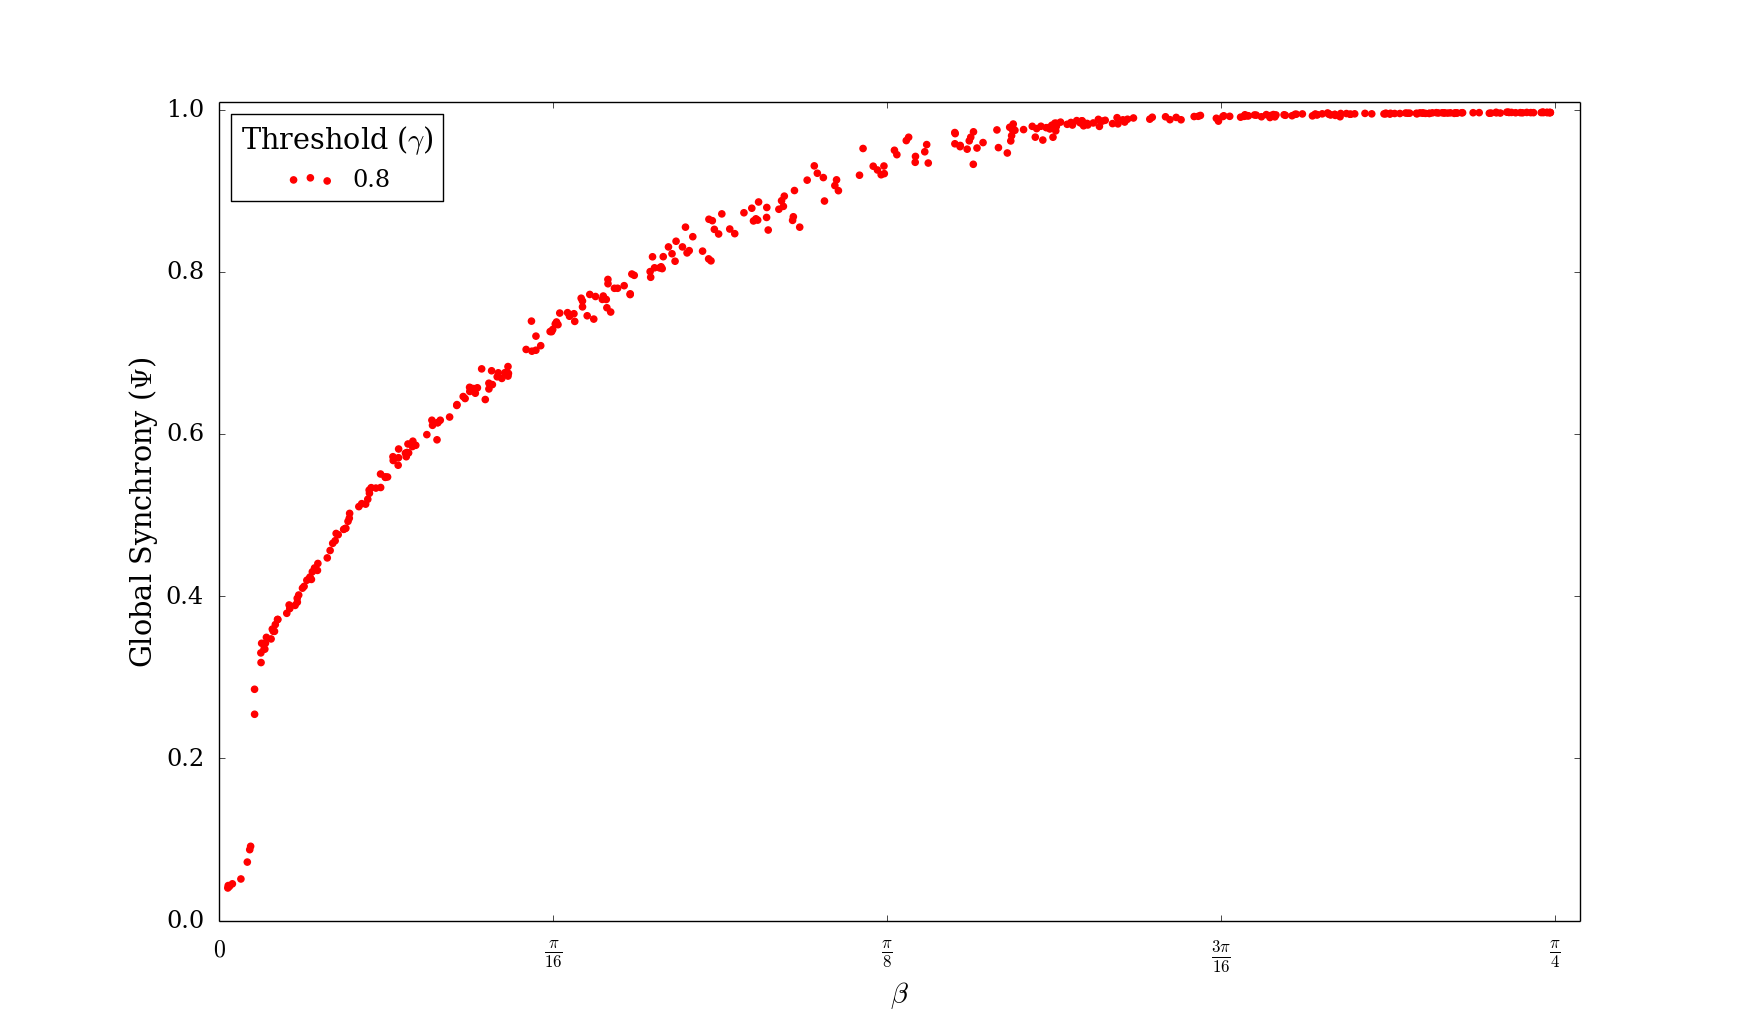
\includegraphics[scale = 0.35]{figures/psi_vs_beta_orig}
\caption{
	Global Synchrony ($\Psi$) vs $\beta$ for $0 \leq \beta \leq \frac{\pi}{4}$.
	\label{fig:psi-vs-beta-orig}
}
\end{center}
\end{figure}

To continue our analysis, we broadened our $\beta$ range to $0 < \beta < 2\pi$. As shown in Figure \ref{fig:psi-vs-beta-ext}, after $\beta = \frac{3\pi}{4}$ $\Psi$ starts declining and falls sharply at just under $\beta = \pi$. It then tends towards zero until $\frac{7\pi}{4}$, where it starts rising once more.

\begin{figure}[H]
\begin{center}
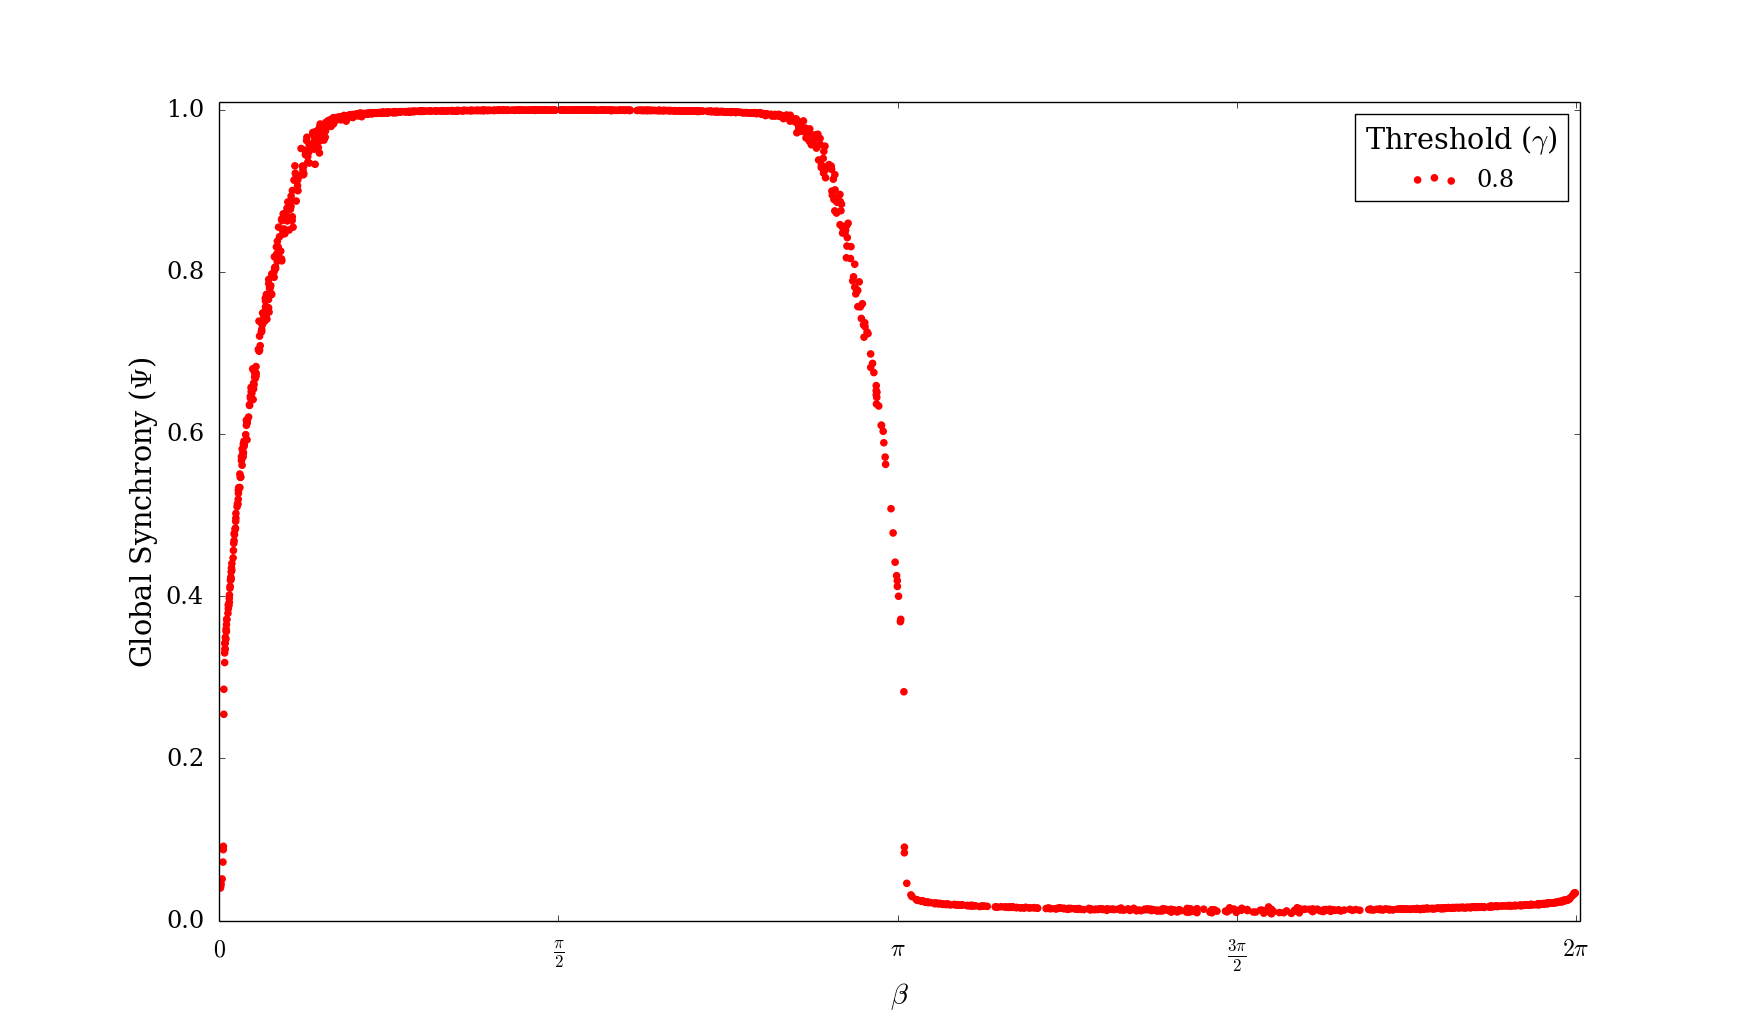
\includegraphics[scale = 0.35]{figures/psi_vs_beta_ext}
\caption{
	Global Synchrony ($\Psi$) vs $\beta$ for $0 \leq \beta \leq 2\pi$.
	\label{fig:psi-vs-beta-ext}
}
\end{center}
\end{figure}

% -------------------------
% Coalition Entropy vs Beta
% -------------------------
\subsubsection{Coalition Entropy ($H_C$) vs $\beta$}
\label{sec:app:osc:res:hc-v-beta}

A final correlation considered in \cite{Shanahan2010} that we examined in our project was the one between coalition entropy ($H_C$) and $\beta$. As shown in Figure \ref{fig:hc-vs-beta-orig}, $H_C$ peaks at a $\beta$ value of approximately $0.15$, which is consistent with \cite{Shanahan2010}. Figure \ref{fig:hc-vs-beta-orig} also presents the same broader spread of $H_C$ values around $0.35 < \beta < 0.5$ that can be seen in \cite{Shanahan2010}.

\begin{figure}[H]
\begin{center}
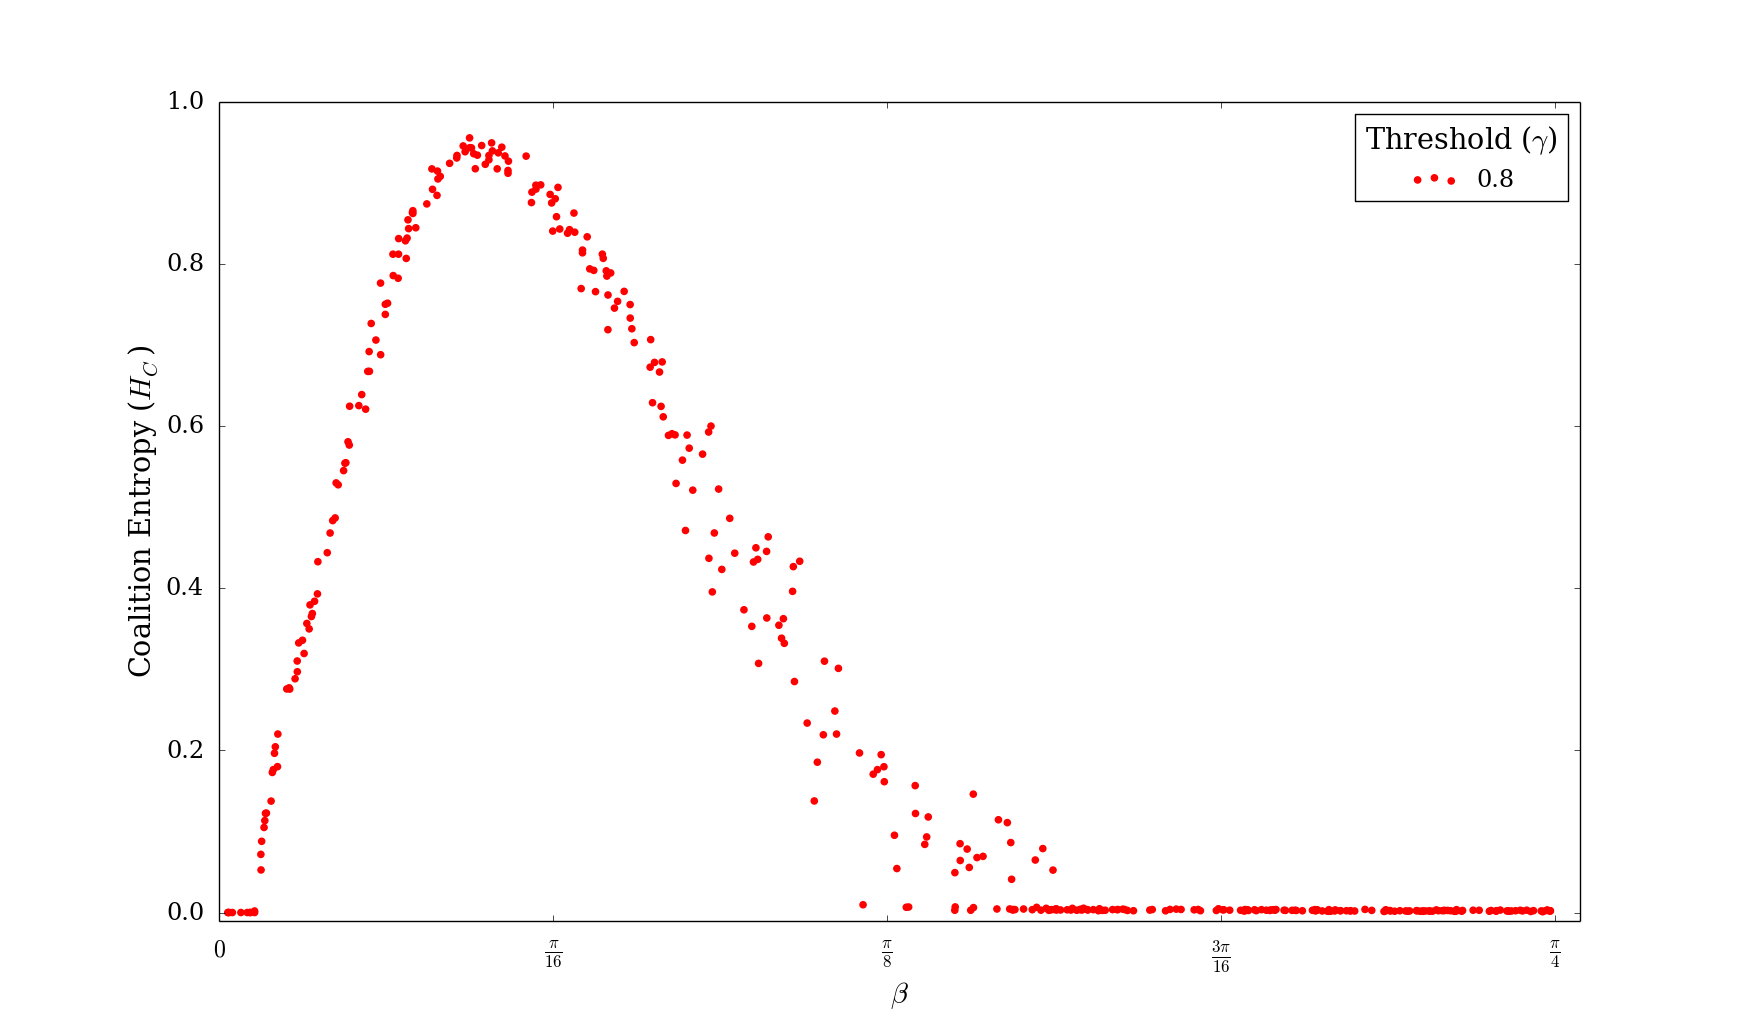
\includegraphics[scale = 0.35]{figures/hc_vs_beta_orig}
\caption{
	Coalition Entropy ($H_C$) vs $\beta$ for $0 \leq \beta \leq \frac{\pi}{4}$.
	\label{fig:hc-vs-beta-orig}
}
\end{center}
\end{figure}

When we examined the broader range of $0 \leq \beta \leq 2\pi$, we again saw a second symmetrical peak centred on $\beta = 3$, with $H_C$ tending towards zero for $\pi < \beta< 2\pi$.

\begin{figure}[H]
\begin{center}
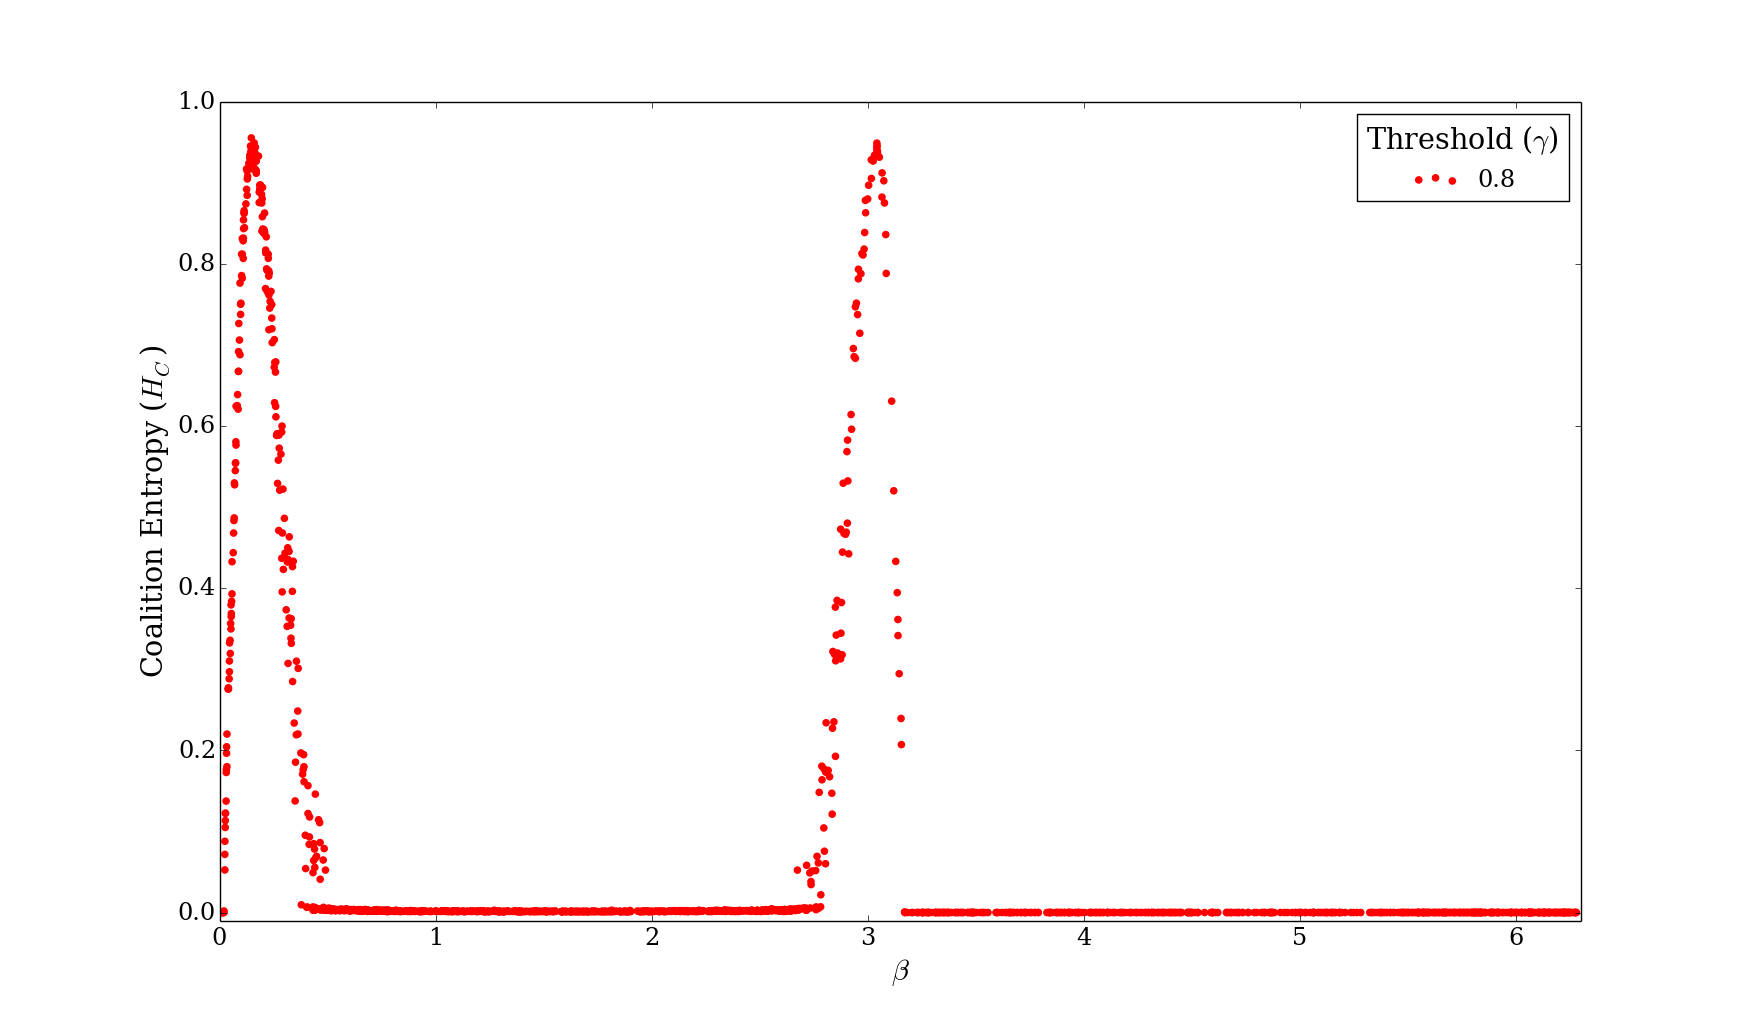
\includegraphics[scale = 0.35]{figures/hc_vs_beta_ext}
\caption{
	Coalition Entropy ($H_C$) vs $\beta$ for $0 \leq \beta \leq 2\pi$.
	\label{fig:hc-vs-beta-ext}
}
\end{center}
\end{figure}

We then extended our analysis to cover multiple thresholds ($\gamma$) for determining whether an oscillator was synchronised or not. As outlined in Section \ref{sec:osc:sims}, we applied thresholds $0.5$, $0.6$, $0.7$, $0.8$, and $0.9$ to each simulation.

As shown in Figure \ref{fig:hc-vs-beta-orig-multi} we can see that as $\gamma$ increases, the peak for $H_C$ shifts to the right and its maximum value decreases slightly. These values are highlighted in Table \ref{tab:max-hc-beta}. Additionally, we observed that the right skew of the peak clearly visible for $\gamma = 0.5$ diminishes as $\gamma$ increases and for $\gamma = 0.9$, the peak appears to be mostly symmetrical.

\begin{table}[ht]
\centering
\begin{tabular}{ c | c c }
\multicolumn{3}{c}{Maximum $H_C$} \\ [2mm]
$\gamma$ & $\beta$ & $H_C$\\
\hline
0.5 & 0.056 & 0.979 \\
0.6 & 0.075 & 0.974 \\
0.7 & 0.111 & 0.958 \\
0.8 & 0.147 & 0.954 \\
0.9 & 0.226 & 0.947 \\
\end{tabular}
\caption{
	The values of $\beta$ where coalition entropy ($H_C$) is maximised for each threshold ($\gamma$).
	\label{tab:max-hc-beta}
}
\end{table}

\begin{figure}[H]
\begin{center}
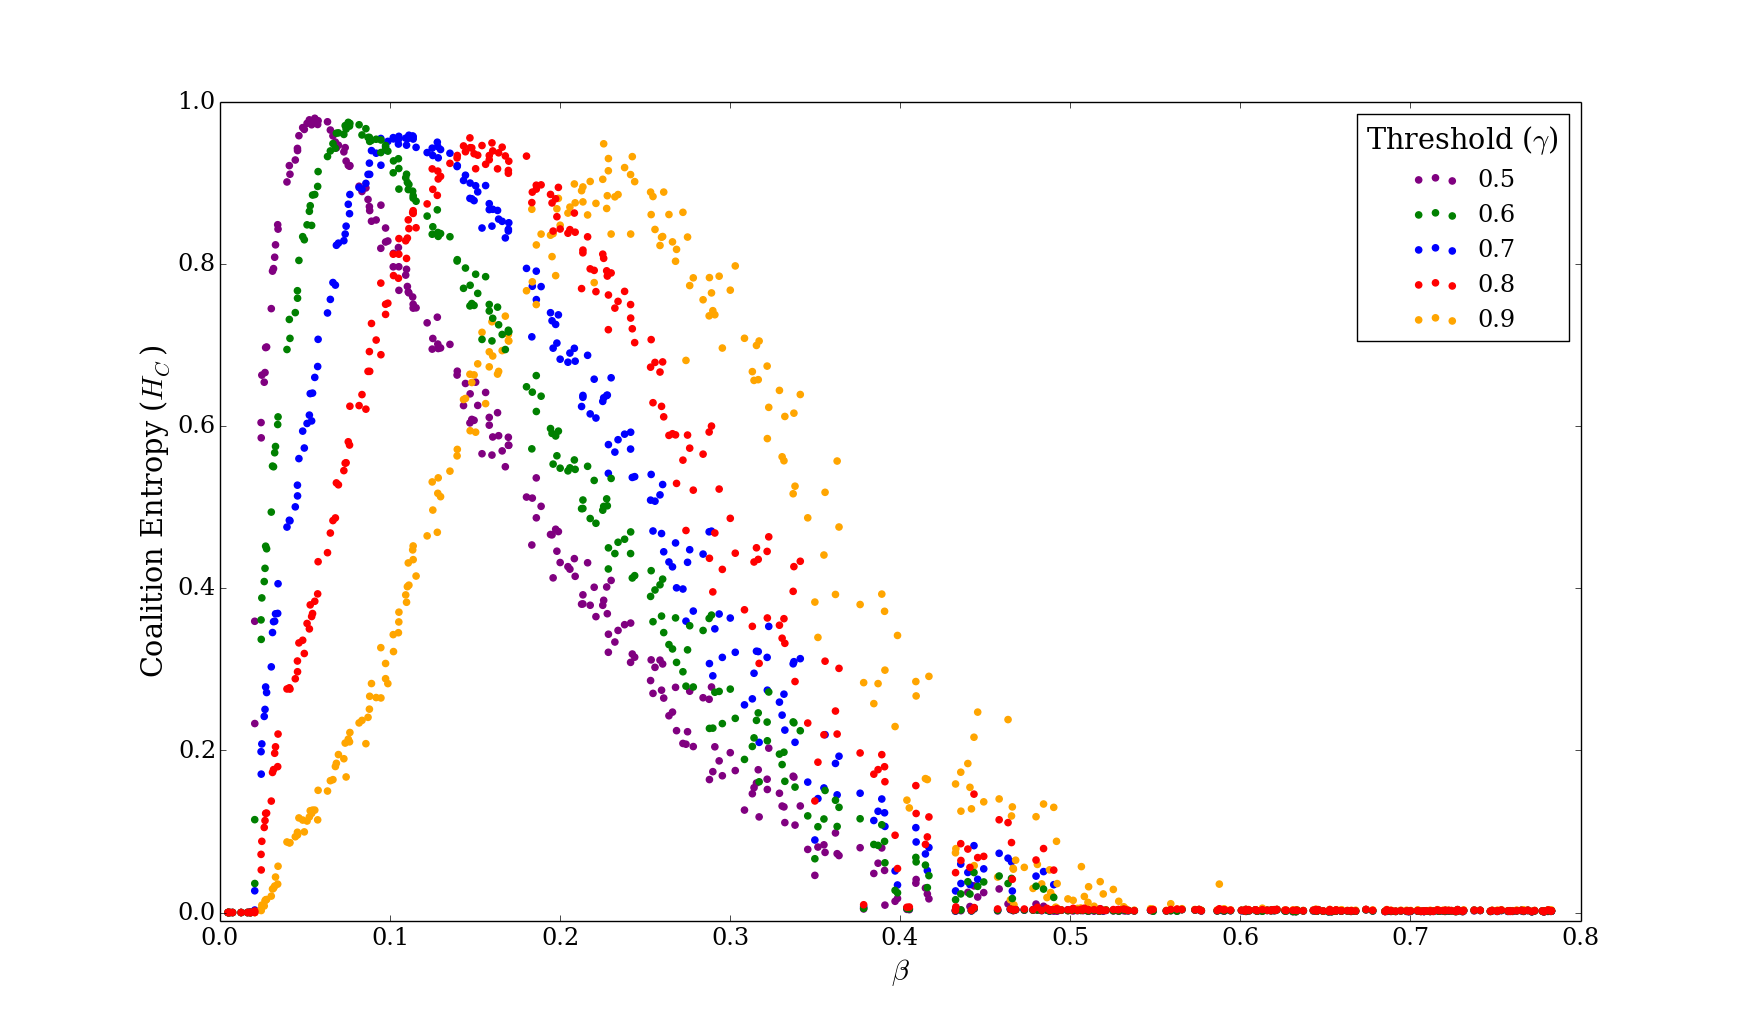
\includegraphics[scale = 0.35]{figures/hc_vs_beta_orig_multi}
\caption{
	Coalition Entropy ($H_C$) vs $\beta$ for $0 \leq \beta \leq \frac{\pi}{4}$ at multiple thresholds ($\gamma$).
	\label{fig:hc-vs-beta-orig-multi}
}
\end{center}
\end{figure}

When we extended our $\beta$ range to $0 \leq \beta \leq 2\pi$, we observed the same symmetrical peak for each threshold as previously observed for $\gamma = 0.8$. Similarly, for all thresholds, $H_C$ tends towards zero for $\pi < \beta< 2\pi$.

\begin{figure}[H]
\begin{center}
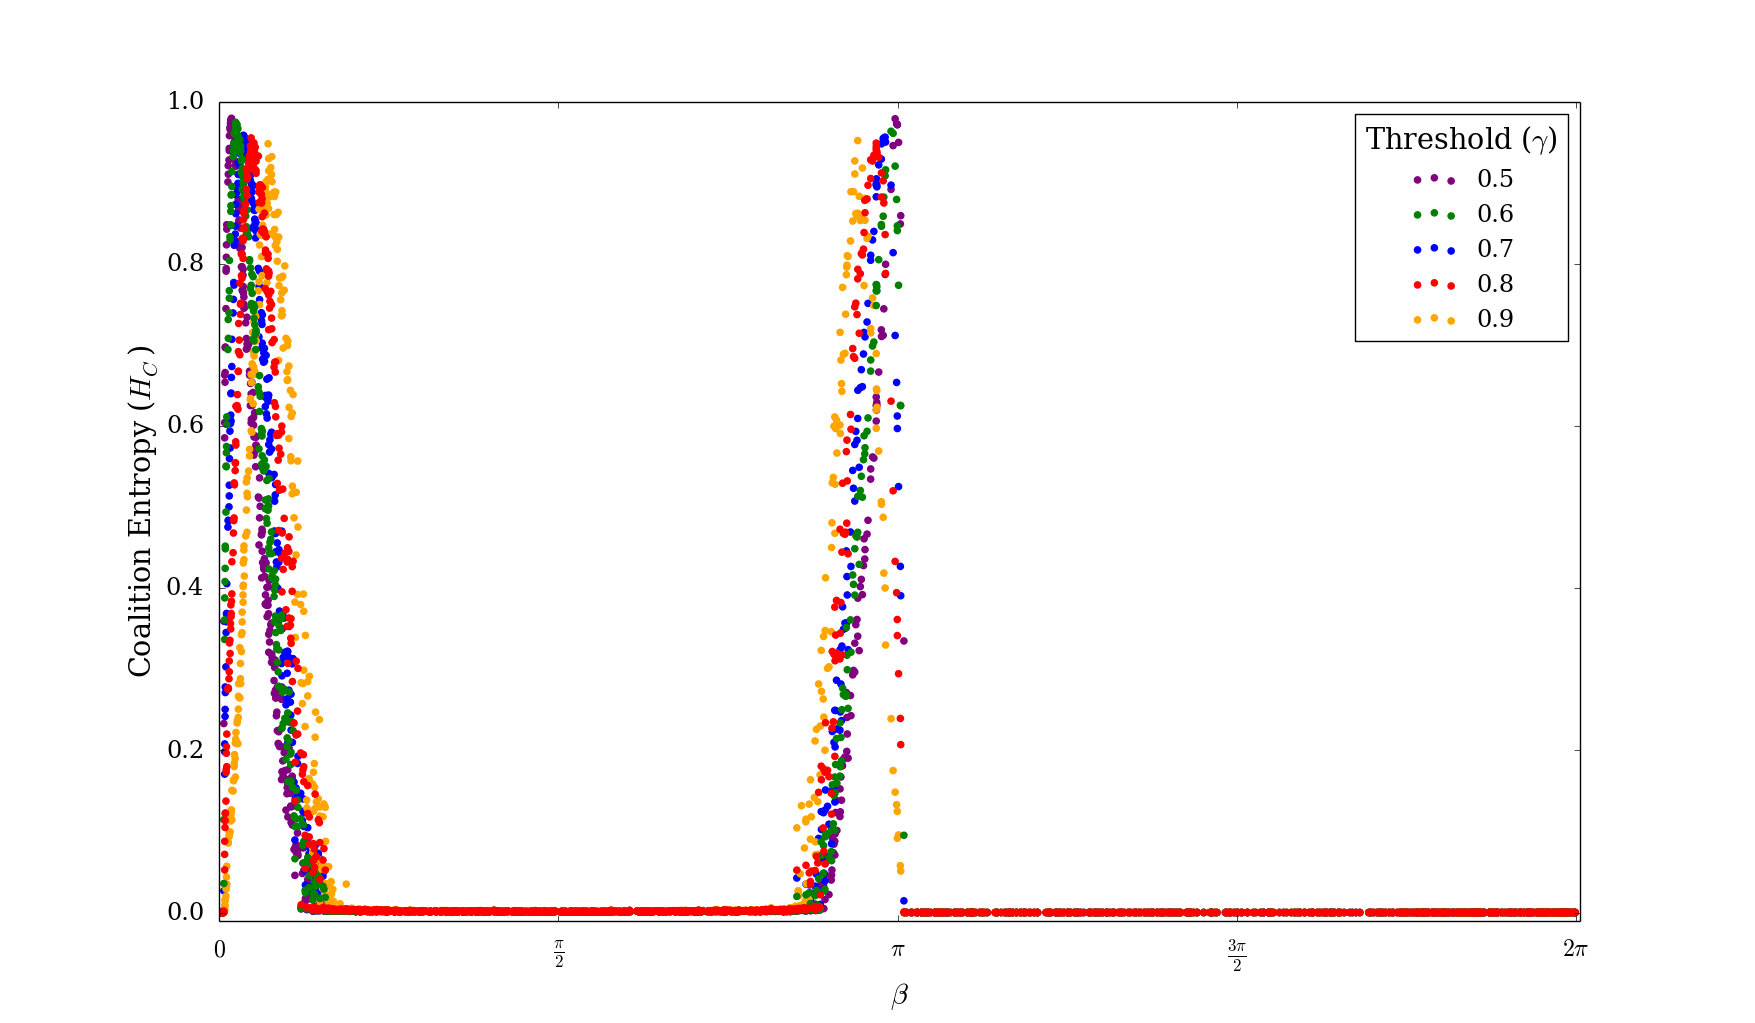
\includegraphics[scale = 0.35]{figures/hc_vs_beta_ext_multi}
\caption{
	Coalition Entropy ($H_C$) vs $\beta$ for $0 \leq \beta \leq 2\pi$ at multiple thresholds ($\gamma$).
	\label{fig:hc-vs-beta-ext-multi}
}
\end{center}
\end{figure}

% -----------
% Phi vs Beta
% -----------
\subsubsection{Empirical Integrated Information ($\Phi_{E}$) vs $\beta$}
\label{sec:app:osc:res:phi-v-beta}

Having completed an analysis of the relationships considered by Shanahan in \cite{Shanahan2010}, we started analysing comparable correlations using our measures of integrated information. To begin with, we considered empirical integrated information ($\Phi_{E}$), as defined in Section \ref{II}, and plotted it against $\beta$.

Figure \ref{fig:phi-vs-beta-orig} shows the correlation between $\Phi_{E}$ and $\beta$ for a range of $0 \leq \beta \leq \frac{\pi}{4}$. We observe that the peak reaches its apex at $\beta \approx 0.16$. This closely follows what we found for $H_C$ when plotted against $\beta$, where $H_C$ reached a maximum at $\beta \approx 0.15$. It is worth noting, however, that the peak for $\Phi_{E}$ versus $\beta$ is narrower than that of $H_C$ versus $\beta$, and that the former, before it starts rising at $\beta \approx 0.07$, presents a dip, where $\Phi_{E}$ reaches values of down to approximately $-0.06$. For $H_C$, this is not possible, given that by definition it cannot take negative values. Additionally, we can see that from $\beta \approx 0.27$ onwards, the value for $\Phi_{E}$ stabilises at close to zero. 

\begin{figure}[H]
\begin{center}
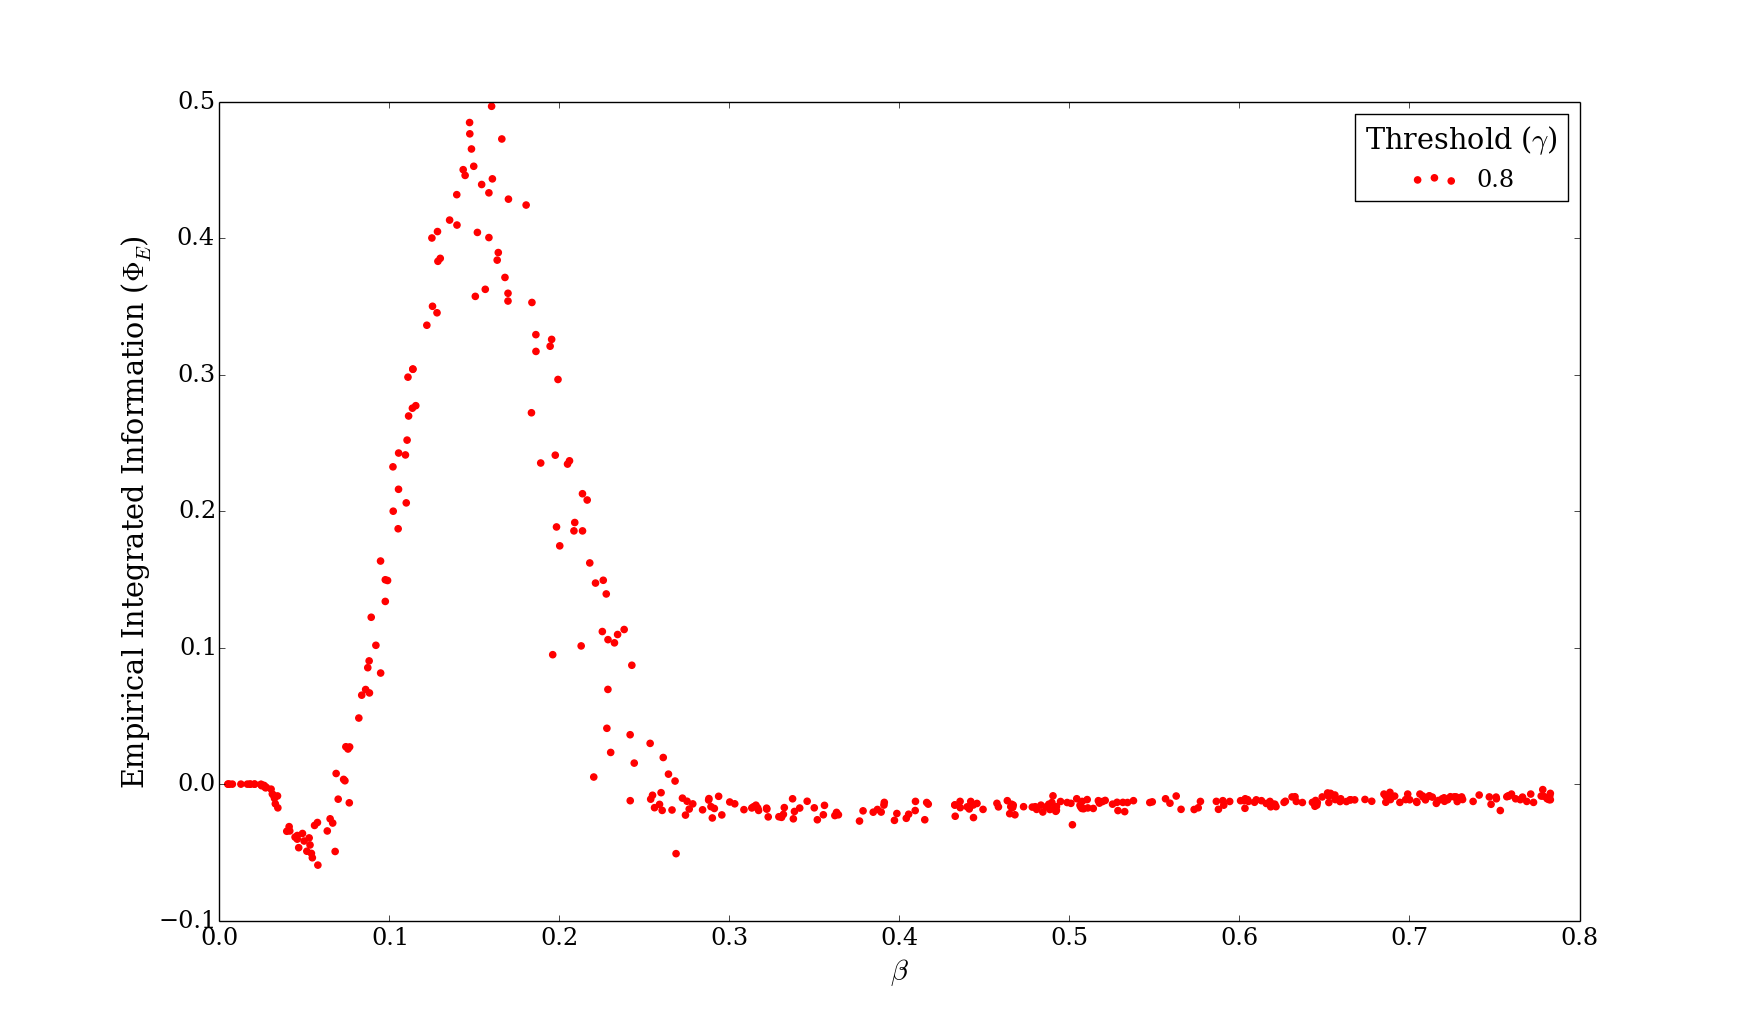
\includegraphics[scale = 0.35]{figures/phi_vs_beta_orig}
\caption{
	Empirical Integrated Information ($\Phi_E$) vs $\beta$ for $0 \leq \beta \leq \frac{\pi}{4}$.
	\label{fig:phi-vs-beta-orig}
}
\end{center}
\end{figure}

As we the previous measures plotted against $\beta$, we extended the range to $0 \leq \beta \leq 2\pi$. Once more we found a symmetrical peak centred around $\beta \approx 3.1$, with $\Phi_E$ stabilising at around zero for values greater than $\beta \approx 3.17$. This depicted in Figure \ref{fig:phi-vs-beta-ext}.

\begin{figure}[H]
\begin{center}
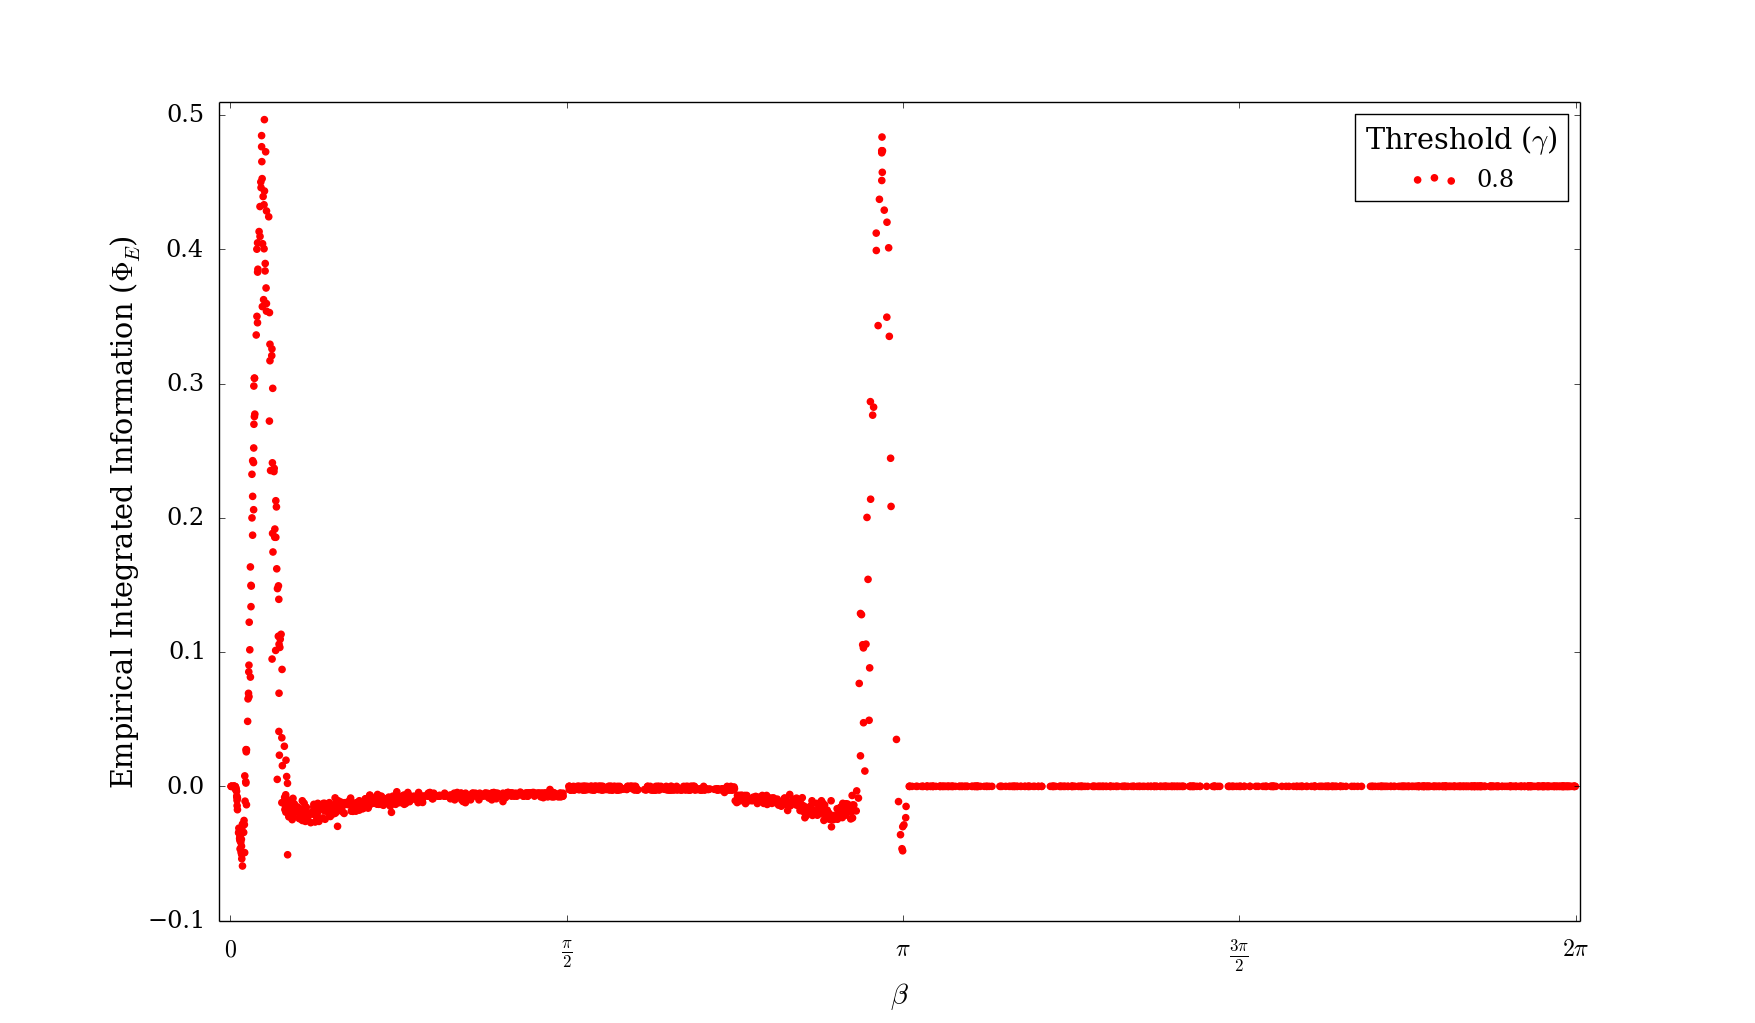
\includegraphics[scale = 0.35]{figures/phi_vs_beta_ext}
\caption{
	Empirical Integrated Information ($\Phi_E$) vs $\beta$ for $0 \leq \beta \leq 2\pi$.
	\label{fig:phi-vs-beta-ext}
}
\end{center}
\end{figure}


When considering multiple thresholds ($\gamma$), we observed a behaviour similar to the one for coalition entropy described in Section \ref{sec:app:osc:res:hc-v-beta}. As $\gamma$ increases, the value of $\beta$ corresponding to the maximum value of $\Phi_E$ also increases. However, the maximum value of $\Phi_E$ doesn't necessarily decrease. It decreases from $\gamma = 0.5$ to $\gamma = 0.7$, but then increases from $\gamma = 0.7$ to $\gamma = 0.9$. This shift and change in maximum $\Phi_E$ can be observed in Figure \ref{fig:phi-vs-beta-orig-multi} and is summarised in Table \ref{tab:max-phi-beta}.

\begin{table}[ht]
\centering
\begin{tabular}{ c | c c }
\multicolumn{3}{c}{Maximum $\Phi_E$} \\ [2mm]
$\gamma$ & $\beta$ & $\Phi_E$\\
\hline
0.5 & 0.056 & 0.546 \\
0.6 & 0.082 & 0.525 \\
0.7 & 0.114 & 0.465 \\
0.8 & 0.160 & 0.500 \\
0.9 & 0.238 & 0.632 \\
\end{tabular}
\caption{
	The values of $\beta$ where empirical integrated information ($\Phi_E$) is maximised for each threshold ($\gamma$).
	\label{tab:max-phi-beta}
}
\end{table}

\begin{figure}[H]
\begin{center}
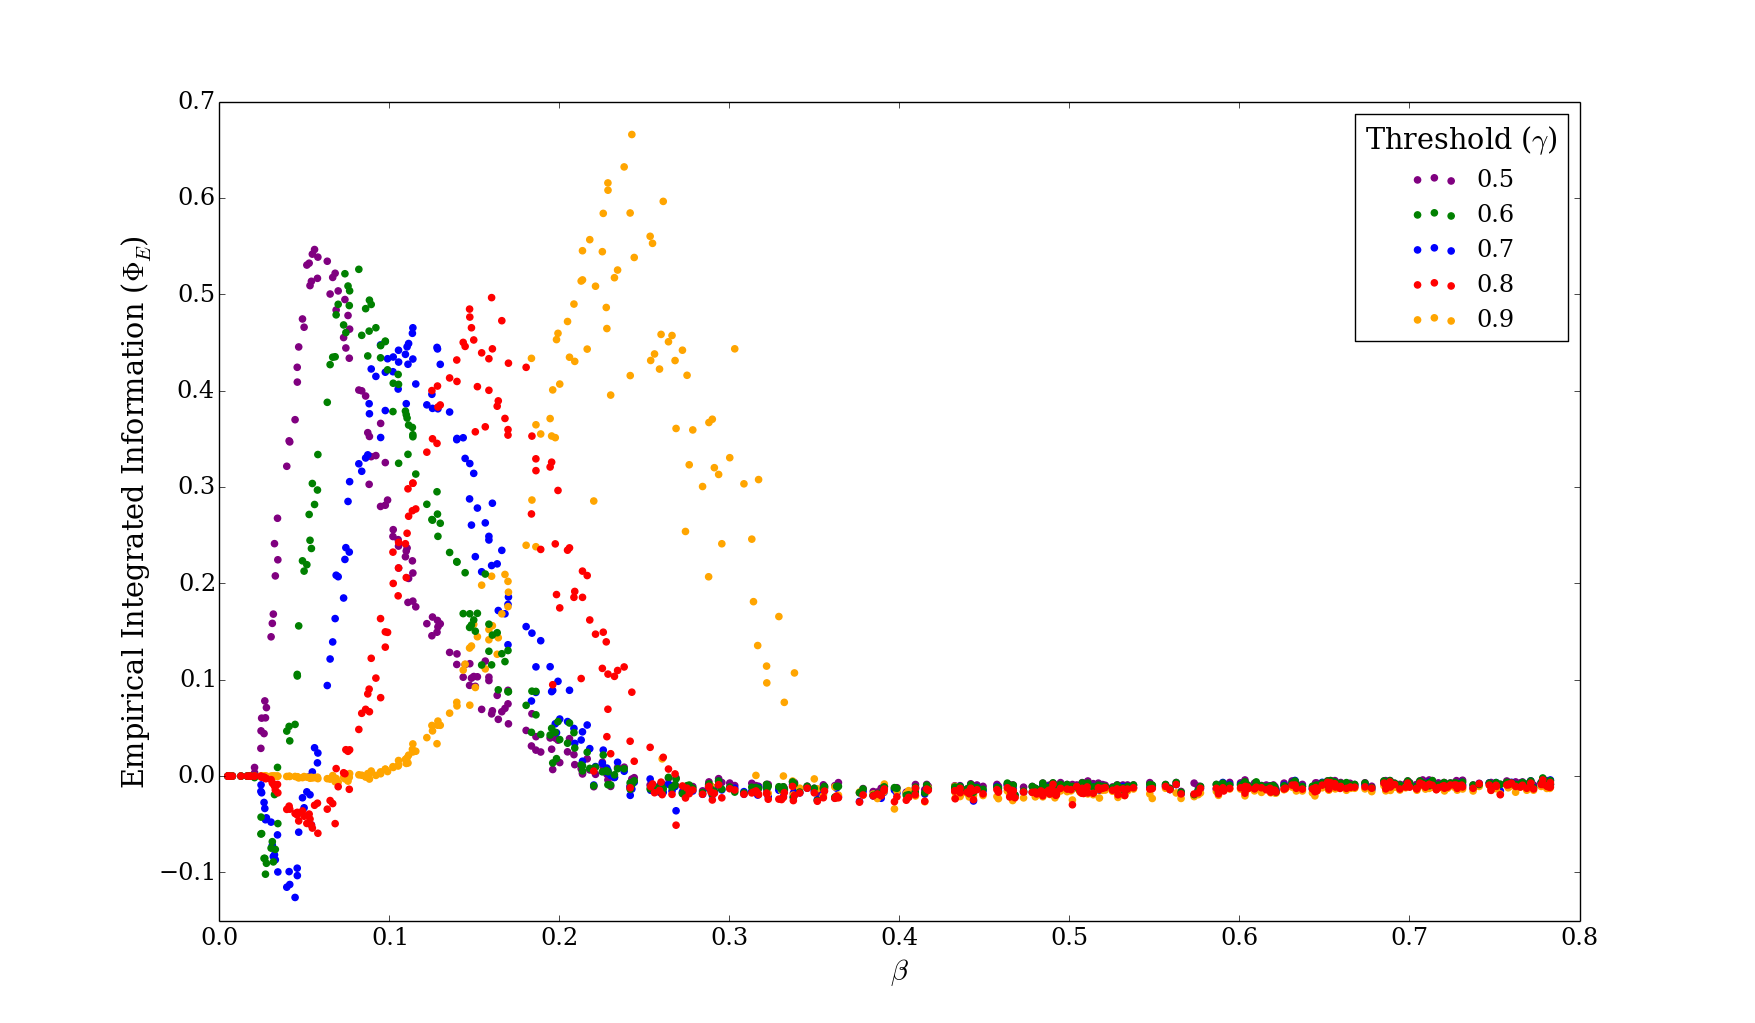
\includegraphics[scale = 0.35]{figures/phi_vs_beta_orig_multi}
\caption{
	Empirical Integrated Information ($\Phi_E$) vs $\beta$ for $0 \leq \beta \leq \frac{\pi}{4}$ at multiple thresholds ($\gamma$).
	\label{fig:phi-vs-beta-orig-multi}
}
\end{center}
\end{figure}

With an extended $\beta$ range, all the multiple thresholds exhibit the same behaviour, with a symmetrical peak appearing at $\beta \approx 3.1$. This can be observed in Figure \ref{fig:phi-vs-beta-ext-multi}.

\begin{figure}[H]
\begin{center}
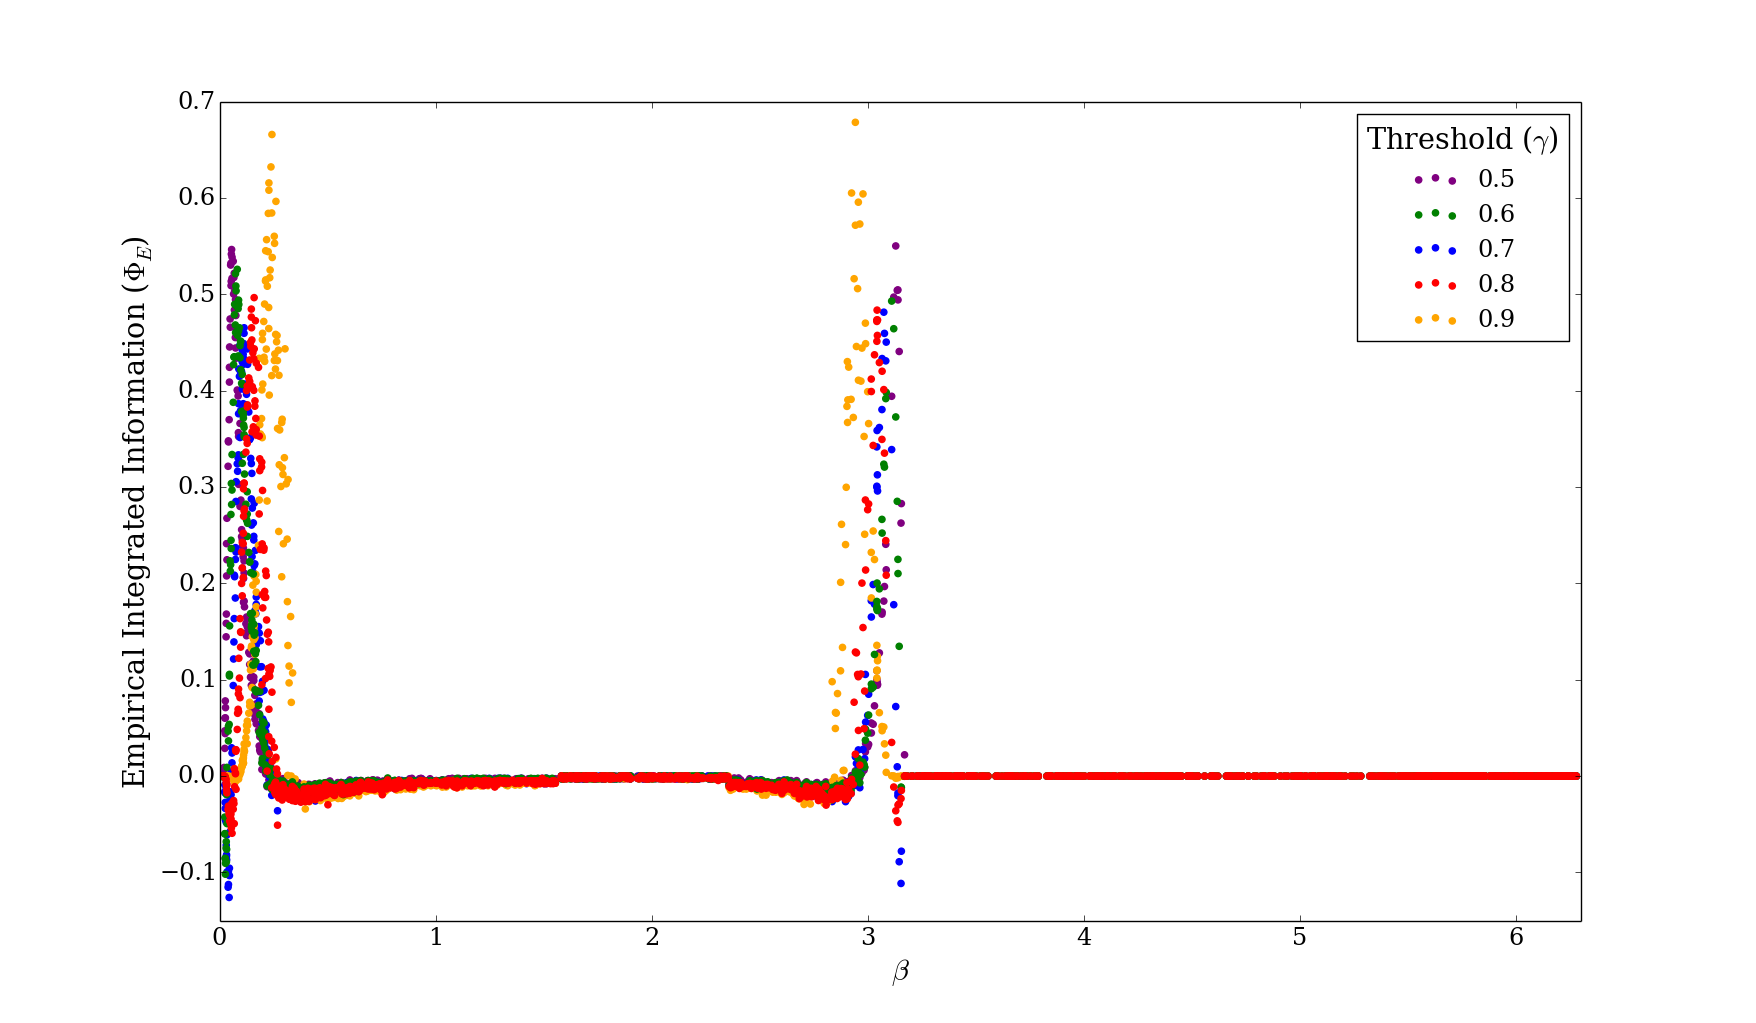
\includegraphics[scale = 0.35]{figures/phi_vs_beta_ext_multi}
\caption{
	Empirical Integrated Information ($\Phi_E$) vs $\beta$ for $0 \leq \beta \leq 2\pi$ at multiple thresholds ($\gamma$).
	\label{fig:phi-vs-beta-ext-multi}
}
\end{center}
\end{figure}


% -----------------
% Phi Tilde vs Beta
% -----------------
\subsubsection{Empirical Integrated Information Tilde ($\widetilde{\Phi}_{E}$) vs $\beta$}
\label{sec:app:osc:res:phi-tilde-v-beta}

We observed comparable results when analysing the relationship between the alternative measure for empirical integrated information, $\widetilde{\Phi}_{E}$, as defined in Section \ref{II}, and $\beta$. When plotting only $\gamma = 0.8$ in Figures \ref{fig:phi-tilde-vs-beta-orig} and \ref{fig:phi-tilde-vs-beta-ext}, we can clearly observe the same peak centred around $\beta \approx 0.15$, with its symmetrical peak on $\beta \approx 3.1$. When plotting multiple thresholds in Figures \ref{fig:phi-tilde-vs-beta-orig-multi} and \ref{fig:phi-tilde-vs-beta-ext-multi}, we observe the same shift and change in maximum $\widetilde{\Phi}_{E}$ values observed in section \ref{sec:app:osc:res:phi-v-beta}.

\begin{figure}[H] 
	\label{fig:phi-tilde-vs-beta-all} 
	\begin{minipage}[b]{0.5\linewidth}
		\begin{center}
		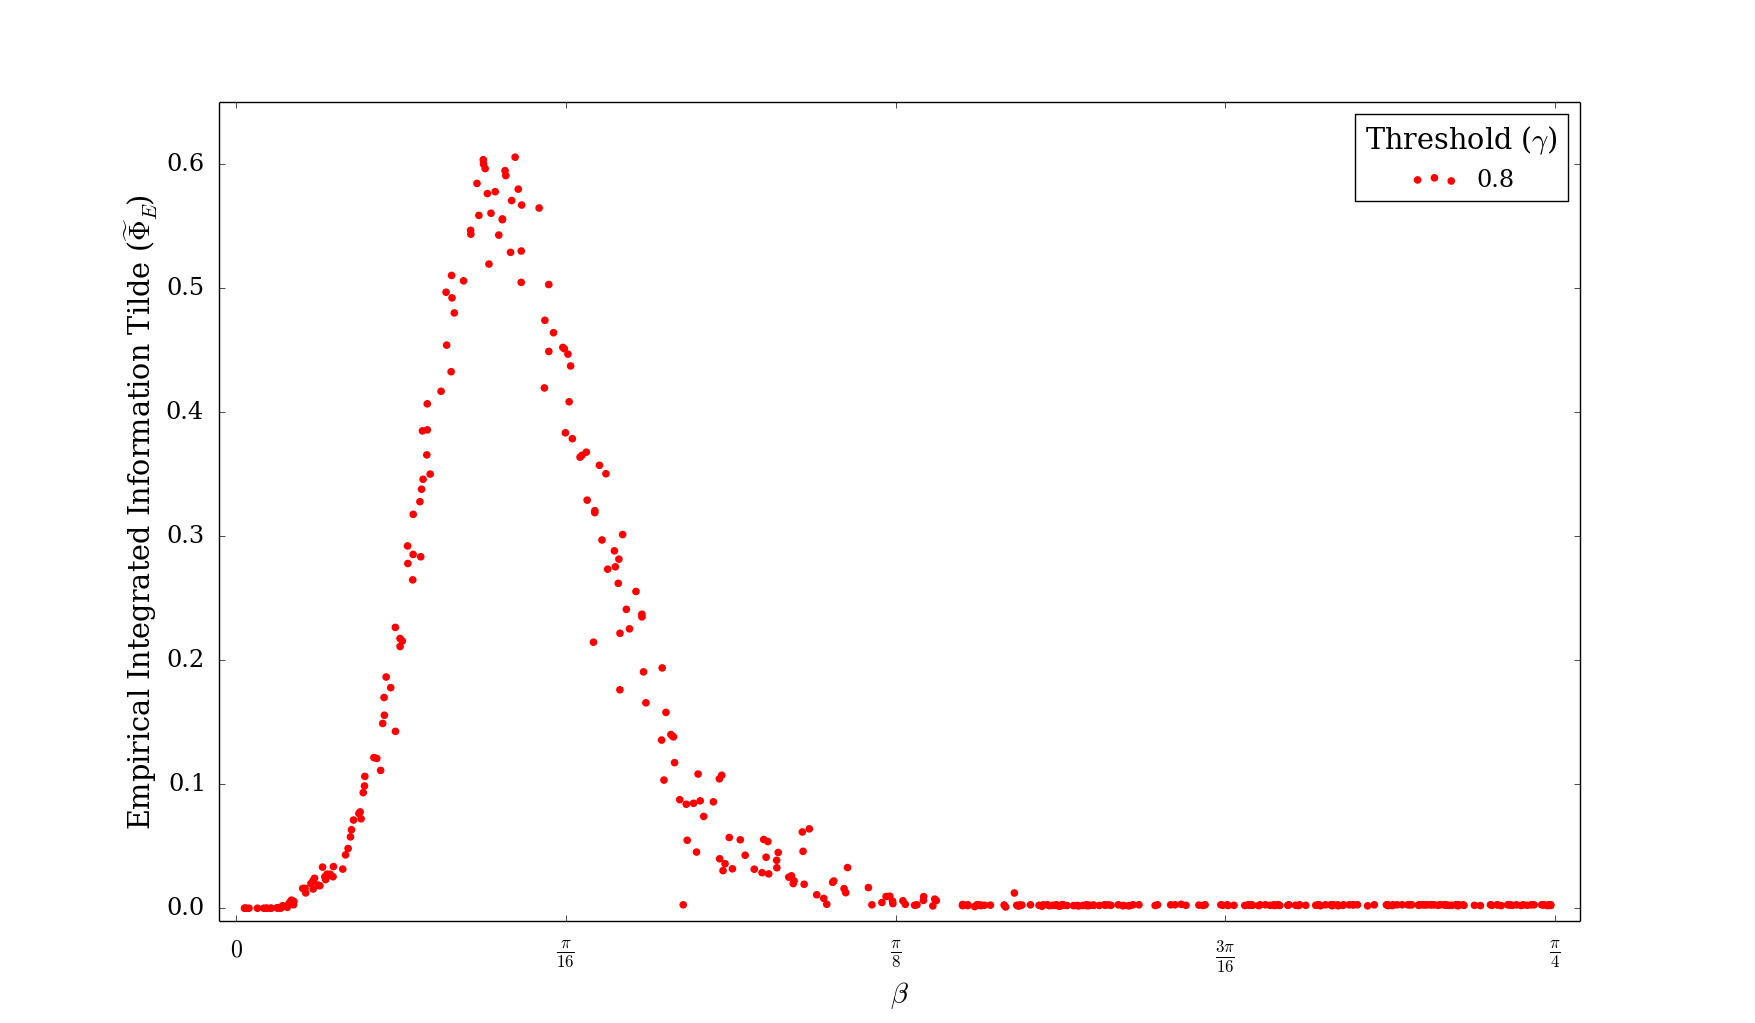
\includegraphics[scale = 0.2]{figures/phi_tilde_vs_beta_orig}
		\caption{
				$\widetilde{\Phi}_E$ vs $\beta$ for $0 \leq \beta \leq \frac{\pi}{4}$.
			\label{fig:phi-tilde-vs-beta-orig}
		}
		\end{center}
		\vspace{4ex}
	\end{minipage}
	\begin{minipage}[b]{0.5\linewidth}
		\begin{center}
		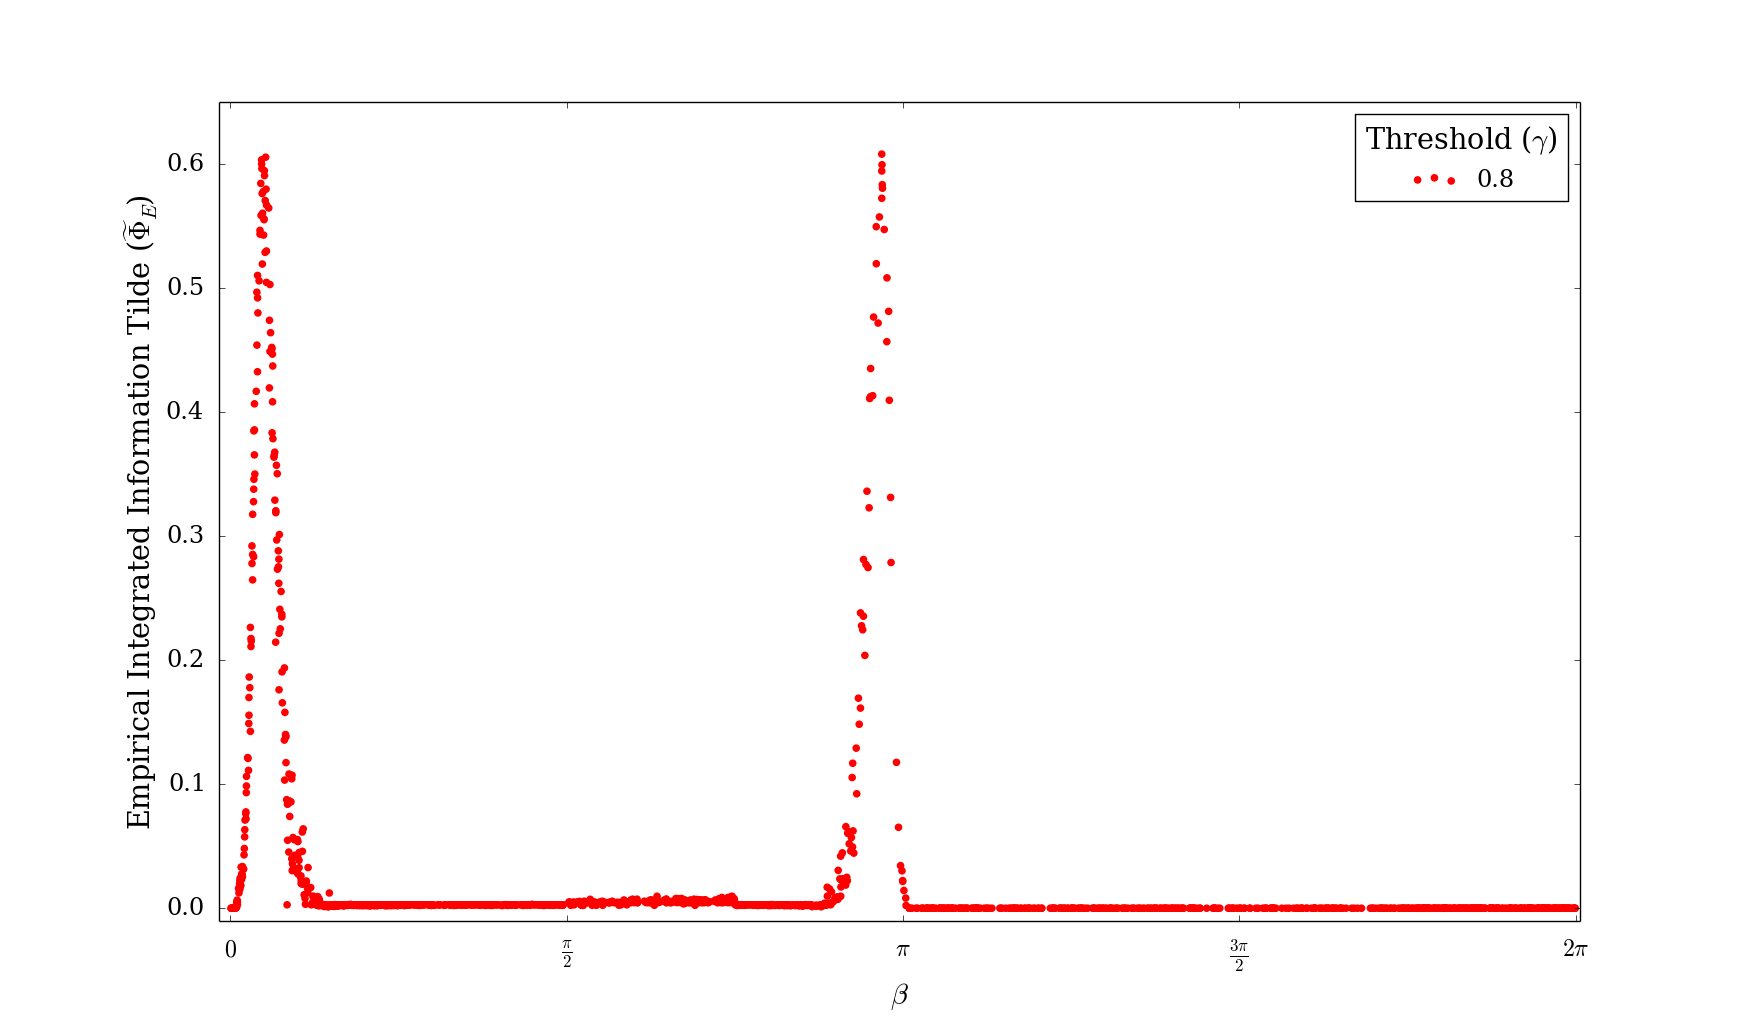
\includegraphics[scale = 0.2]{figures/phi_tilde_vs_beta_ext}
		\caption{
			$\widetilde{\Phi}_E$ vs $\beta$ for $0 \leq \beta \leq 2\pi$.
			\label{fig:phi-tilde-vs-beta-ext}
		}
		\end{center}
		\vspace{4ex}
	\end{minipage}
	\begin{minipage}[b]{0.5\linewidth}
		\begin{center}
		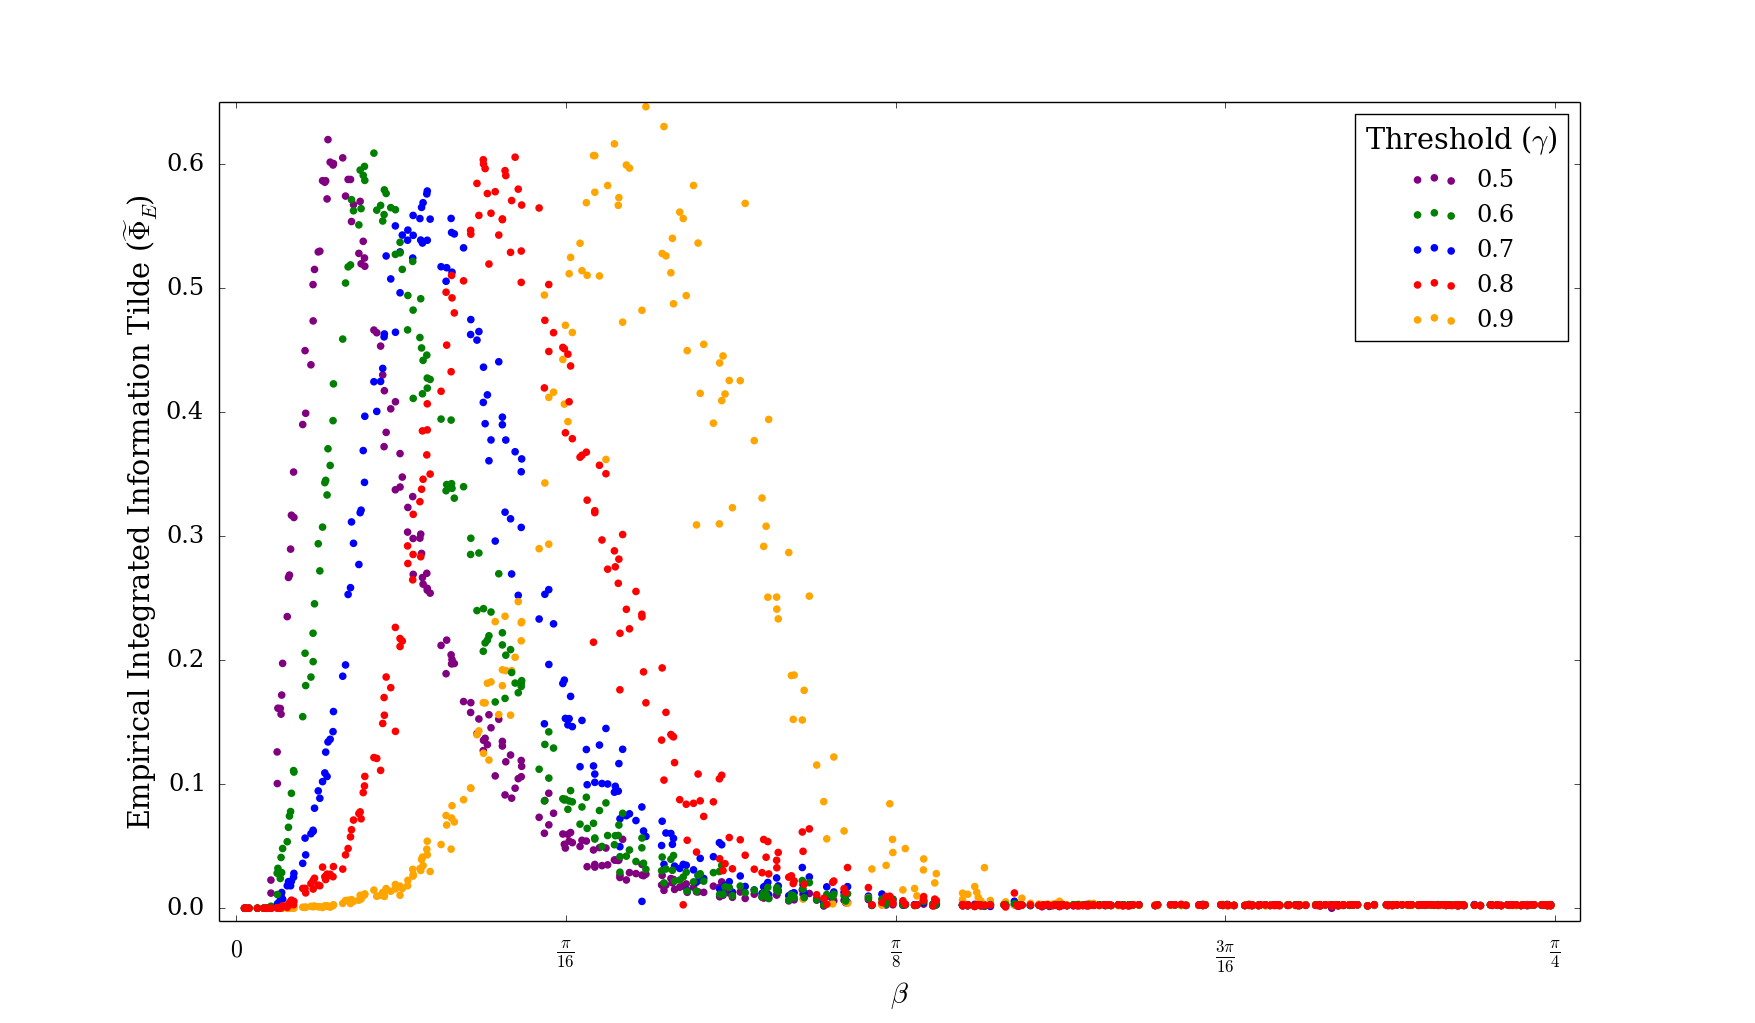
\includegraphics[scale = 0.2]{figures/phi_tilde_vs_beta_orig_multi}
		\caption{
			$\widetilde{\Phi}_E$ vs $\beta$ for $0 \leq \beta \leq \frac{\pi}{4}$\\ at multiple $\gamma$.
			\label{fig:phi-tilde-vs-beta-orig-multi}
		}
		\end{center}
		\vspace{4ex}
	\end{minipage}
	\begin{minipage}[b]{0.5\linewidth}
		\begin{center}
		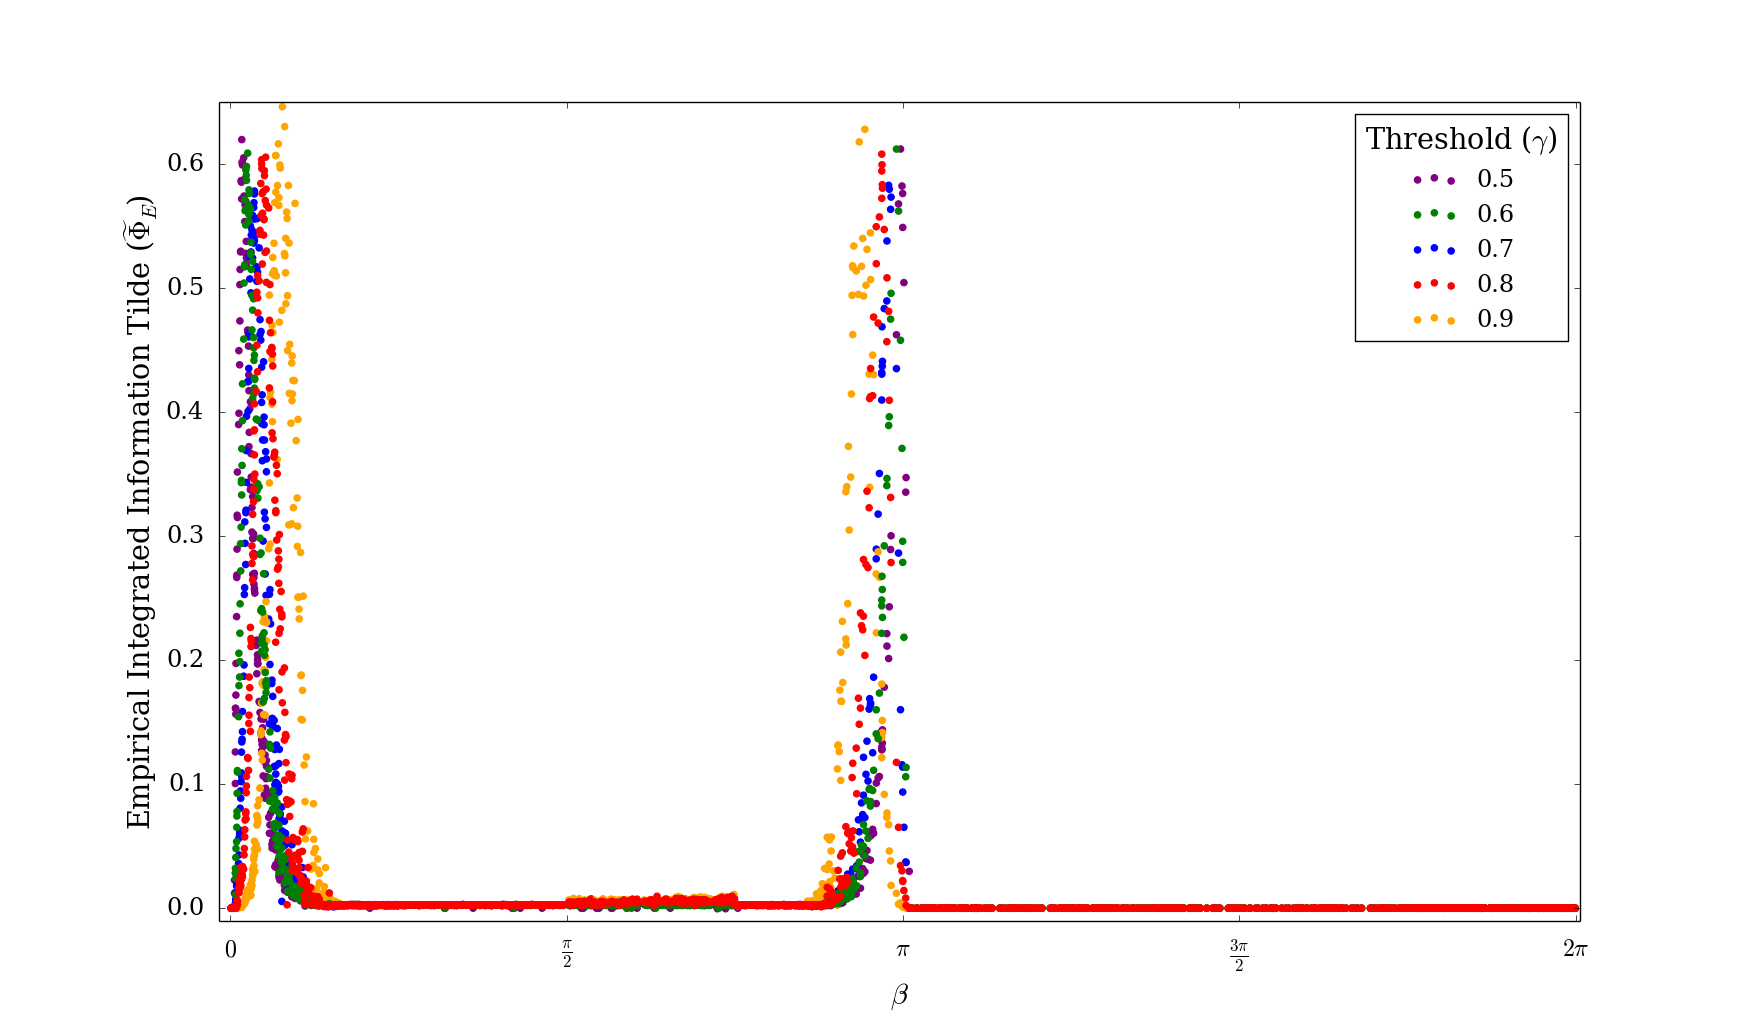
\includegraphics[scale = 0.2]{figures/phi_tilde_vs_beta_ext_multi}
		\caption{
			$\widetilde{\Phi}_E$ vs $\beta$ for $0 \leq \beta \leq 2\pi$\\ at multiple $\gamma$.
			\label{fig:phi-tilde-vs-beta-ext-multi}
		}
		\end{center}
		\vspace{4ex}
	\end{minipage}

\end{figure}

% ----------
% Phi vs Psi
% ----------
\subsubsection{Empirical Integrated Information ($\Phi_{E}$) vs Global Synchrony ($\Psi$)}
\label{sec:app:osc:res:phi-v-psi}

We also considered the relationship between our measures for integrated information and global synchrony ($\Psi$) for multiple thresholds ($\gamma$). For all values of $\gamma$ considered, we observed a parabolic peak with a maximum $\Psi$ ranging from $\Psi \approx 0.44$ to $\Psi \approx 0.81$ increasing with $\gamma$. As with $\Phi_{E}$ versus $\beta$, the value of $\Phi_E$ decreases from $\gamma = 0.5$ to $\gamma = 0.7$, but then increases from $\gamma = 0.7$ to $\gamma = 0.9$. This is depicted in Figure \ref{fig:phi-vs-psi-multi}. It is also worth noting that for $\gamma = 0.6$, $\gamma = 0.7$ and $\gamma = 0.8$, the value of $\Phi_E$ drops below zero before increasing. However, this dip is not symmetrical, as it does not reappear when $\Phi_E$ decreases on the right end of the peak. Finally, as $\gamma$ increases, it is possible to see a shift from a right skew towards a left skew, with $\gamma = 0.8$ showing the most symmetrical peak. 

\begin{figure}[H]
\begin{center}
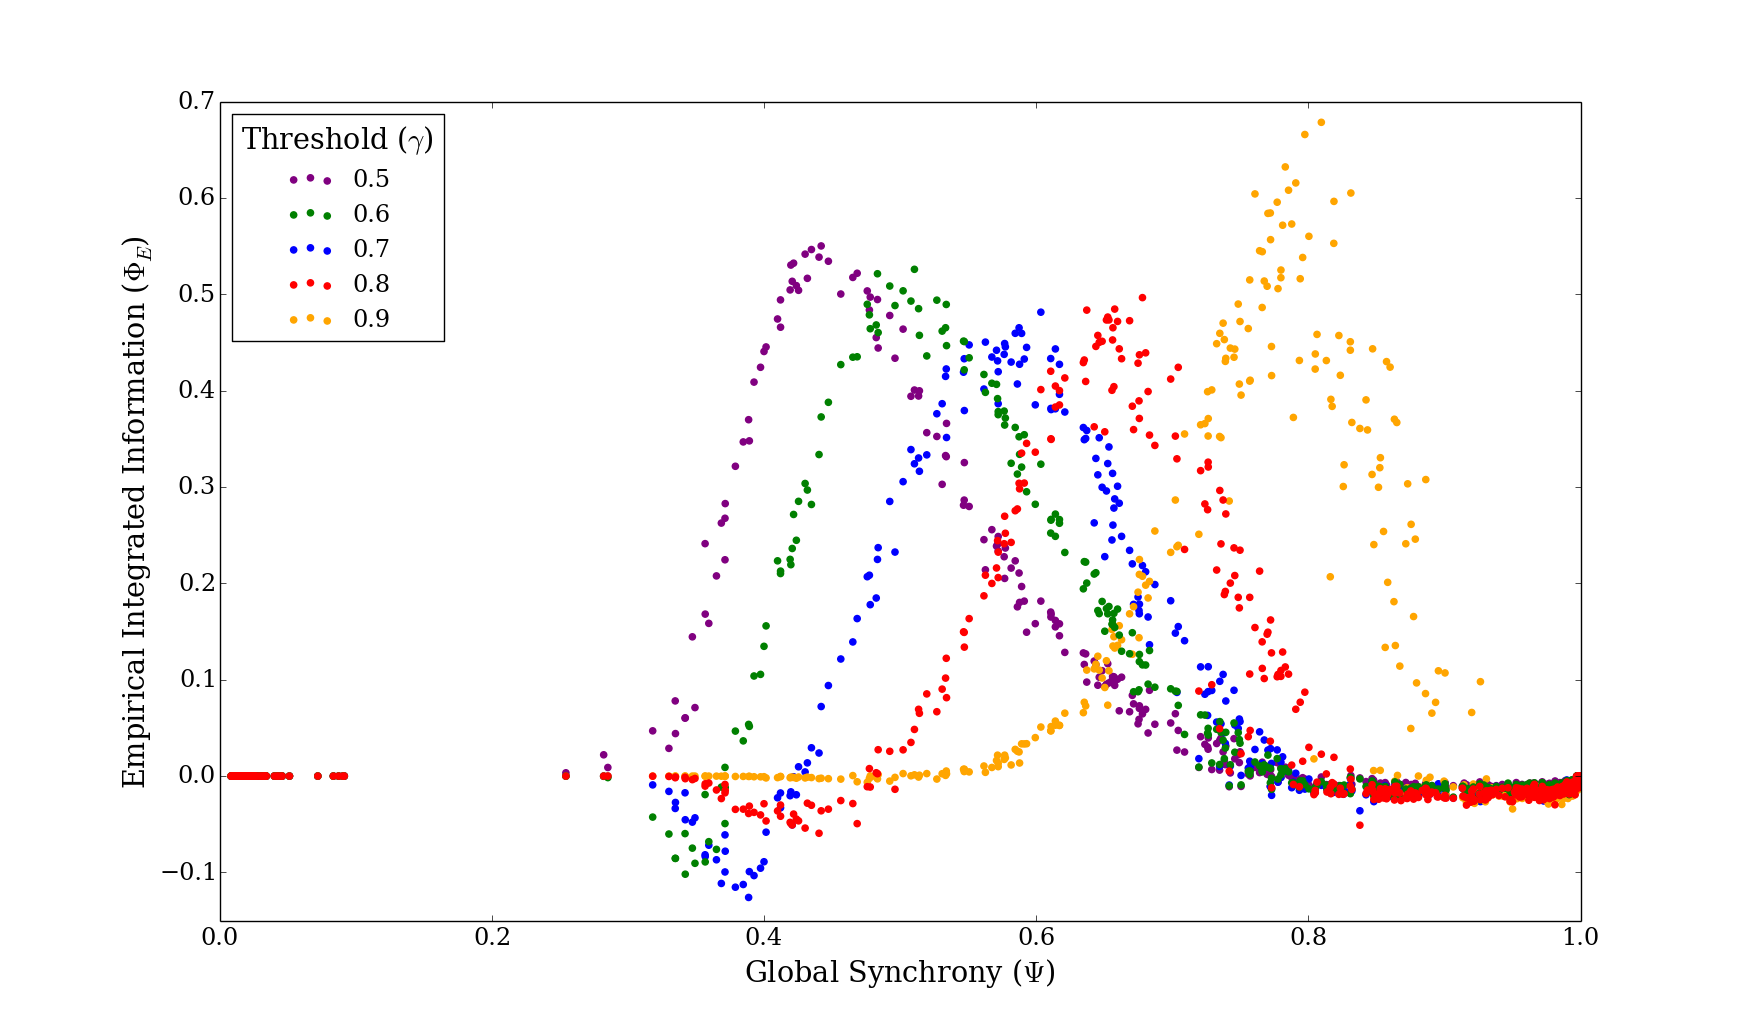
\includegraphics[scale = 0.35]{figures/phi_vs_psi_multi}
\caption{
	Empirical Integrated Information ($\Phi_E$) vs Global Synchrony ($\Psi$).
	\label{fig:phi-vs-psi-multi}
}
\end{center}
\end{figure}

% ----------------
% Phi Tilde vs Psi
% ----------------
\subsubsection{Empirical Integrated Information Tilde ($\widetilde{\Phi}_{E}$) vs Global Synchrony ($\Psi$)}
\label{sec:app:osc:res:phi-tilde-v-psi}

As can be seen in Figure \ref{fig:phi-tilde-vs-psi-multi}, the relationship between $\widetilde{\Phi}_{E}$ and $\Psi$ is comparable to the one between $\Phi_E$ and $\Psi$ as described in Section \ref{sec:app:osc:res:phi-v-psi}. The key difference is that since $\widetilde{\Phi}_{E}$ cannot take negative values, there is no dip in $\widetilde{\Phi}_{E}$ preceding the occurrence of the peak for any threshold.

\begin{figure}[H]
\begin{center}
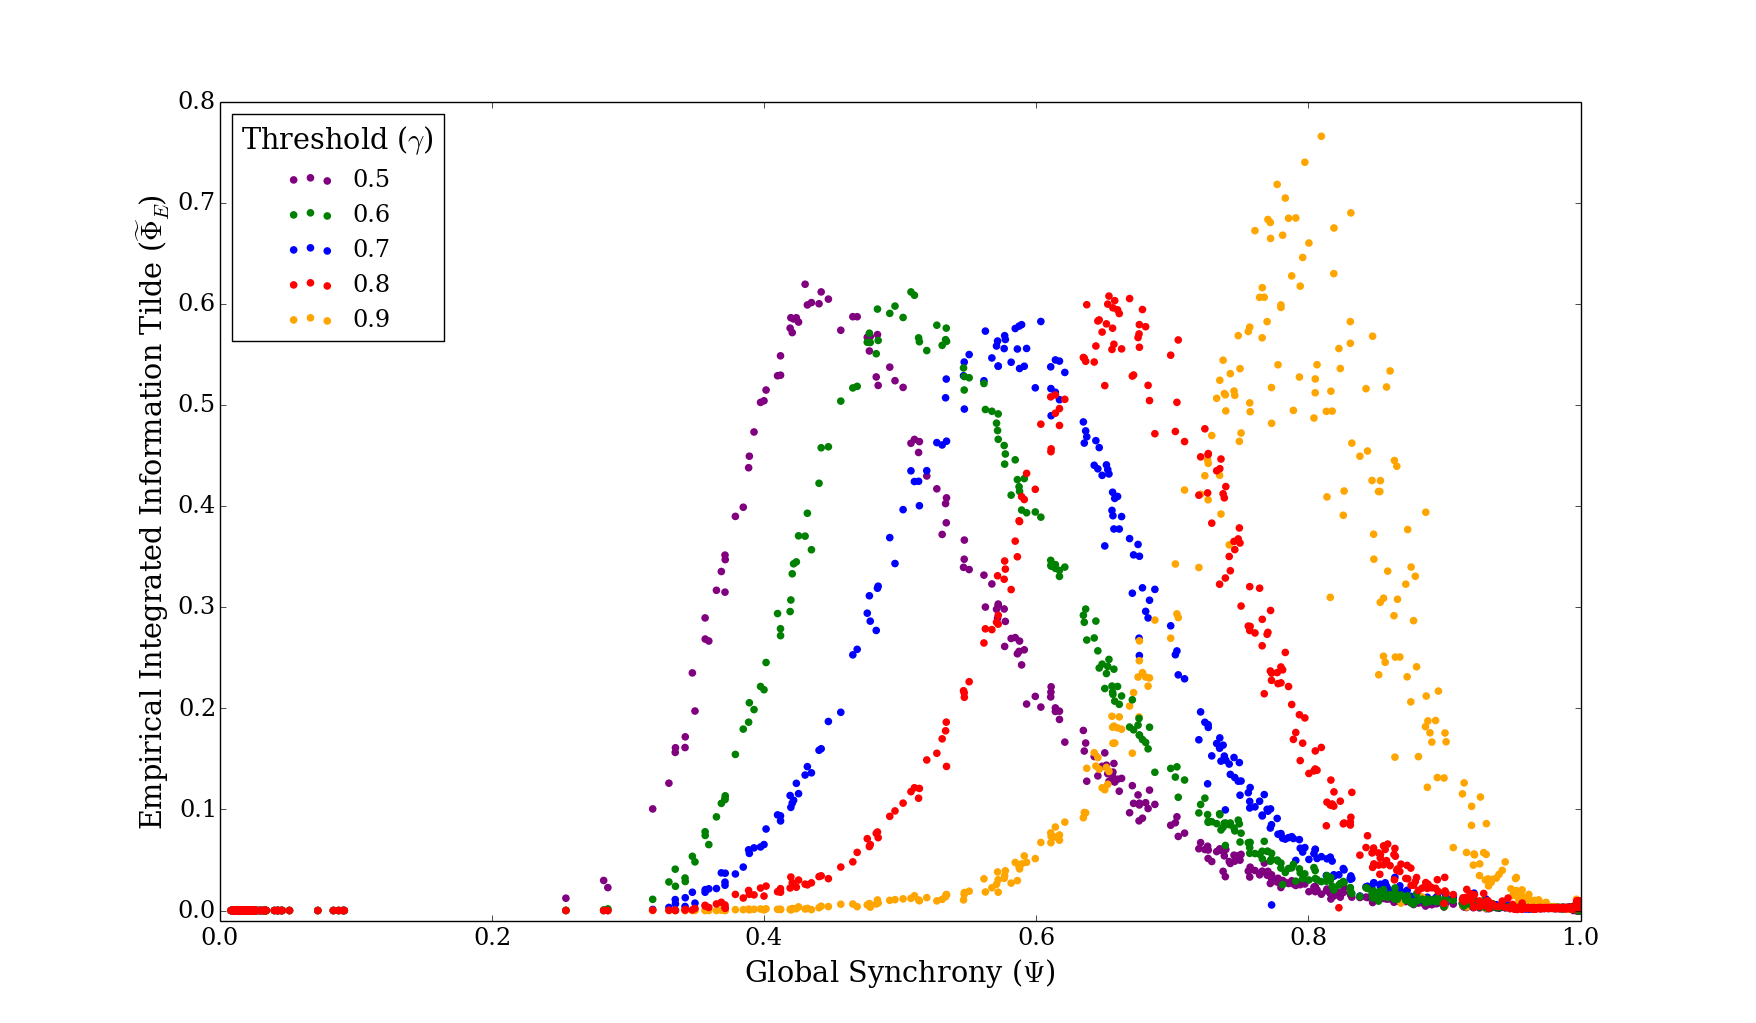
\includegraphics[scale = 0.35]{figures/phi_tilde_vs_psi_multi}
\caption{
	Empirical Integrated Information Tilde ($\widetilde{\Phi}_E$) vs Global Synchrony ($\Psi$).
	\label{fig:phi-tilde-vs-psi-multi}
}
\end{center}
\end{figure}

% --------------------------
% Phi vs Metastability Index
% --------------------------
\subsubsection{Empirical Integrated Information ($\Phi_{E}$) vs Metastability Index ($\lambda$)}
\label{sec:app:osc:res:phi-v-lambda}

An important relationship that we were looking to examine was the correlation between our measures of integrated information and measures that indicated the level of metastability exhibited by a given system. We first considered $\Phi_{E}$ and Shanahan's metastability index $\lambda$, as defined in Section \ref{sec:bg:lambda}.

\begin{figure}[H]
\begin{center}
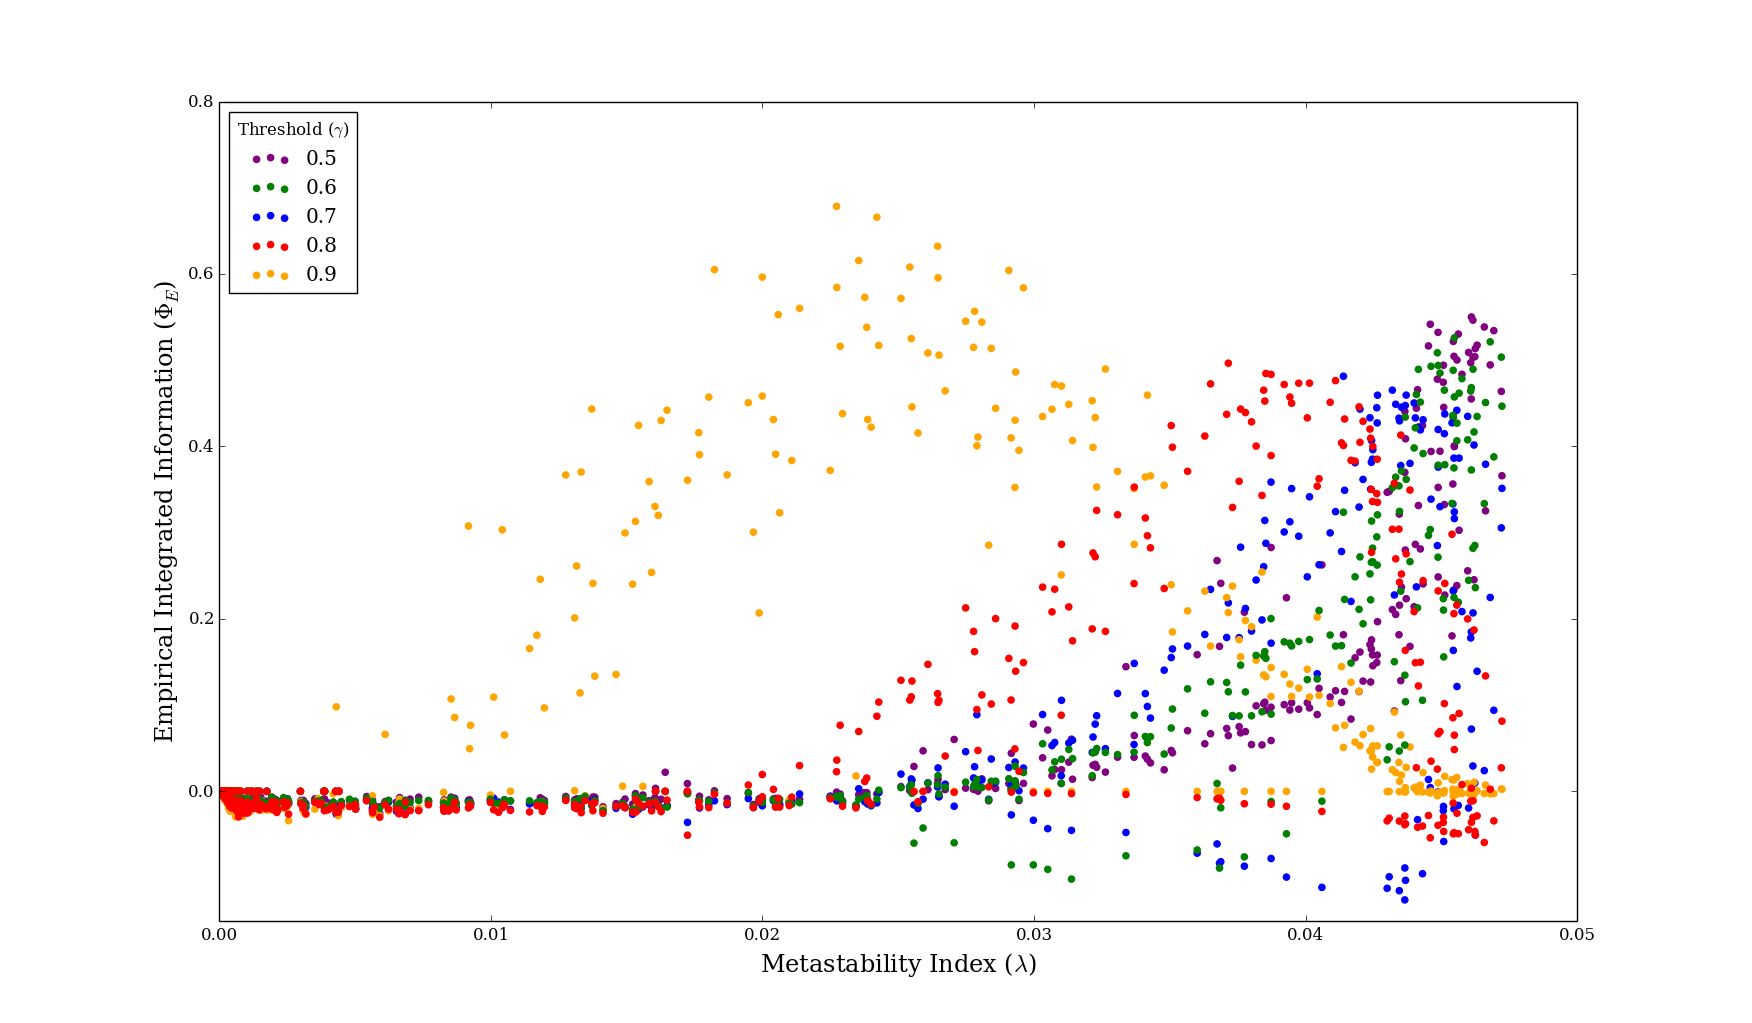
\includegraphics[scale = 0.35]{figures/phi_vs_lambda_multi}
\caption{
	Empirical Integrated Information ($\Phi_E$) vs Metastability Index ($\lambda$).
	\label{fig:phi-vs-lambda-multi}
}
\end{center}
\end{figure}

Initially we plotted the results for all of our values of $\gamma$, as shown in Figure \ref{fig:phi-vs-lambda-multi}. We noticed that the for the highest threshold, $\gamma = 0.9$, the shape of the plot was considerably different than for the rest of the thresholds. Instead of a peak between $\lambda \approx 0.037$ and $\lambda \approx 0.046$, with a  heavy left skew, the peak for $\gamma = 0.9$ was relatively symmetrical, centred around $\lambda \approx 0.023$. At the other end of the spectrum, when $\gamma = 0.5$, the plot did not show a complete peak, but rather a exponential-like curve. These plots are shown in Figures \ref{fig:phi_vs_lambda_5} and \ref{fig:phi_vs_lambda_9}.

\begin{figure}[H] 
	\label{fig:phi-vs-lambda-extremes} 
	\begin{minipage}[b]{0.5\linewidth}
		\begin{center}
		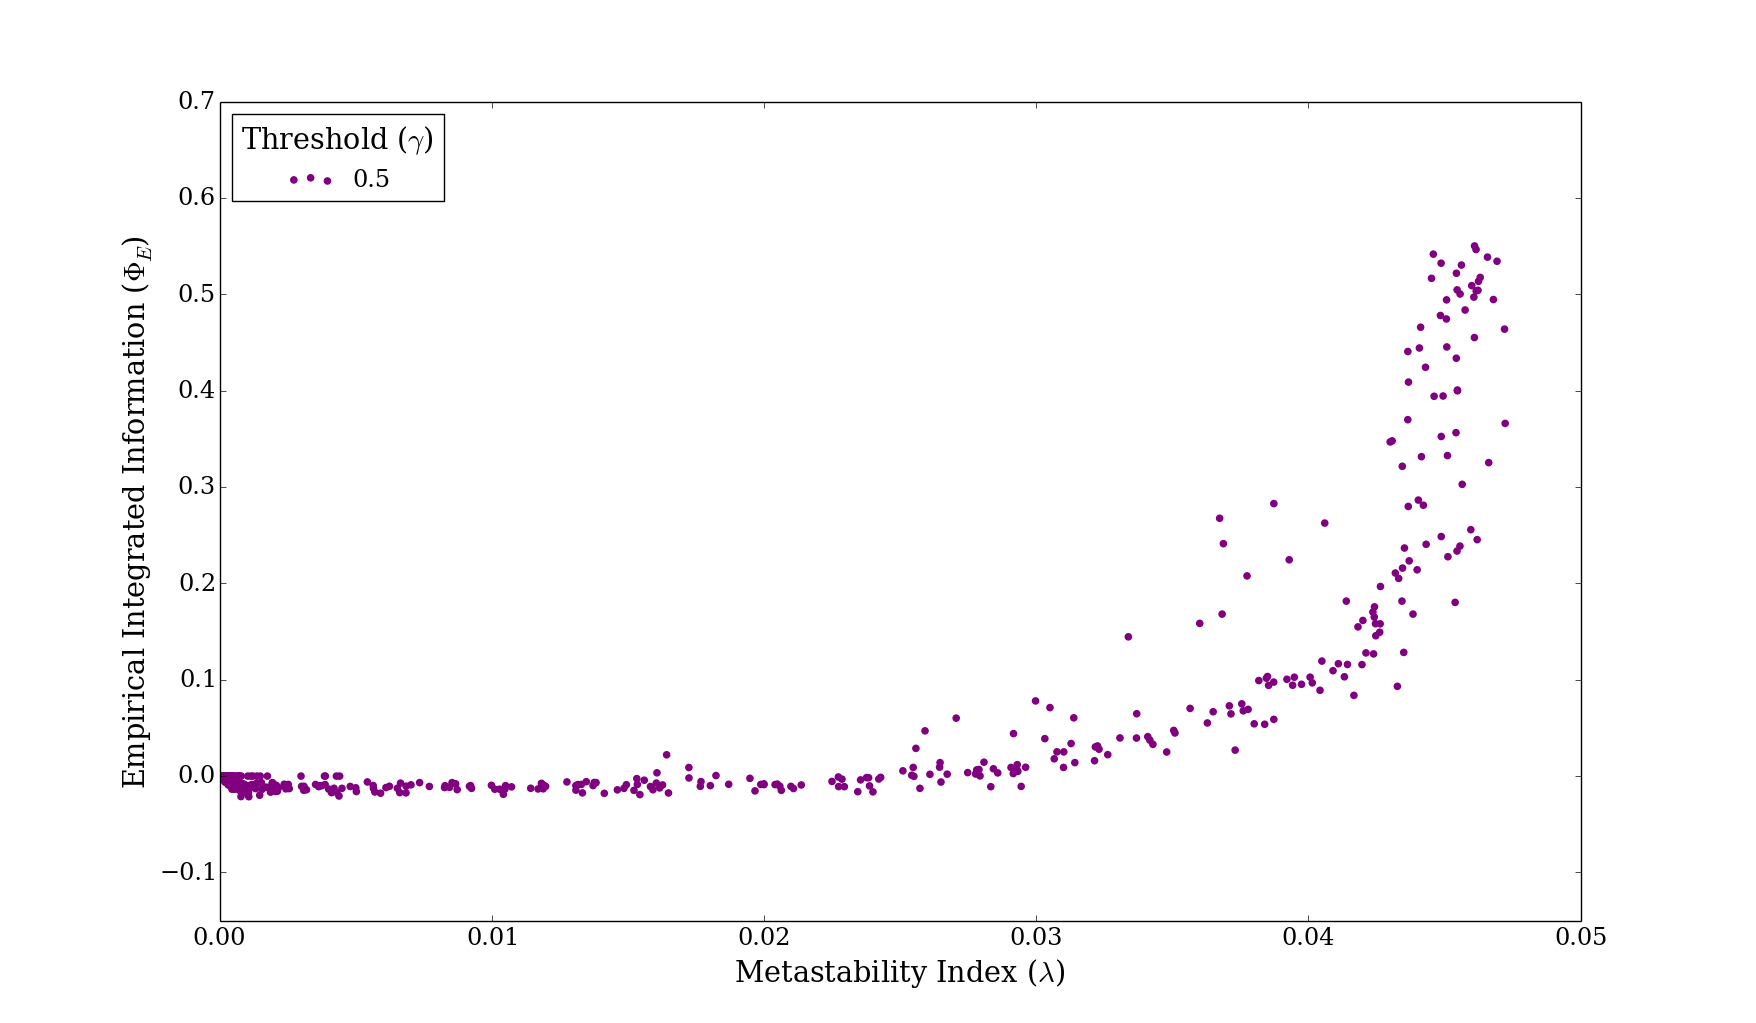
\includegraphics[scale = 0.2]{figures/phi_vs_lambda_5}
		\caption{
			$\Phi_E$ vs $\lambda$ at $\gamma = 0.5$.
			\label{fig:phi_vs_lambda_5}
		}
		\end{center}
		\vspace{2ex}
	\end{minipage}
	\begin{minipage}[b]{0.5\linewidth}
		\begin{center}
		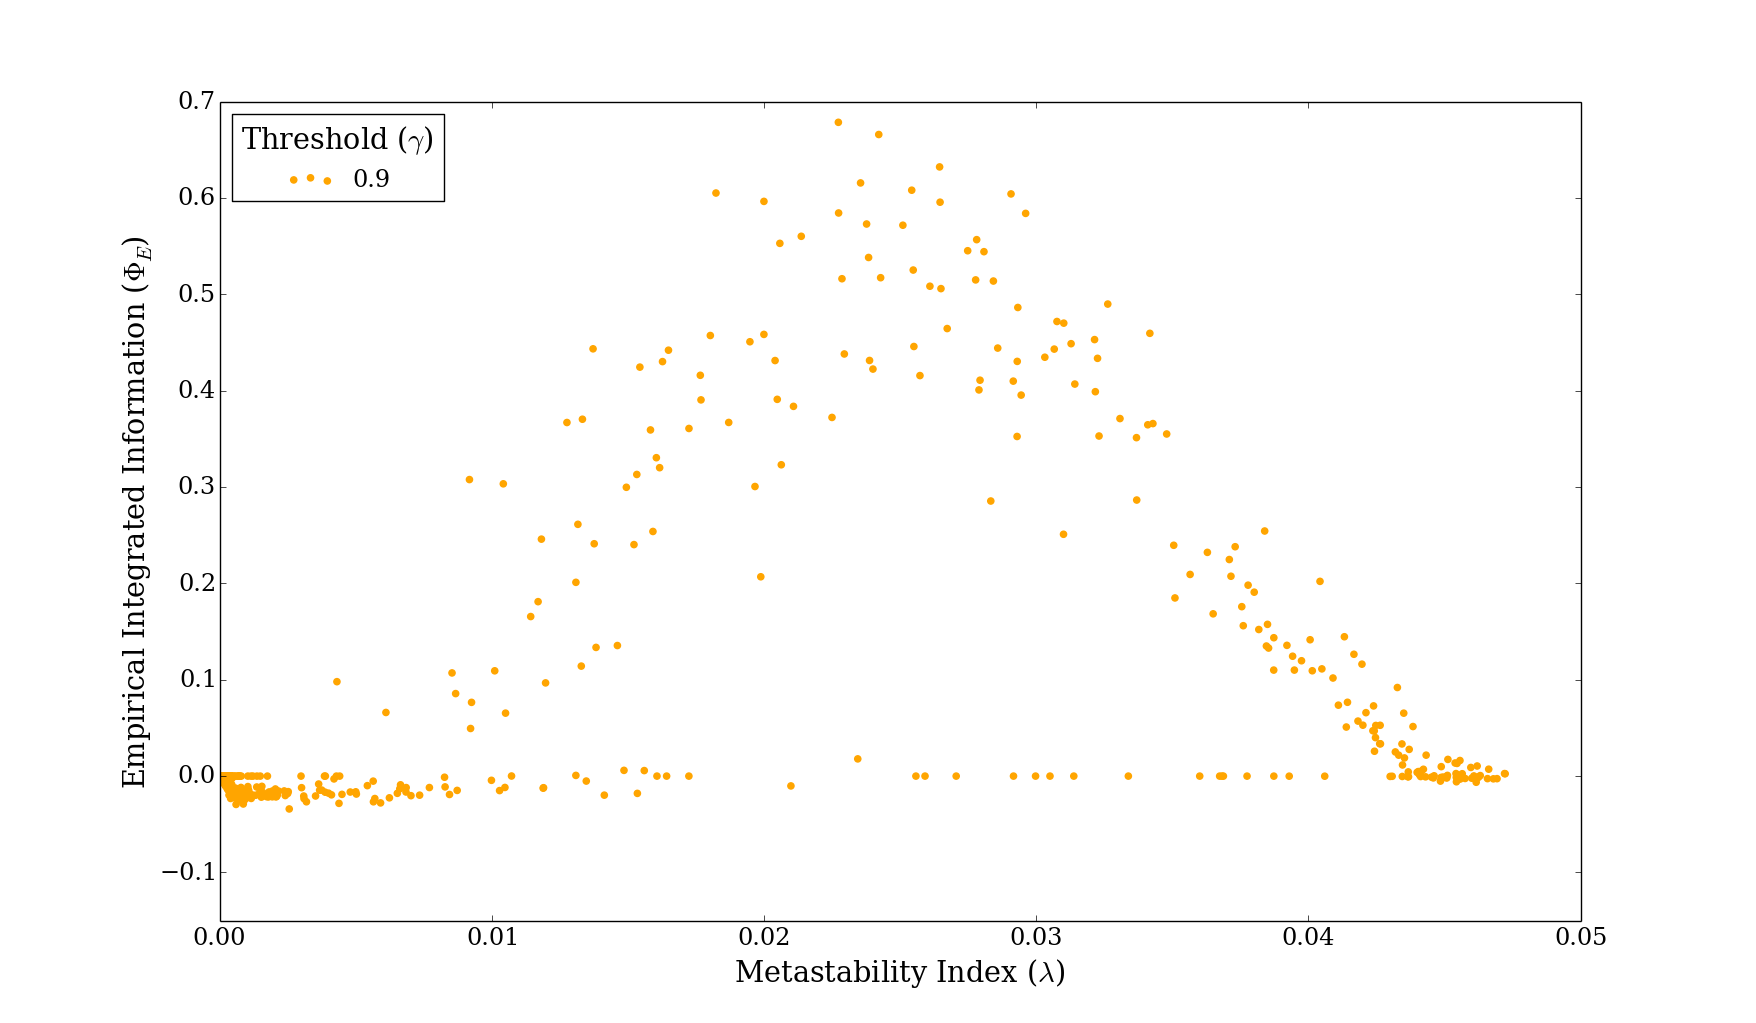
\includegraphics[scale = 0.2]{figures/phi_vs_lambda_9}
		\caption{
			$\Phi_E$ vs $\lambda$ at $\gamma = 0.9$.
			\label{fig:phi_vs_lambda_9}
		}
		\end{center}
		\vspace{2ex}
	\end{minipage}
\end{figure}

We then considered thresholds 0.6, 0.7 and 0.8 to better examine the relationship between these two measures without accounting for the \textit{extreme} values of $\gamma$. We observe a heavily left skewed peak that shifts left as the threshold increases, reaching a maximum of $\Phi_E \approx 0.5$. It is also important to note that there is a considerable amount of noise in the range of $0.025 < \lambda < 0.045$. In this region, values for $\lambda$ that produce relatively high values of $\Phi$ also lead to negative values.

\begin{figure}[H]
\begin{center}
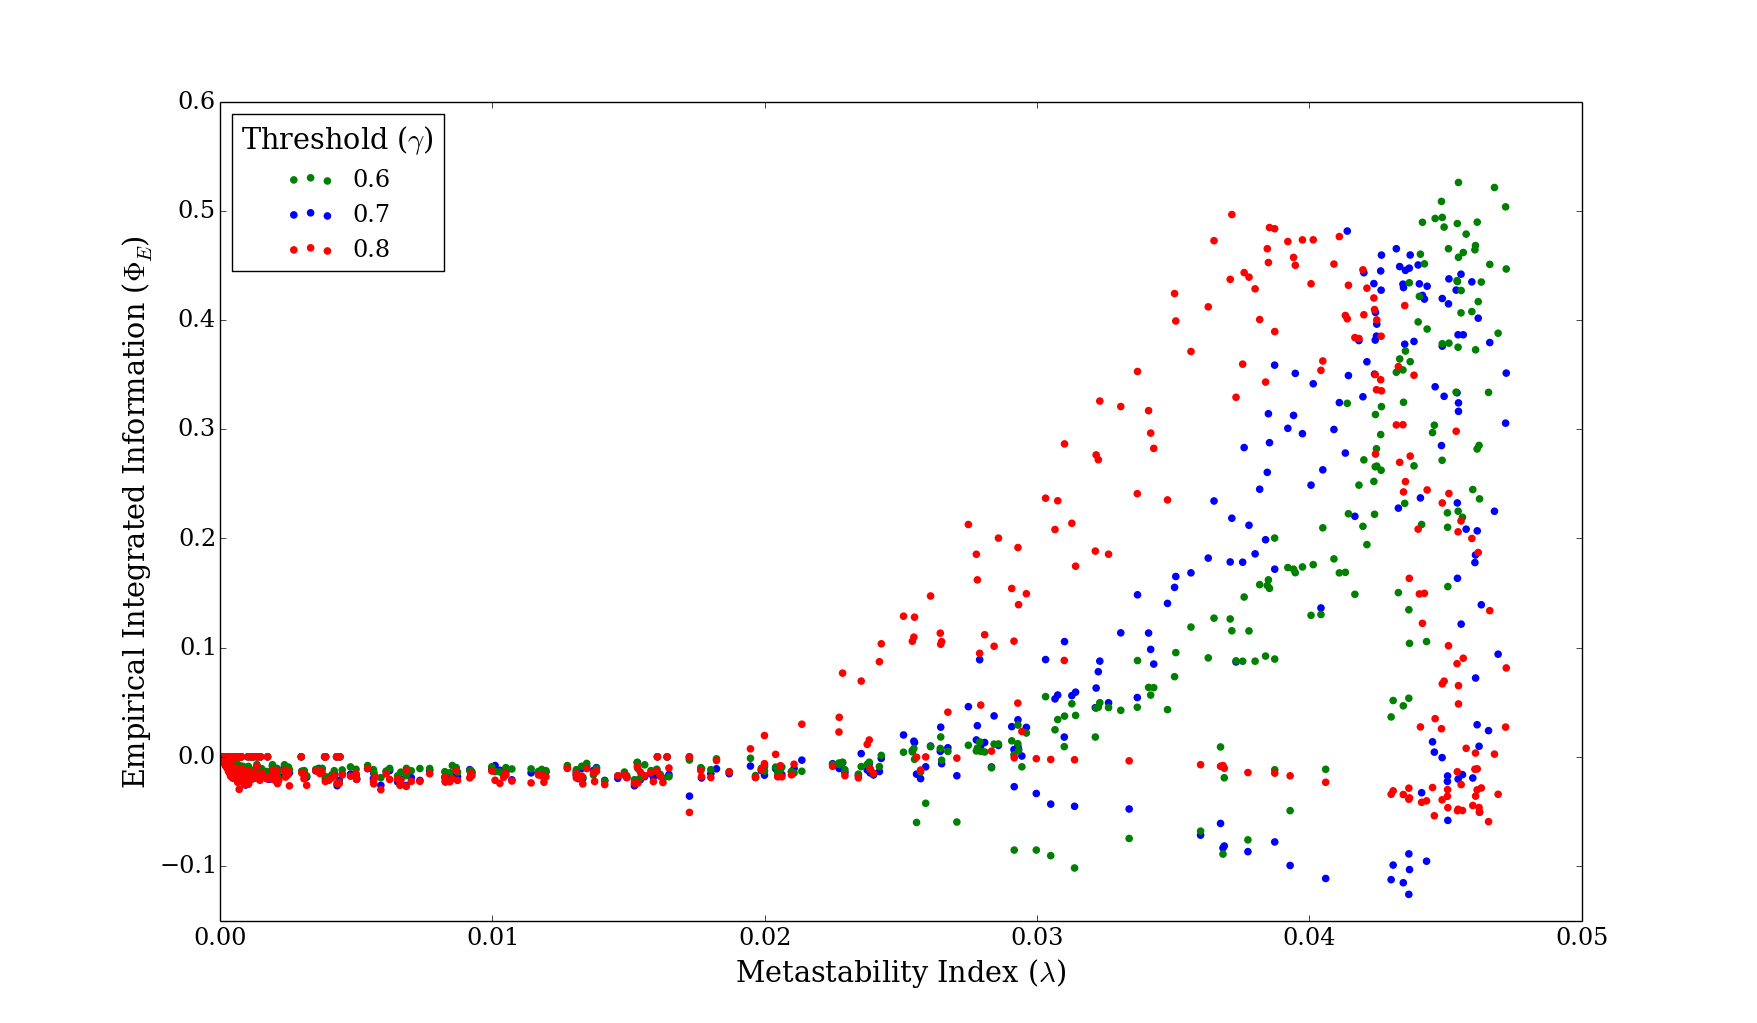
\includegraphics[scale = 0.35]{figures/phi_vs_lambda_mid}
\caption{
	Empirical Integrated Information ($\Phi_E$) vs Metastability Index ($\lambda$) at mid-range synchronisation thresholds ($\gamma$).
	\label{fig:phi-vs-lambda-mid}
}
\end{center}
\end{figure}

% --------------------------------
% Phi Tilde vs Metastability Index
% --------------------------------
\subsubsection{Empirical Integrated Information Tilde ($\widetilde{\Phi}_{E}$) vs Metastability Index ($\lambda$)}
\label{sec:app:osc:res:phi-tilde-v-lambda}

We proceeded to extend our analysis between integrated information and Shanahan's metastability index to our implementation of $\widetilde{\Phi}_{E}$. We found the same discrepancies at \textit{extreme} thresholds described in Section \ref{sec:app:osc:res:phi-v-lambda} so we focused on plotting the correlation given $\gamma$ values of 0.6, 0.7 and 0.8. We can see in Figure \ref{fig:phi-tilde-vs-lambda-mid} that the correlation is comparable to the one using $\Phi_E$, with slightly less noise occurring in the range $0.025 < \lambda < 0.045$ and specifically for $\gamma = 0.6$

\begin{figure}[H]
\begin{center}
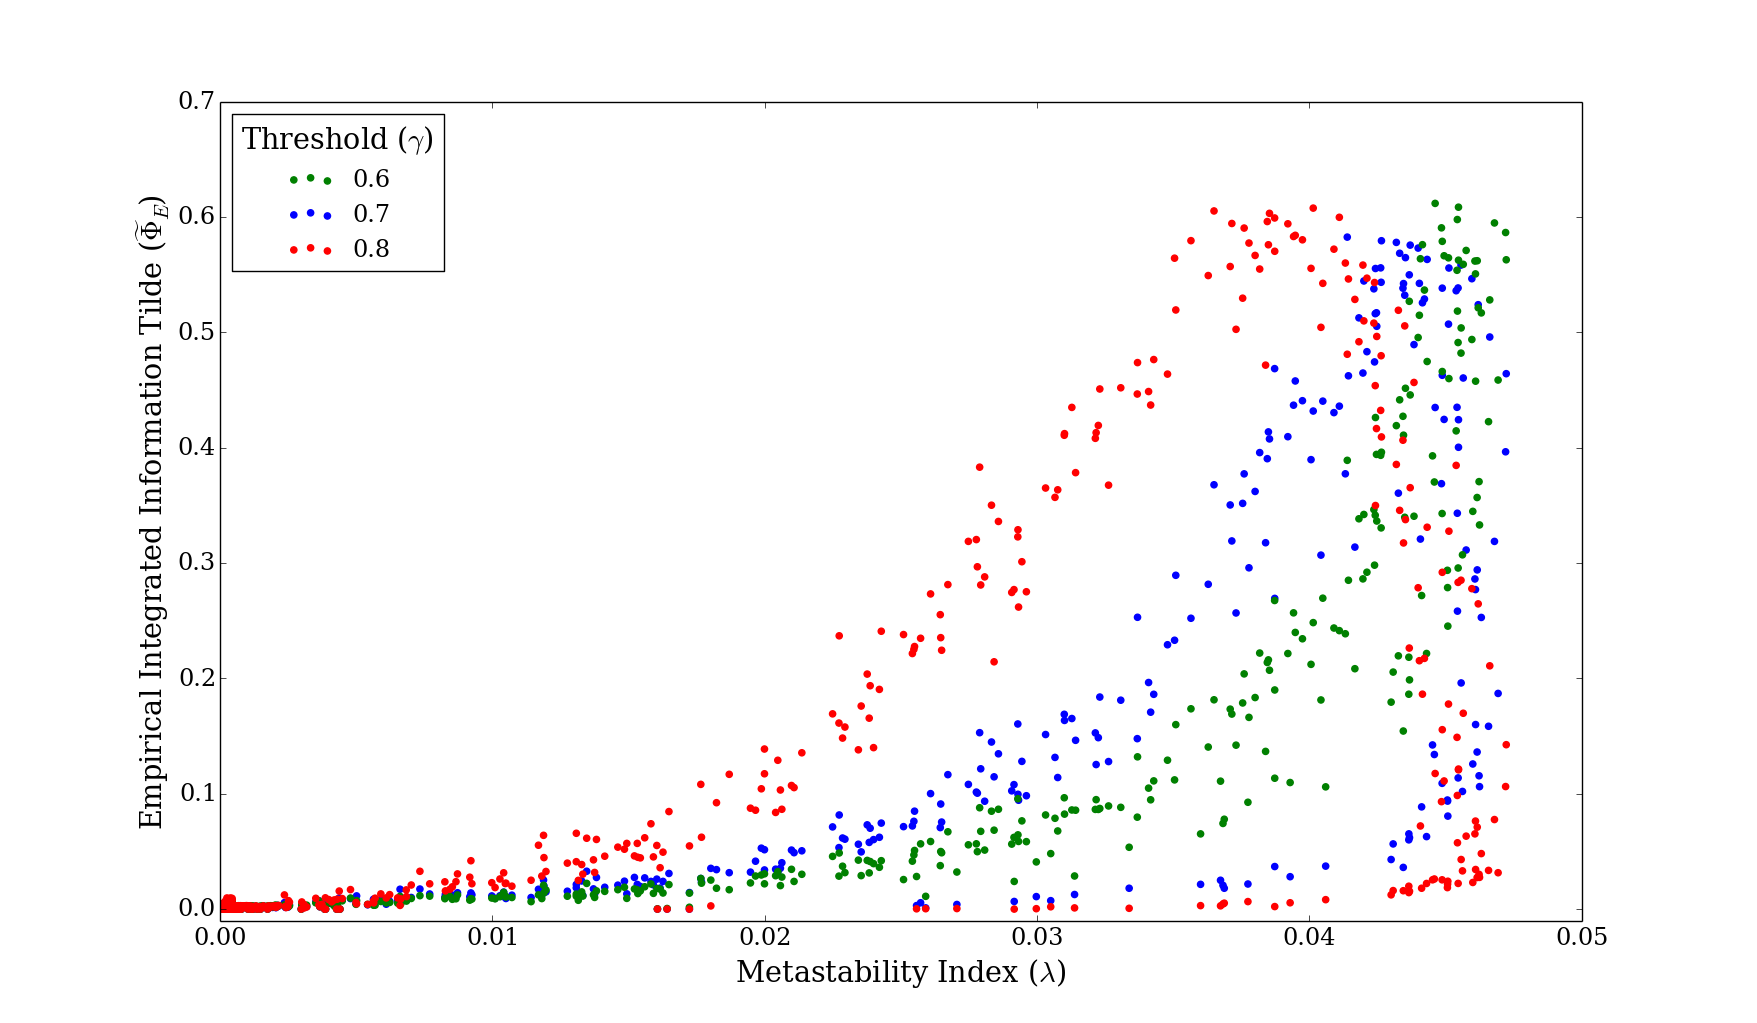
\includegraphics[scale = 0.35]{figures/phi_tilde_vs_lambda_mid}
\caption{
	Empirical Integrated Information Tilde ($\widetilde{\Phi}_E$) vs Metastability Index ($\lambda$) at mid-range synchronisation thresholds ($\gamma$).
	\label{fig:phi-tilde-vs-lambda-mid}
}
\end{center}
\end{figure}

% --------------------
% Phi vs Chimera Index
% --------------------
\subsubsection{Empirical Integrated Information ($\Phi_{E}$) vs Chimera Index ($\chi$)}
\label{sec:app:osc:res:phi-v-chi}

A second measure related to the metastability of a system is Shanahan's chimera index as defined in Section \ref{sec:bg:chi}. We considered the relationship between $\chi$ and $\Phi_{E}$ and confirmed a nearly identical behaviour as that between $\Phi_E$ and $\lambda$. These findings are consistent with the close relationship between $\chi$ and $\lambda$ presented in \cite{Shanahan2010} and in our results in Sections \label{sec:app:osc:res:meta-v-beta} and \label{sec:app:osc:res:chi-v-beta}.

\begin{figure}[H]
\begin{center}
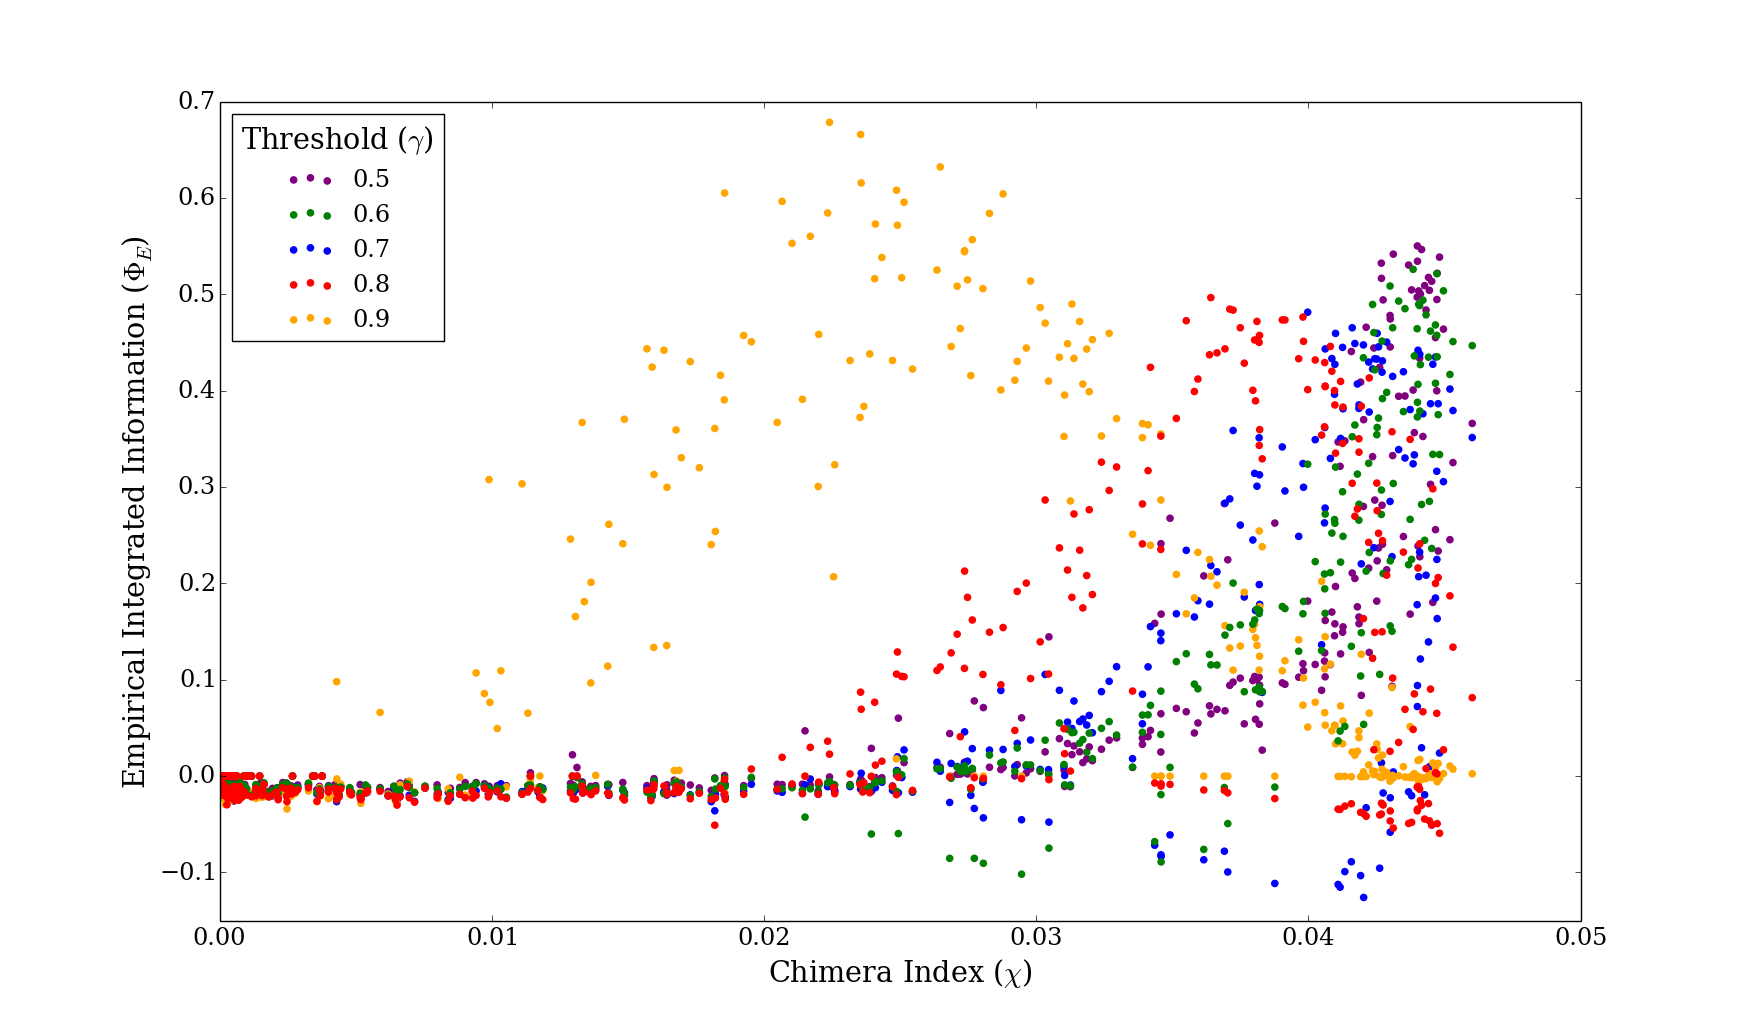
\includegraphics[scale = 0.35]{figures/phi_vs_chi_multi}
\caption{
	Empirical Integrated Information ($\Phi_E$) vs Chimera Index ($\chi$).
	\label{fig:phi-vs-chi-multi}
}
\end{center}
\end{figure}

Once more, we first created a plot for results encompassing all of the values of $\gamma$ used in our simulations, as shown in Figure \ref{fig:phi-vs-chi-multi}. As with $\lambda$ the \textit{extreme} values of $\gamma = 0.5$ and $\gamma = 0.9$ were not particularly in line with the rest of the values of $\gamma$. These plots are shown in Figures \ref{fig:phi_vs_chi_5} and \ref{fig:phi_vs_chi_9}.

\begin{figure}[H] 
	\label{fig:phi-vs-chi-extremes} 
	\begin{minipage}[b]{0.5\linewidth}
		\begin{center}
		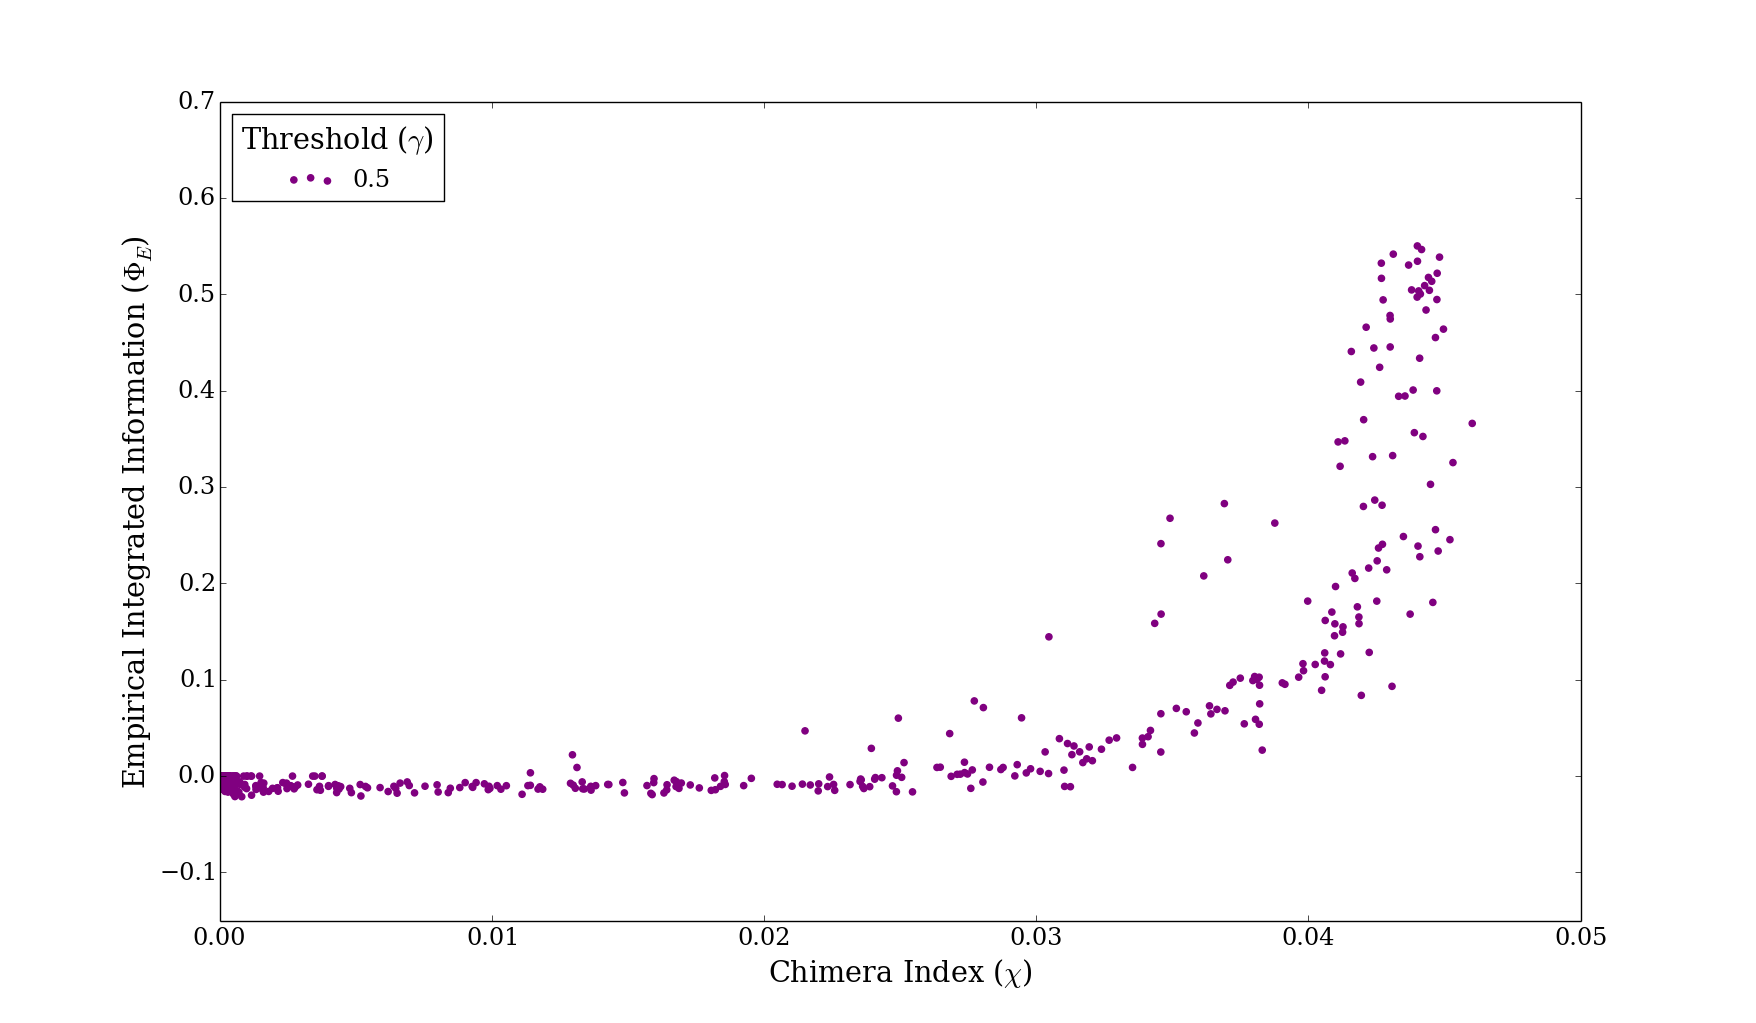
\includegraphics[scale = 0.2]{figures/phi_vs_chi_5}
		\caption{
			$\Phi_E$ vs $\lambda$ at $\gamma = 0.5$.
			\label{fig:phi_vs_chi_5}
		}
		\end{center}
		\vspace{2ex}
	\end{minipage}
	\begin{minipage}[b]{0.5\linewidth}
		\begin{center}
		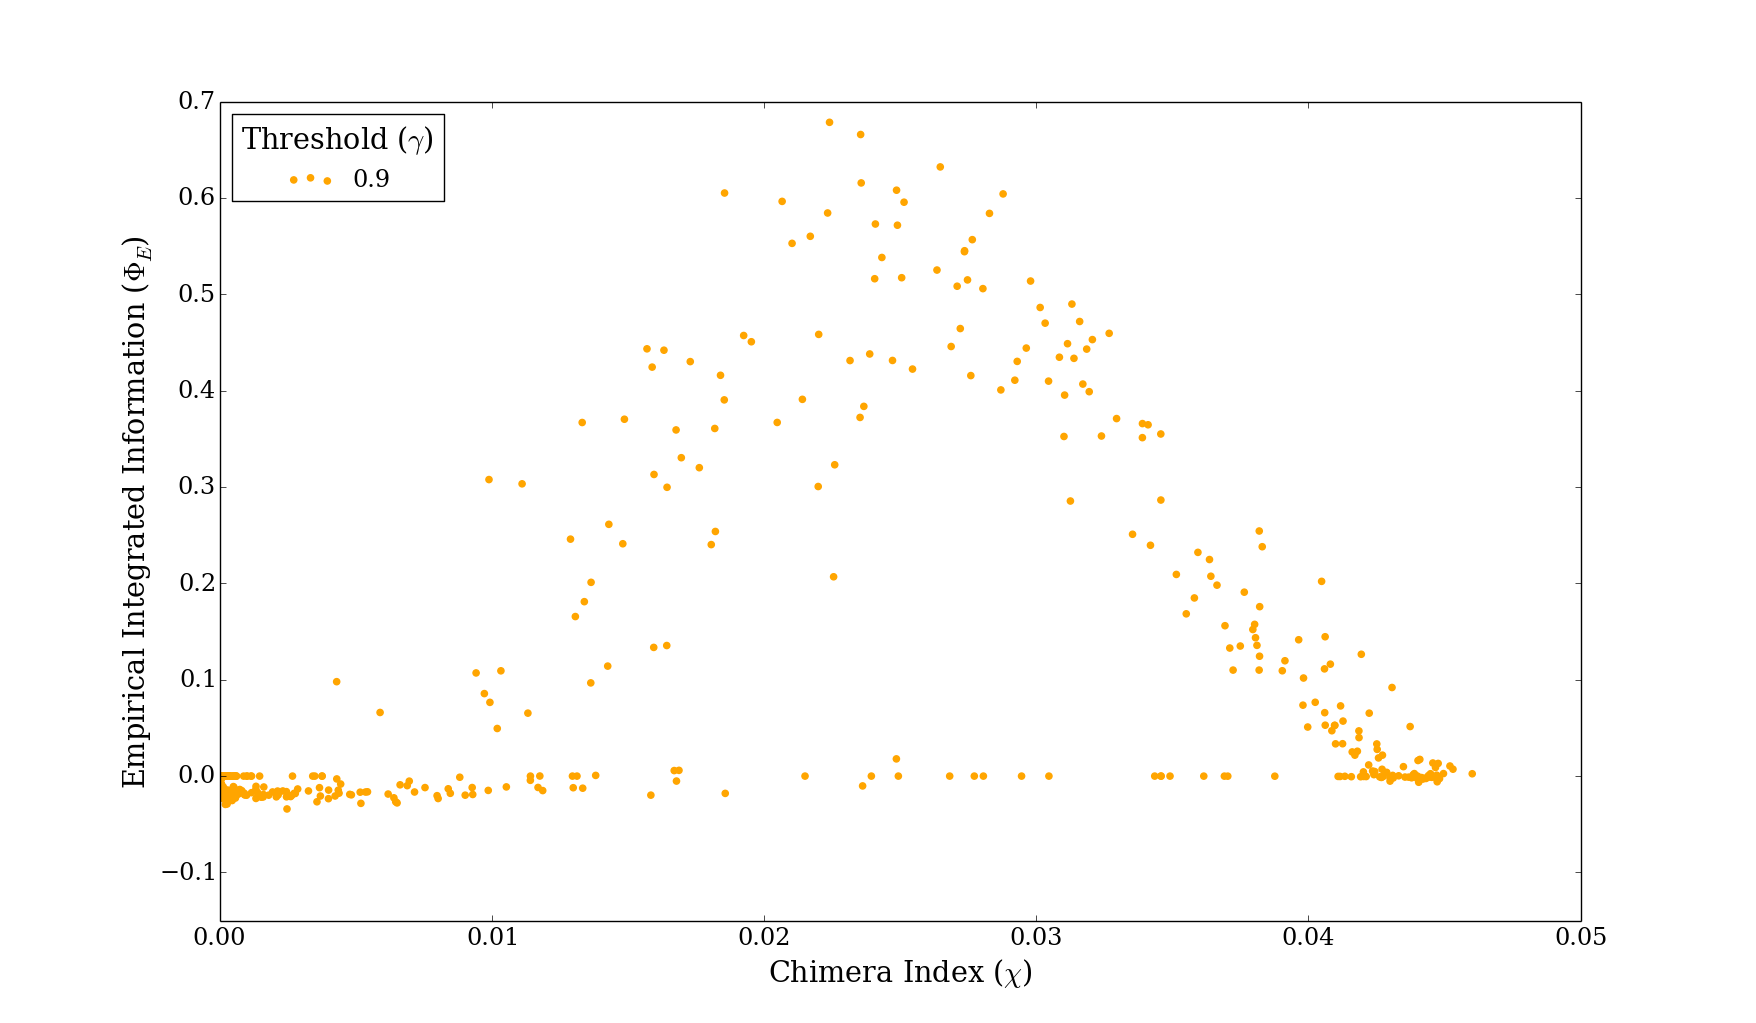
\includegraphics[scale = 0.2]{figures/phi_vs_chi_9}
		\caption{
			$\Phi_E$ vs $\lambda$ at $\gamma = 0.9$.
			\label{fig:phi_vs_chi_9}
		}
		\end{center}
		\vspace{2ex}
	\end{minipage}
\end{figure}

We thus plotted thresholds 0.6, 0.7 and 0.8 separately, obtaining the same results as in Section \ref{sec:app:osc:res:phi-v-lambda}. Once more, the plots showed a heavily left skewed peak, shifting towards the left as $\gamma$ increases and reaching a maximum of $\Phi_E \approx 0.5$. The noise in the range of $0.025 < \lambda 0.045$ was also present, with $\chi$ values producing both relatively high $\Phi$ as well as negative values.

\begin{figure}[H]
\begin{center}
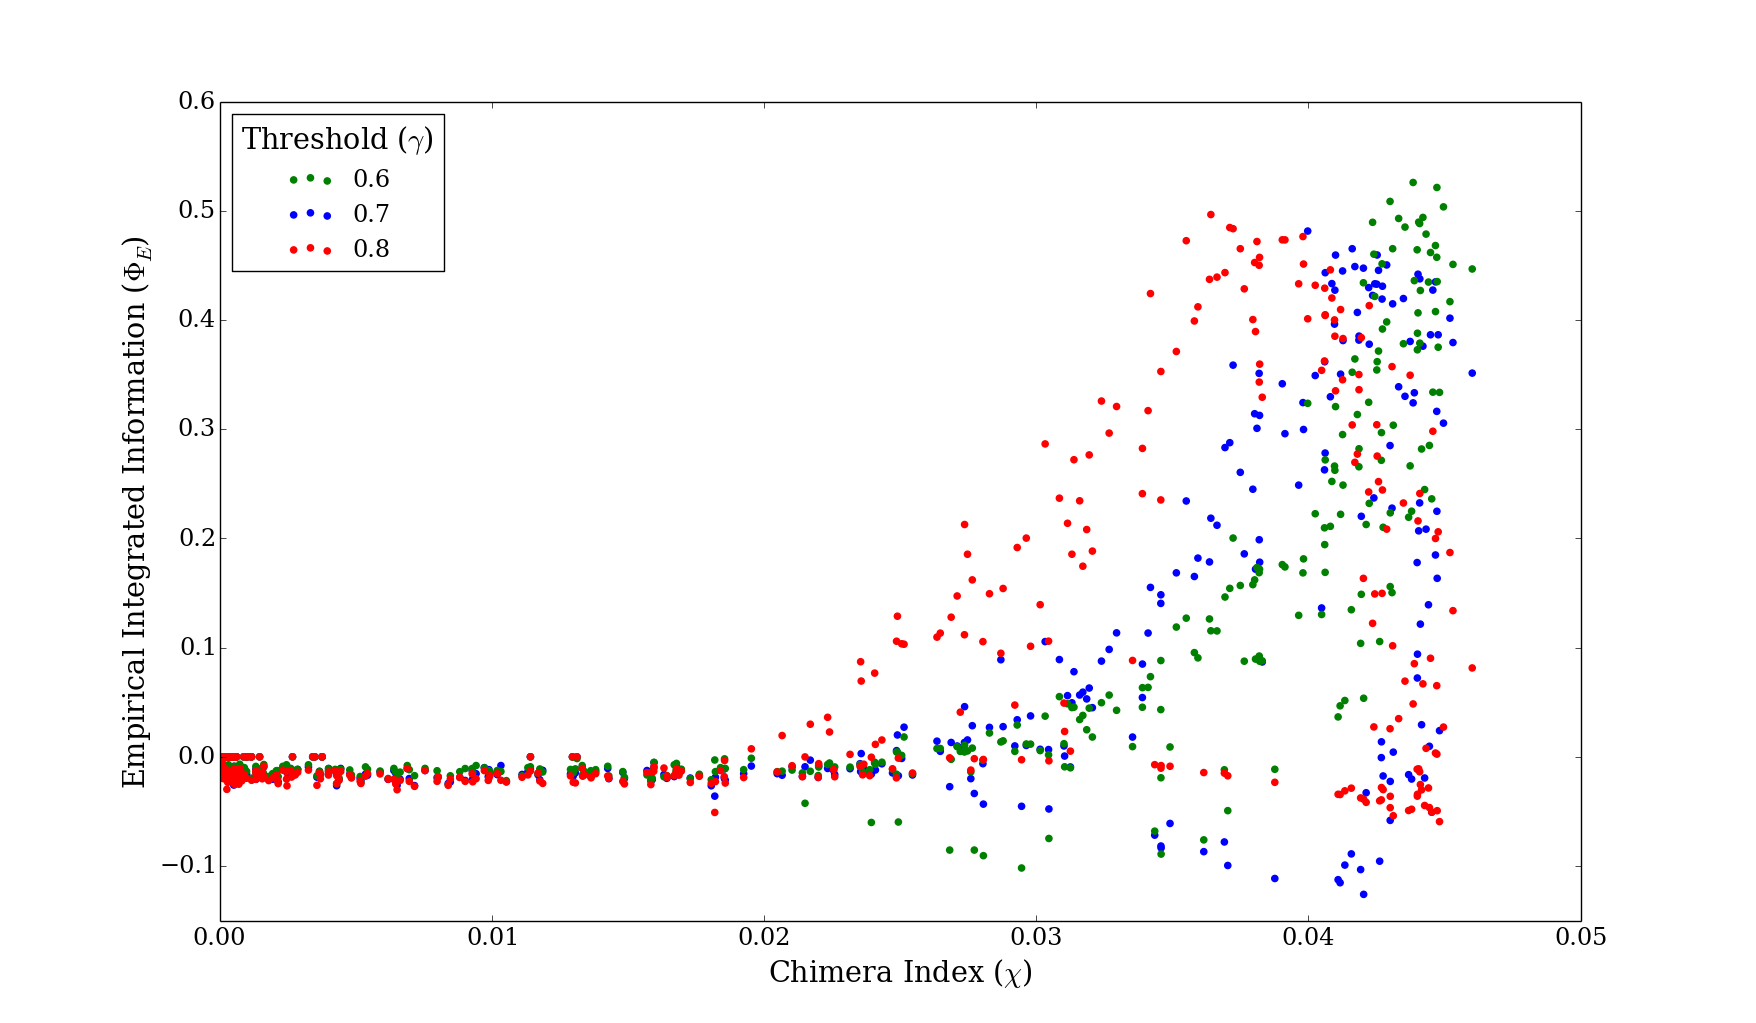
\includegraphics[scale = 0.35]{figures/phi_vs_chi_mid}
\caption{
	Empirical Integrated Information ($\Phi_E$) vs Chimera Index ($\chi$) at mid-range synchronisation thresholds ($\gamma$).
	\label{fig:phi-vs-chi-mid}
}
\end{center}
\end{figure}

% --------------------------
% Phi Tilde vs Chimera Index
% --------------------------
\subsubsection{Empirical Integrated Information Tilde ($\widetilde{\Phi}_{E}$) vs Chimera Index ($\chi$)}
\label{sec:app:osc:res:phi-tilde-v-chi}

As with all our analyses involving integrated information, we then plotted the same relationship, but using our implementation of $\widetilde{\Phi}_{E}$. The same discrepancies at \textit{extreme} thresholds reappeared and so we once more plotted the correlation for $\gamma$ values of 0.6, 0.7 and 0.8 only. Figure \ref{fig:phi-tilde-vs-lambda-mid} shows that the correlation closely resembles the one using $\Phi_E$, with the same reduction of noise within the range $0.025 < \lambda 0.045$ for $\gamma = 0.6$ as observed for $\Phi_E$.

\begin{figure}[H]
\begin{center}
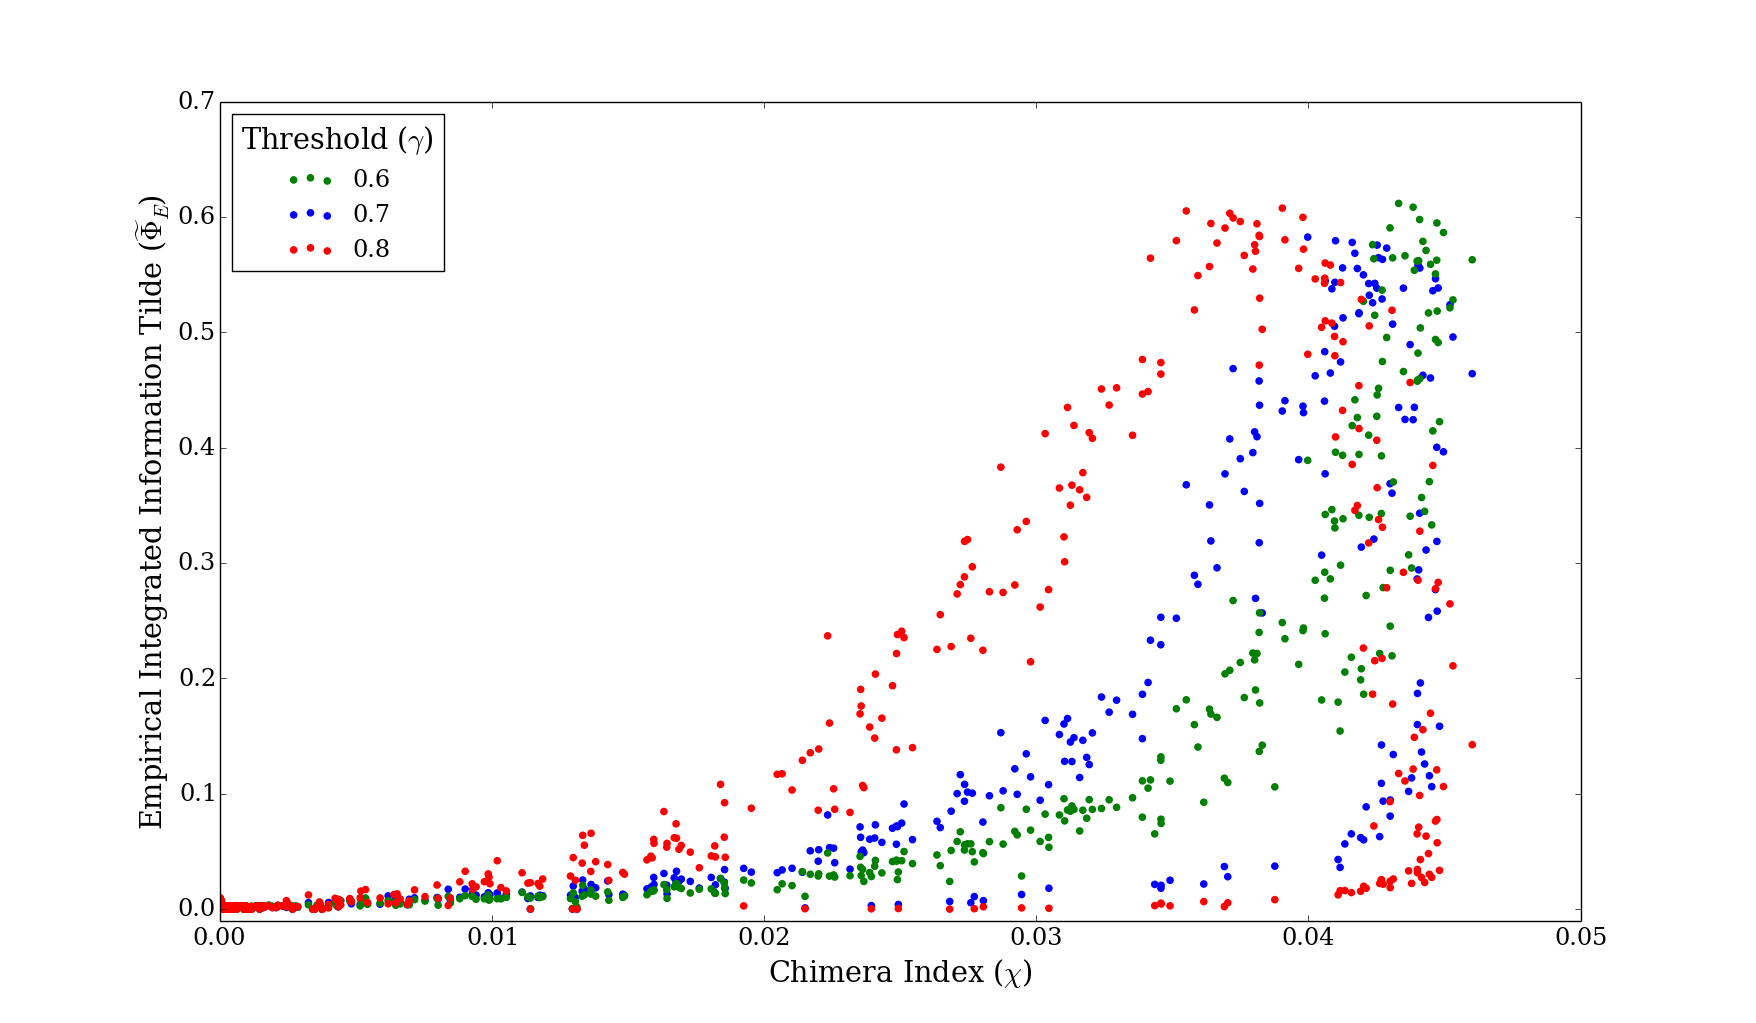
\includegraphics[scale = 0.35]{figures/phi_tilde_vs_chi_mid}
\caption{
	Empirical Integrated Information Tilde ($\widetilde{\Phi}_E$) vs Chimera Index ($\chi$) at mid-range synchronisation thresholds ($\gamma$).
	\label{fig:phi-tilde-vs-chi-mid}
}
\end{center}
\end{figure}

% ------------------------
% Phi vs Coalition Entropy
% ------------------------
\subsubsection{Empirical Integrated Information ($\Phi_{E}$) vs Coalition Entropy ($H_C$)}
\label{sec:app:osc:res:phi-v-hc}

We continued our analysis by exploring the relationship between integrated information and coalition entropy ($H_C$). As defined in Section \ref{sec:bg:hc}, coalition entropy measures the occurrence of the various states entered by a system given the space of all possible states it can enter. Nevertheless, coalition entropy does not take into account any past state given a current state, and so it is agnostic to the order in which the states actually occur. This is implied in its definition in Equation \ref{eq:hc}. As integrated information does take into consideration the order in which states occur, it is of particular interest to analyse its relationship with $H_C$.

We first plotted $\Phi_E$ against $H_C$, as shown in Figure \ref{fig:phi-vs-hc-multi}. We can see that for all thresholds, the plots from an exponential-like pattern. Obviating $\gamma = 0.9$, we observe that there is a heavy overlap between the various thresholds, with all of them reaching a maximum of $\Phi_E \approx 0.5$ as $H_C$ approaches one.

\begin{figure}[H]
\begin{center}
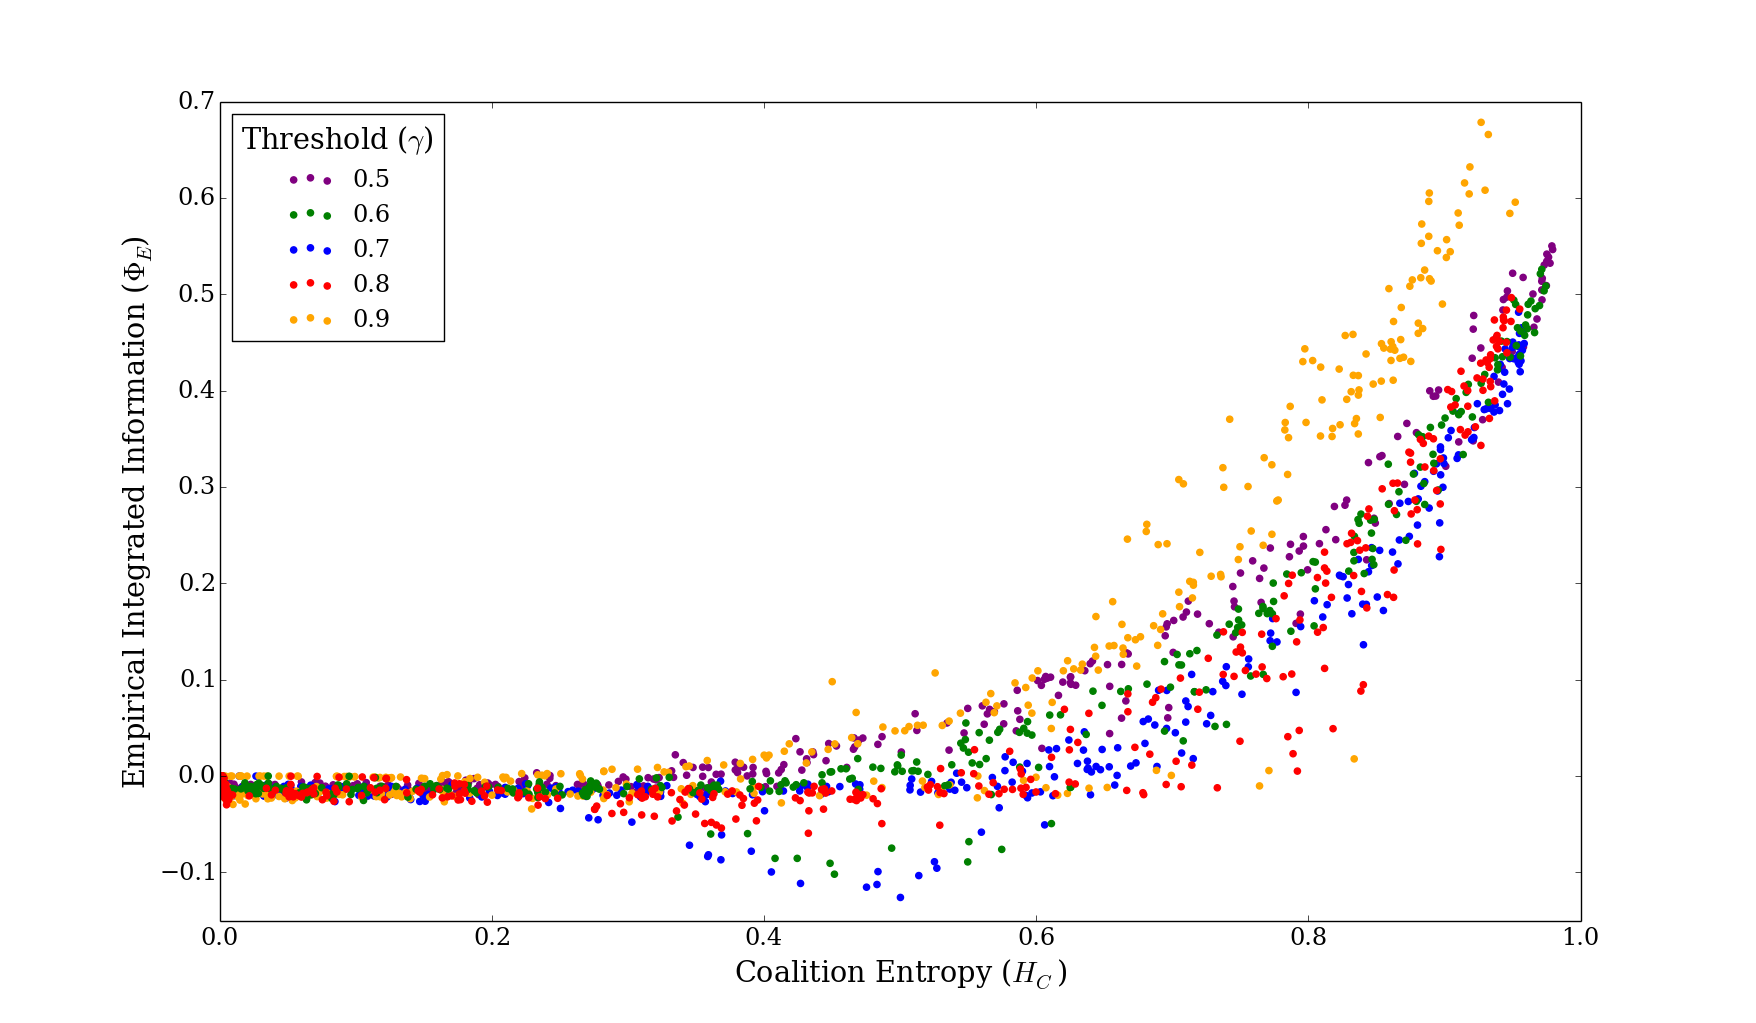
\includegraphics[scale = 0.35]{figures/phi_vs_hc_multi}
\caption{
		Empirical Integrated Information ($\Phi_E$) vs Coalition Entropy ($H_C$).
	\label{fig:phi-vs-hc-multi}
}
\end{center}
\end{figure}

% ------------------------------
% Phi Tilde vs Coalition Entropy
% ------------------------------
\subsubsection{Empirical Integrated Information Tilde ($\widetilde{\Phi}_{E}$) vs Coalition Entropy ($H_C$)}
\label{sec:app:osc:res:phi-tilde-v-hc}

We then examined $\widetilde{\Phi}_{E}$ against $H_C$, as shown in Figure \ref{fig:phi-tilde-vs-hc-multi}. The result is similar to the one for $\Phi_E$ in Section \ref{sec:app:osc:res:phi-v-hc}, with data from all thresholds forming an exponential-like pattern. Once more, if we ignore $\gamma = 0.9$, there is a consistent overlap between all other values of $\gamma$. Additionally, aside from $\gamma = 0.9$, there is considerably less noise, with only a few outliers at $H_C \approx 0.6$.

\begin{figure}[H]
\begin{center}
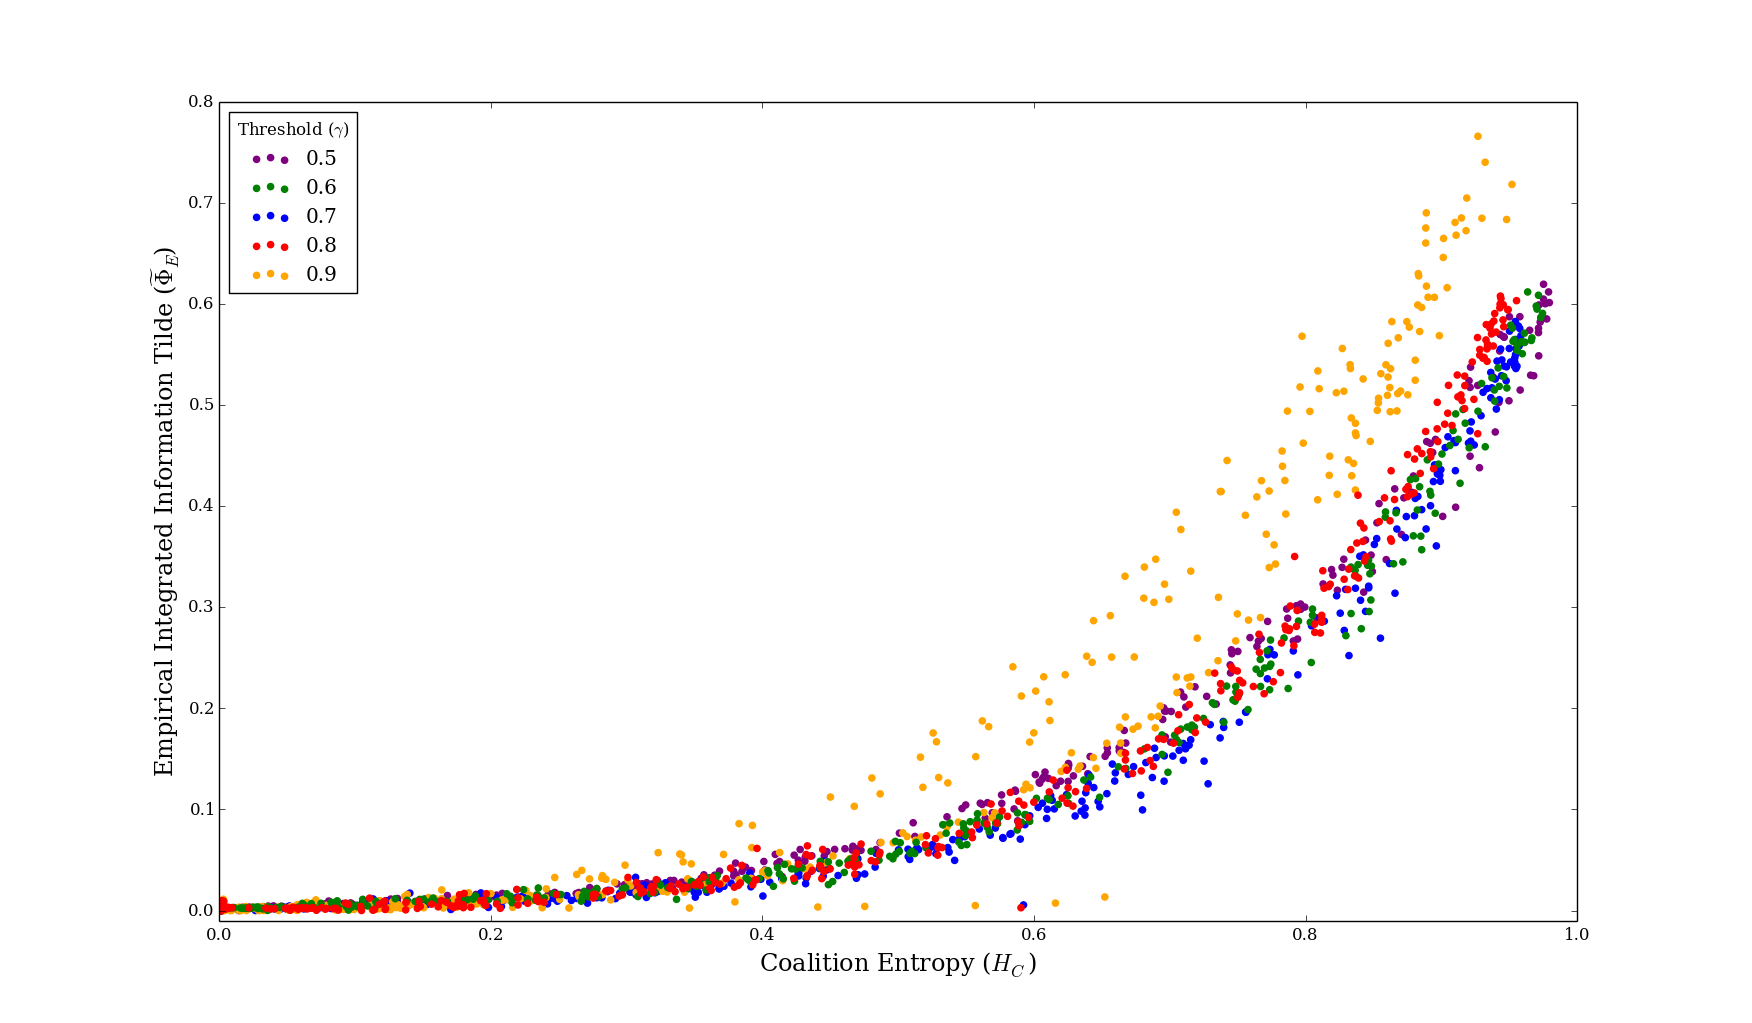
\includegraphics[scale = 0.35]{figures/phi_tilde_vs_hc_multi}
\caption{
	Empirical Integrated Information Tilde ($\widetilde{\Phi}_E$) vs Coalition Entropy ($H_C$).
	\label{fig:phi-tilde-vs-hc-multi}
}
\end{center}
\end{figure}


% ----------------
% Phi Tilde vs Phi
% ----------------
\subsubsection{Empirical Integrated Information Tilde ($\widetilde{\Phi}_{E}$) vs Empirical Integrated Information ($\Phi_{E}$)}

We were also interested in investigating the relationship between $\Phi_{E}$ and $\widetilde{\Phi}_{E}$. Thus, for each simulation, we plotted the value we obtained for $\widetilde{\Phi}_{E}$ against the one for $\Phi_E$, as shown in Figure \ref{fig:phi-tilde-vs-phi}. We observed a general positive correlation, with $\widetilde{\Phi}_{E}$ being higher than its respective $\Phi_E$ value, as can be observed by the fact that the plotted points are consistently above the $\widetilde{\Phi}_{E} = \Phi_E$ line in the dashed black line. Additionally, we can see that for values of $\Phi_E \approx 0$, there was more inconsistency with regards to the corresponding value $\widetilde{\Phi}_{E}$.

\begin{figure}[H]
\begin{center}
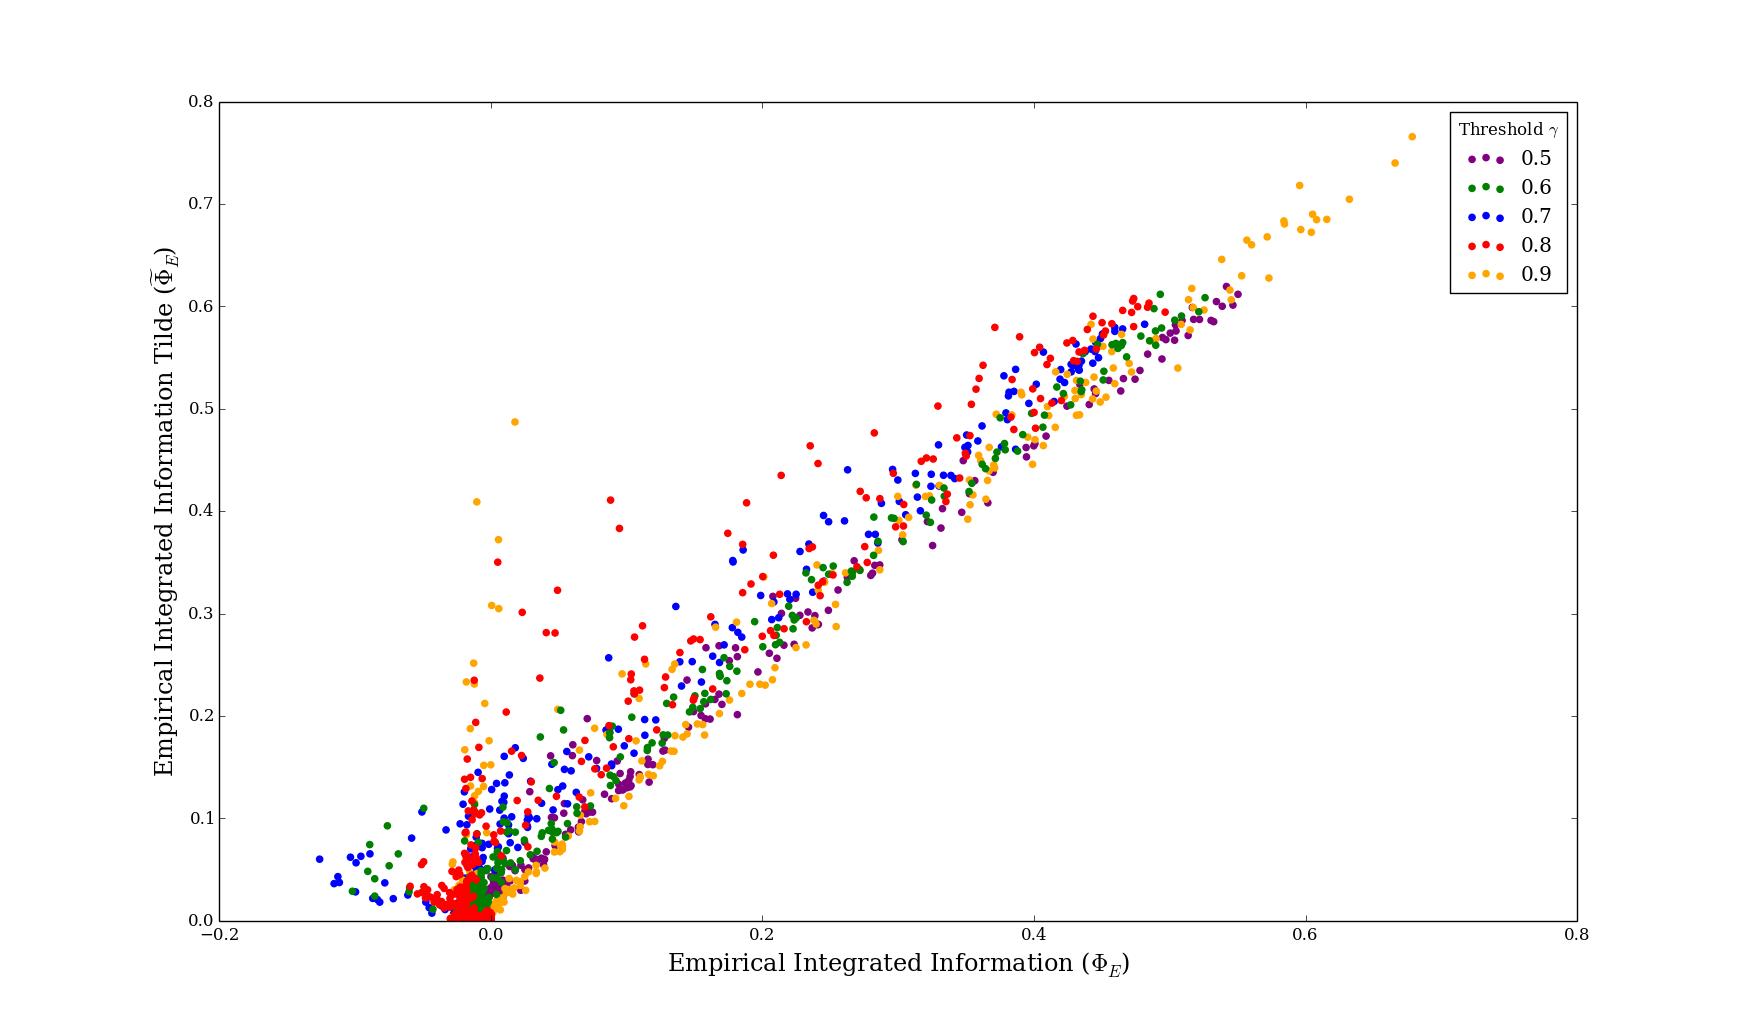
\includegraphics[scale = 0.35]{figures/phi_tilde_vs_phi}
\caption{
	Empirical Integrated Information Tilde ($\widetilde{\Phi}_E$) vs Empirical Integrated Information ($\Phi_E$).
	\label{fig:phi-tilde-vs-phi}
}
\end{center}
\end{figure}

\subsection{Surrogate Data Analysis}
\label{sec:app:osc:surrogate}

In order to provide insight into the robustness of our results concerning integrated information, we conducted some analysis using surrogate data. For our purposes we used both transformations of data generated by the oscillator simulations as well as synthetic data generated based on predefined models. We examined not only how our surrogate data analysis affected $\Phi_E$ and $\widetilde{\Phi}_E$, but also mutual information, as this measure is  the key building block of $\Phi_E$.

\subsubsection{Sorted Time Series}

In order to sort the time series by state, we took advantage of the \texttt{reduce} function in our \texttt{Input} class. As described in Section \ref{sec:impl:ei}, \texttt{reduce} takes the two-dimensional time series matrix and assigns a unique state integer for each possible vector value. The output is a one-dimensional array of states, which we could then sort using Java's inbuilt `Arrays.sort` method. We then computed coalition entropy, empirical integrated information and empirical integrated information tilde for each of the 7500 simulations and stored the results for comparison with the original values.

As expected, coalition entropy was not affected by the sorting operation, given that it is agnostic to the order in which each coalition appears, as discussed in Section \ref{sec:app:osc:res:phi-v-hc}. This is shown in Figure \ref{fig:hc_sorted_vs_hc}.

\begin{figure}[H]
\begin{center}
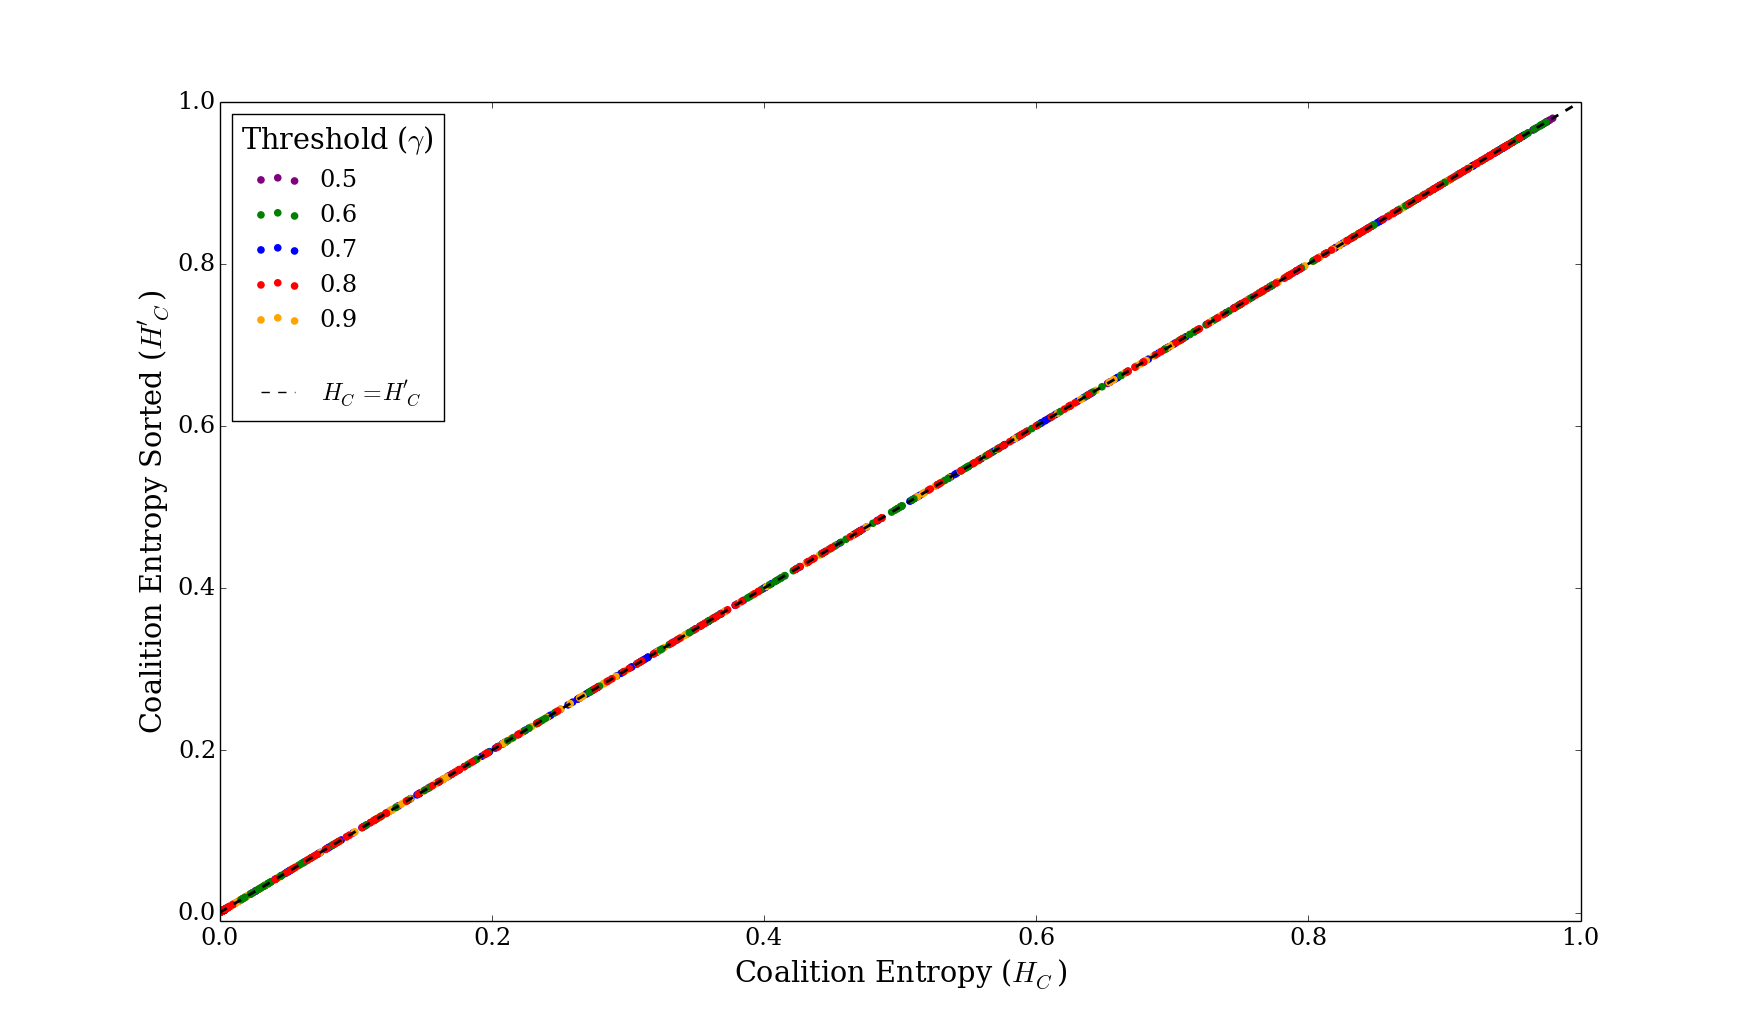
\includegraphics[scale = 0.35]{figures/hc_sorted_vs_hc}
\caption{
	Coalition Entropy Sorted ($H'_C$) vs Coalition Entropy ($H_C$).
	\label{fig:hc_sorted_vs_hc}
}
\end{center}
\end{figure}

However, given the nature of empirical integrated information, we expected that $\Phi_E$... . Figure \ref{fig:phi_sorted_vs_phi} shows how as the original value for $\Phi_E$ increases, the value for the sorted run, $\Phi'_E$ decreases. In fact, the vast majority of value for $\Phi'_E$ are negative. A similar phenomenon can be seen for $\widetilde{\Phi}$ as shown in Figure \ref{fig:phi_sorted_vs_phi}. 

\begin{figure}[H] 
	\label{fig:phi-vs-phi-sorted} 
	\begin{minipage}[b]{0.5\linewidth}
		\begin{figure}[H]
		\begin{center}
		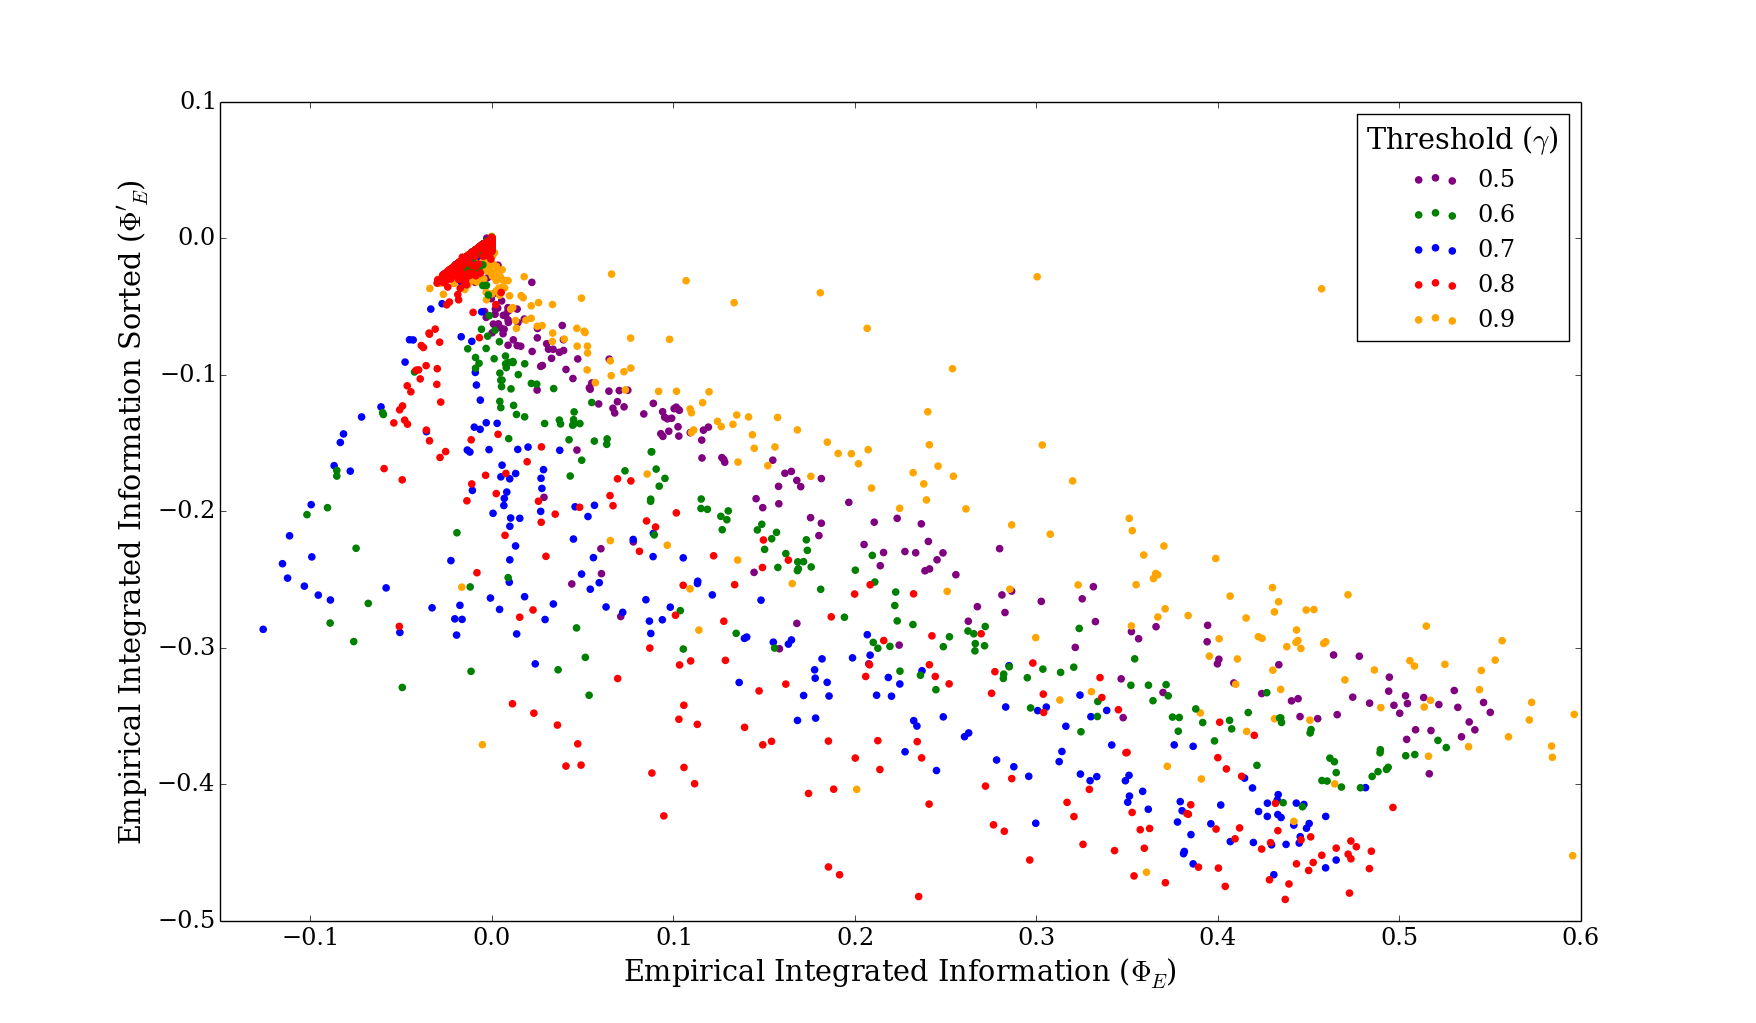
\includegraphics[scale = 0.2]{figures/phi_sorted_vs_phi}
		\caption{
			$\Phi'_E$ vs $\Phi_E$.
			\label{fig:phi_sorted_vs_phi}
		}
		\end{center}
		\end{figure}
		\vspace{2ex}
	\end{minipage}
	\begin{minipage}[b]{0.5\linewidth}
		\begin{figure}[H]
		\begin{center}
		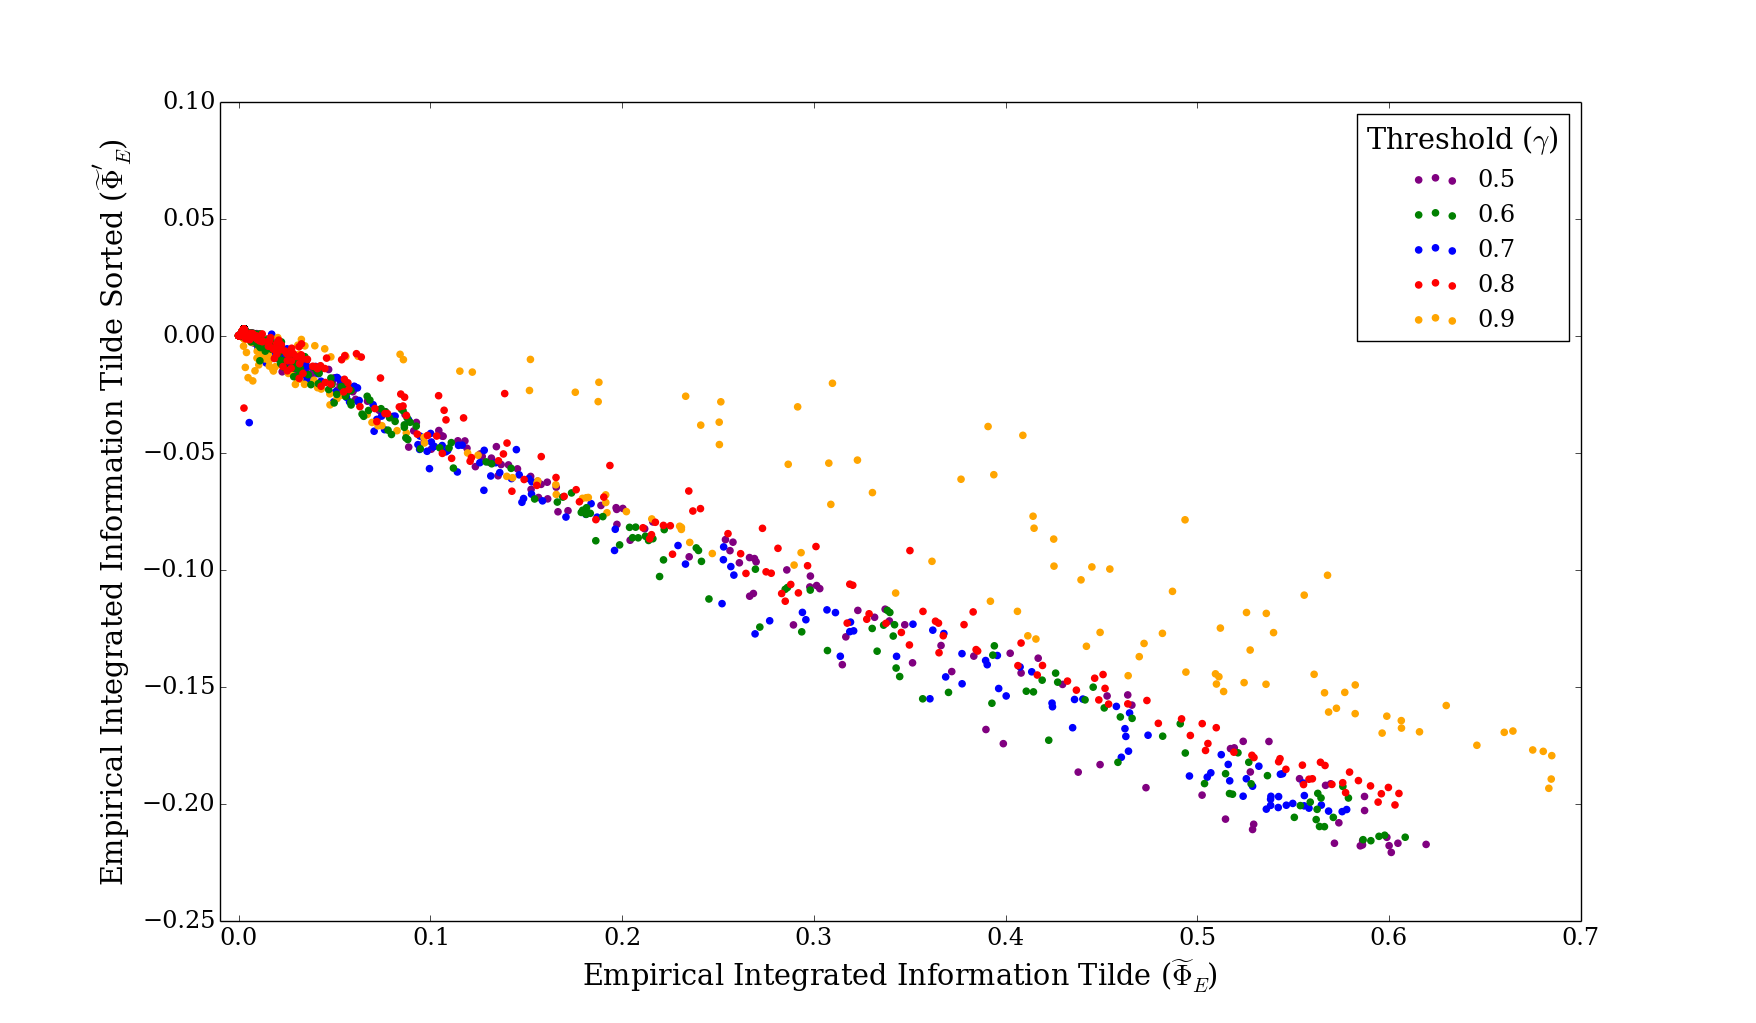
\includegraphics[scale = 0.2]{figures/phi_tilde_sorted_vs_phi_tilde}
		\caption{
			$\widetilde{\Phi}'_E$ vs $\widetilde{\Phi}_E$.
			\label{fig:phi_tilde_sorted_vs_phi_tilde}
		}
		\end{center}
		\end{figure}
		\vspace{2ex}
	\end{minipage}
\end{figure}


We can also see in Figure \ref{fig:phi_sorted_vs_hc}, how $\Phi'_E$, decreases as coalition entropy increases. For $\widetilde{\Phi}'_E$, this relationship is even more demarcated and consistent across all thresholds, as shown in Figure \ref{fig:phi_tilde_sorted_vs_hc}.

\begin{figure}[H] 
	\label{fig:phi-vs-hc-sorted} 
	\begin{minipage}[b]{0.5\linewidth}
		\begin{figure}[H]
		\begin{center}
		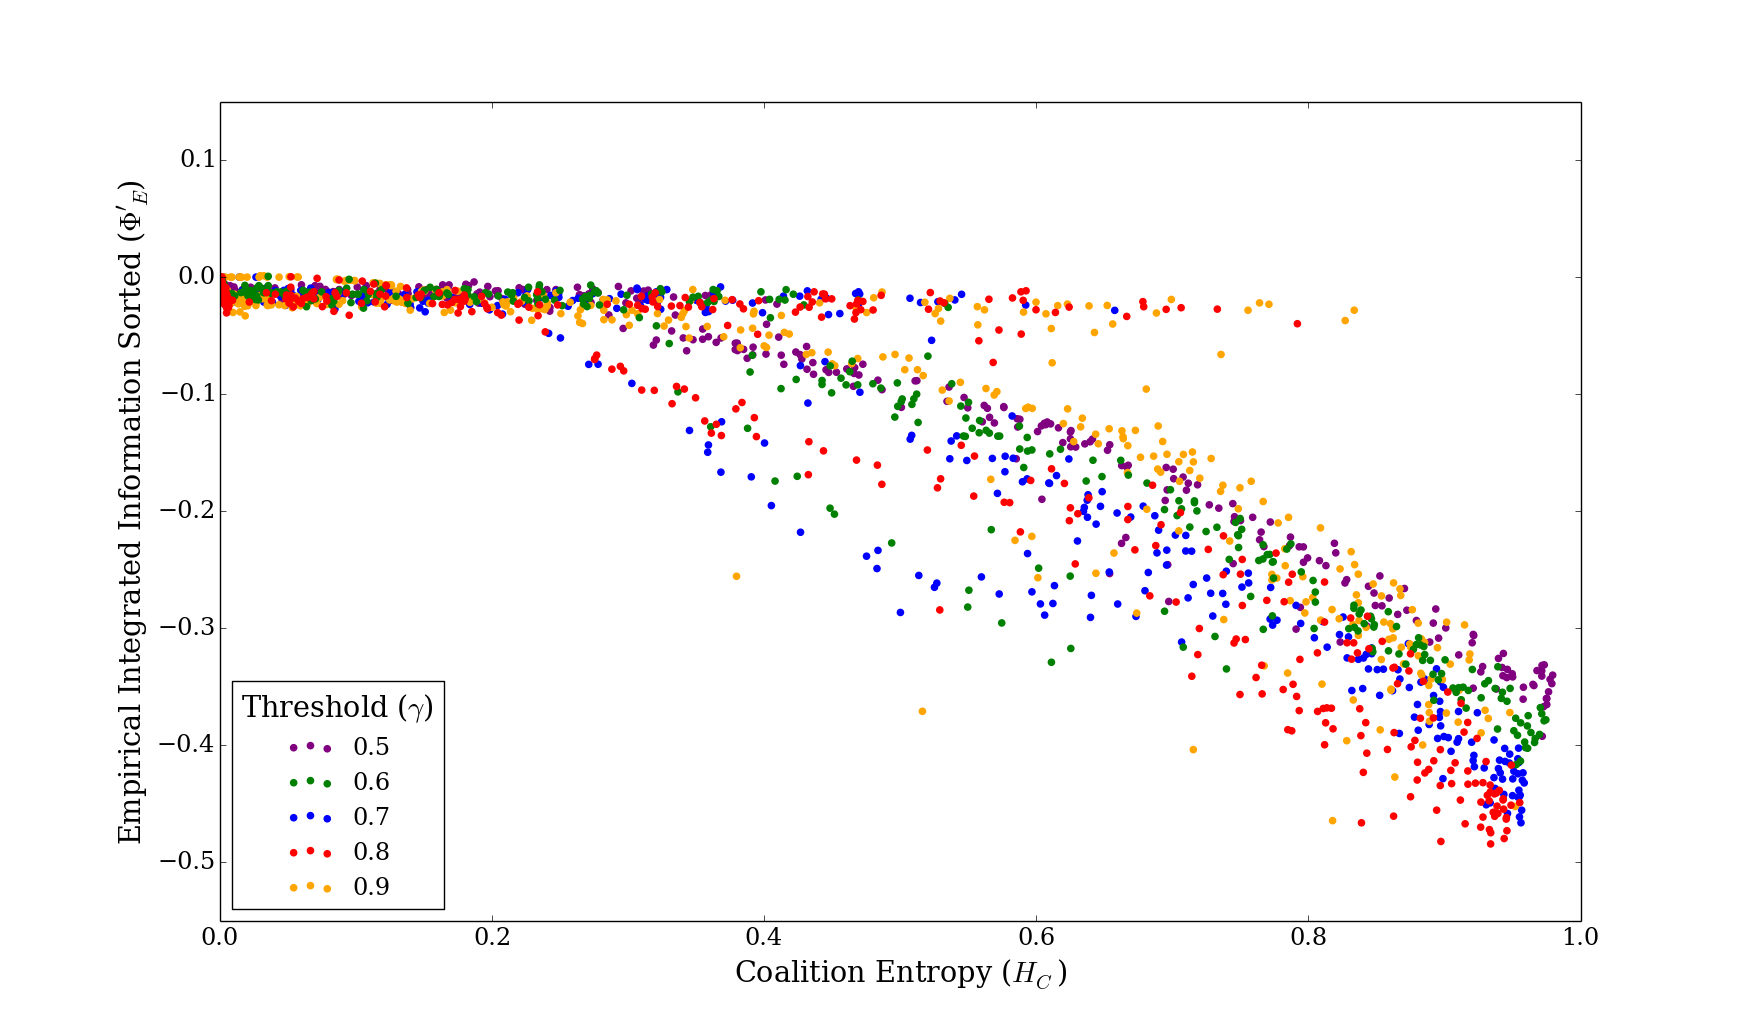
\includegraphics[scale = 0.2]{figures/phi_sorted_vs_hc}
		\caption{
			$\Phi'_E$ vs $H_C$.
			\label{fig:phi_sorted_vs_hc}
		}
		\end{center}
		\end{figure}
		\vspace{2ex}
	\end{minipage}
	\begin{minipage}[b]{0.5\linewidth}
		\begin{figure}[H]
		\begin{center}
		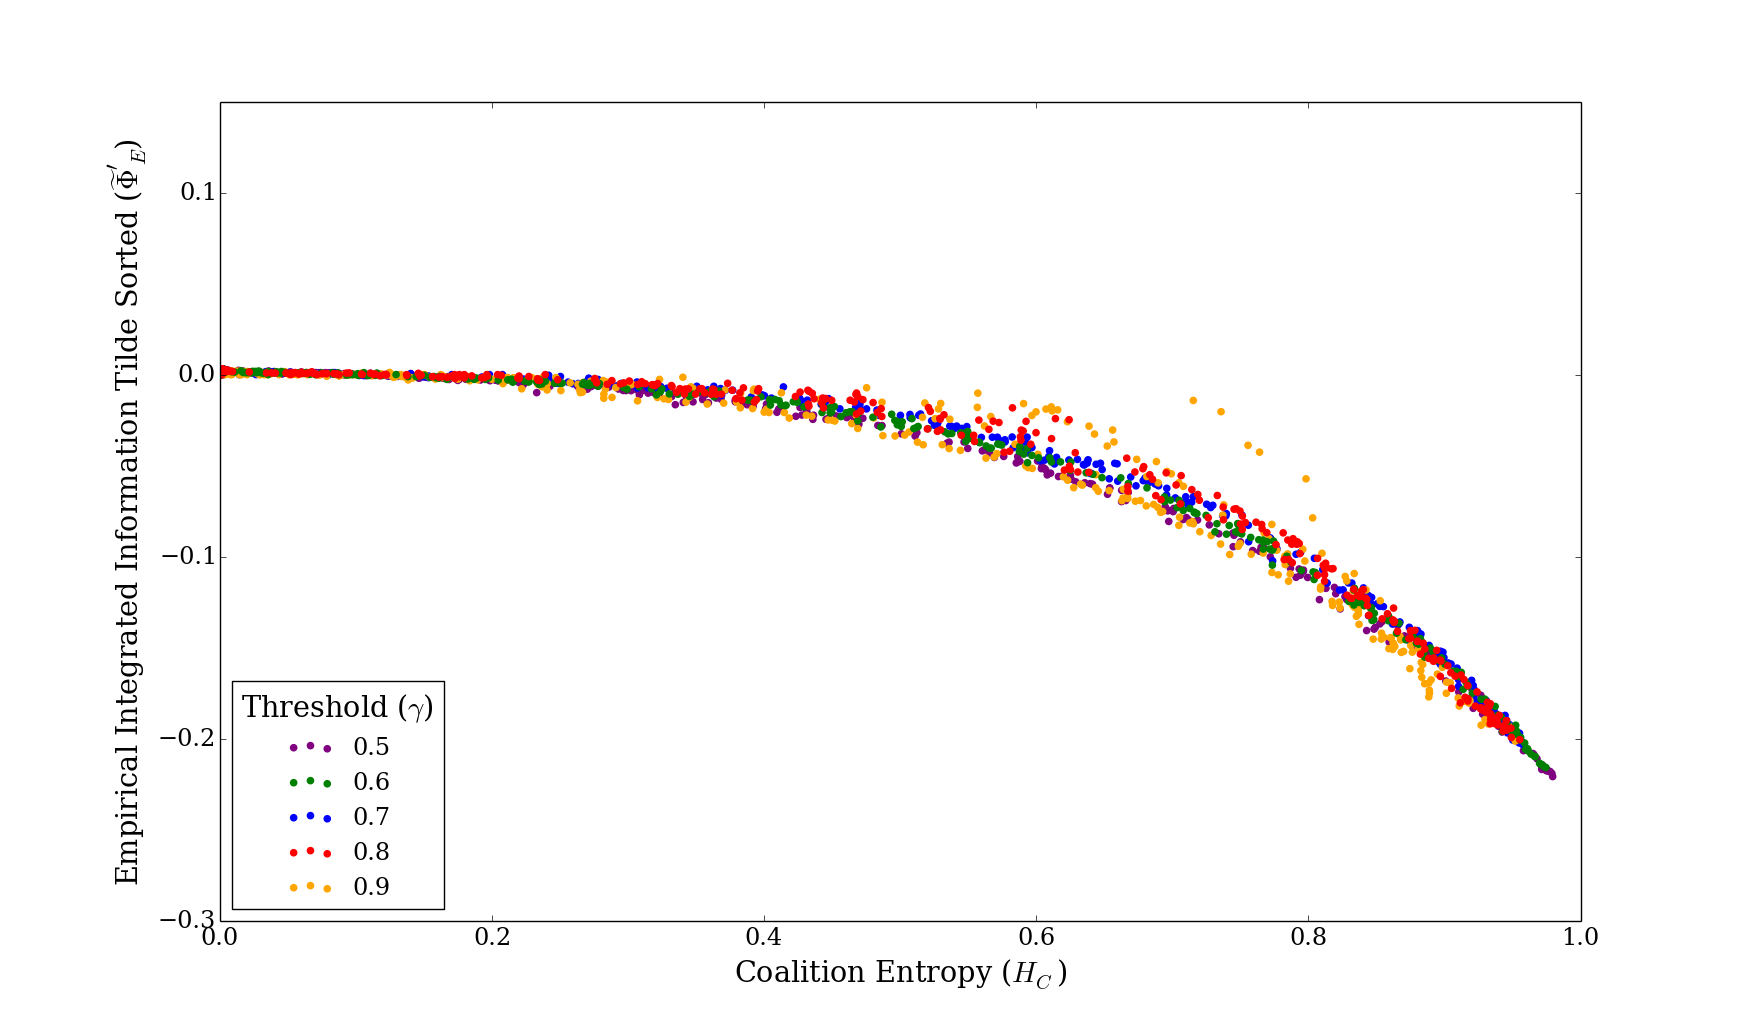
\includegraphics[scale = 0.2]{figures/phi_tilde_sorted_vs_hc}
		\caption{
			$\widetilde{\Phi}'_E$ vs $H_C$.
			\label{fig:phi_tilde_sorted_vs_hc}
		}
		\end{center}
		\end{figure}
		\vspace{2ex}
	\end{minipage}
\end{figure}


\subsubsection{Shuffled Time Series}

\subsubsection{Synthetic Data}

\subsection{Discussion}


\clearpage
\section{Application on Populations of Spiking Neurons}
\label{MSUSNN}

Based on the work by Buehlmann and Deco \cite{Buehlmann2010} as well as by Bhowmik and Shanahan \cite{Bhowmik2013}, we will model populations of neurons that exhibit synchrony, metastability and chimera states. By running simulations on these networks, we will create discrete time series output that can be fed into our implementation of $\Phi$. In contrast to the process explained in Section \ref{MSUKO}, by modelling synchronisation using actual spiking neurons, we gain access to more fine-grained properties of the network, such as its spectral complexity, given that various frequencies can be present in an oscillating population at any given point in time \cite{Bhowmik2013}. This allows us to record the correlation between these frequencies in each sample network, in addition to the measures recorded for the populations in systems of oscillators described in Section \ref{MSUKO}.

The first model will follow that used by Buehlmann and Deco and is depicted in Figure \ref{Buehlmann2010_Schema}. The simulations ran by Buehlmann and Deco consisted of 100 trials with each lasting six seconds, structured in the following manner, which we will replicate.
\begin{enumerate}
\item{No stimulus (400ms).}
\item{Presentation of the stimulus (5500ms).}
\item{No stimulus (100ms)}.
\end{enumerate}

\begin{figure}[H]
\centering
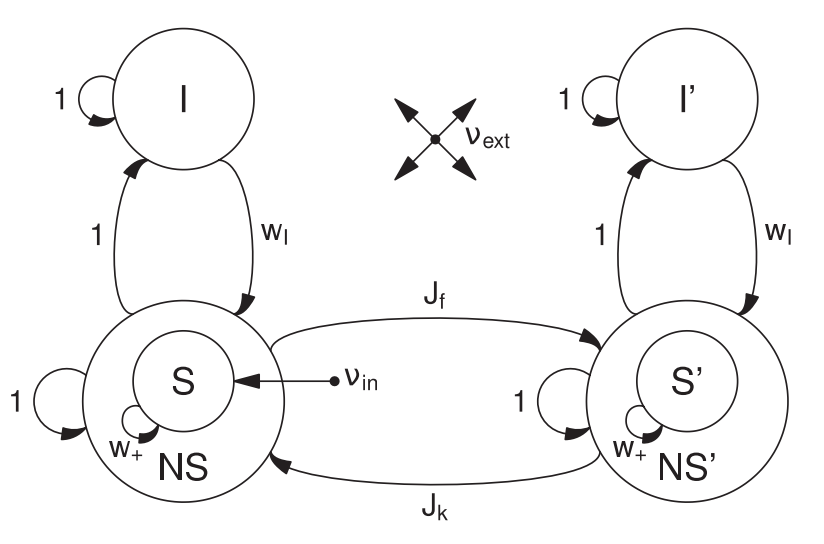
\includegraphics[scale = 0.75]{Buehlmann2010_Schema}
\caption{Schematic representation of the network used by Buehlmann and Deco. ``The network consists of two parts. In each part, there are excitatory (S, NS) and inhibitory (I) neurons.'' \cite{Buehlmann2010}}
\label{Buehlmann2010_Schema}
\end{figure}

The second model will follow that used by Bhowmik and Shanahan and is depicted in Figure \ref{Bhowmik2013_Schema}.

\begin{figure}[H]
\centering
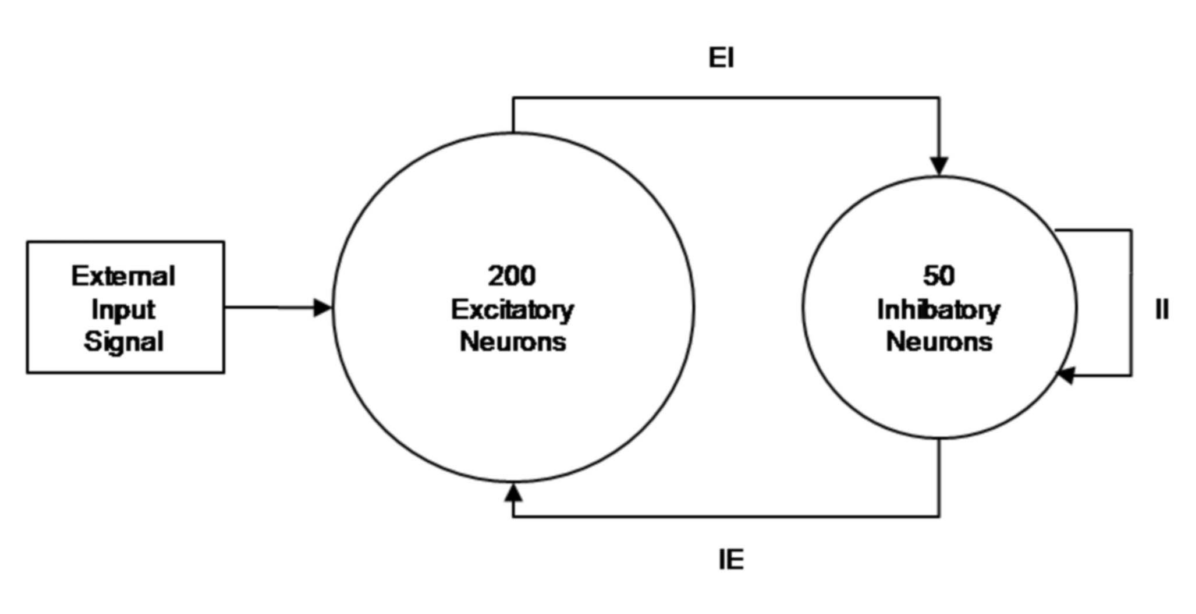
\includegraphics[scale = 0.75]{Bhowmik2013_Schema}
\caption{``The pyramidal inter-neuronal gamma (PING) architecture used for the neural oscillator nodes in the simulation experiments. To generate oscillator nodes of different frequencies for different neural models this base architecture was used with a genetic algorithm evolving the weights and delays for the synaptic connections.'' \cite{Bhowmik2013}}
\label{Bhowmik2013_Schema}
\end{figure}

\subsection{Methodology}
\subsection{Results}

\section{Future Work} \label{sec:fw}

\subsection{Ensure Robustness of $\Phi$ Implementation for JIDT}
\label{sec:fw:jidt}

One of the objectives of this project is to make the implementation of $\Phi$ for JIDT robust enough that it is included in the official distribution. In order to do this, once an initial working version of the implementation is finalised, we will send it to Lizier, who maintains the toolkit. By collaborating with Lizier, we aim to make conducting studies into integrated information using time series data more easily accessible for other researchers.

\subsubsection{Common Interface for $\Phi_E$ and $\widetilde{\Phi}_E$}

\subsubsection{Other Versions of $\Phi$}
Currently we have a working implementation of $\Phi_{E}$. In order to provide the user with flexibility, we aim to extend our contribution to JIDT to include other versions of $\Phi$ such as $\Phi_{DM}$ and $\Phi_{AR}$. This will allow the user to easily test the discrepancies between the different measures.

\subsubsection{Smoothing using Dirichlet Distribution}
The JIDT currently calculates mutual information for discrete data without taking into account the possibility that a state has not been observed given a relatively small input. This causes the probability of those unobserved states to be zero, potentially giving a skewed picture of the probability distribution. In order to correct for this, we will overload the JIDT's mutual information calculator for discrete data so that it can take an extra parameter $\alpha$. With this term we can then smooth the posterior distribution of the input data using a symmetric Dirichlet distribution with $\alpha$ as a prior.

\subsubsection{Testing}
In order to ensure that our implementation follows good software engineering practices and aligns itself with the tests provided by JIDT, we will write a variety of tests to cover both common and edge cases of our implementations of $\Phi$ and $\phi$ as well as our helper classes. We will do this using JUnit, as this is the testing framework used by default by JIDT.


% ==========
% References
% ==========
\clearpage
\bibliographystyle{plain}
\bibliography{report}{}
\clearpage

\end{document}